\chapter{Experimentos numéricos}
\section{Aplicação em imagens sintéticas}\label{cap_acf_sec4}

A metodologia (\textbf{MLE}) desenvolvida na seção anterior será aplicada em uma imagem sintética baseada no artigo \citep{gamf}, as quais são chamadas de \textit{Phantons}. As figuras desta seção serão geradas com auxílio dos códigos na linguagem Matlab, os programas foram disponibilizados pelos autores do artigo e estão localizados em  \url{http://www.ctim.es/polsar/}.

Inicialmente vamos gerar uma imagem sintética de dimensão $400\times400$ com duas amostras ou duas classes para validar as ideias do método (\textbf{MLE}), dessa maneira, vamos descrever como geramos a figura (\ref{cap_acf_fig01}). 

As imagens sintéticas em geral tem o intuito de auxiliar no estudo de diferentes métodos para tratamento de imagens. As imagens sintéticas construídas nesta seção  terão a tarefa de estudar como ocorre a transição entre duas amostras, ou seja, detectar evidências de bordas. 

A imagem PolSAR simulada usa a combinação de  matrizes de covariância $\{\Sigma_{k}\}_{k=1\dots 2}$ extraídas de uma imagem PolSAR real, com auxílio da distribuição complexa de Wishart $W_G(\Sigma, L)$, adicionalmente, na presente seção, os experimentos apresentados usam número de visadas $L=4$.

Para cada par de matrizes de covariância $\Sigma_{k_1}$, $\Sigma_{k_2}$ (com $k_2>k_1$) será gerado uma imagem PolSAR $P_{k_1,k_2,\beta}$ da seguinte maneira, em cada pixel branco da imagem sintética será agregado a amostra proveniente de $W_G(\Sigma_{k_1}, L)$ e de cada pixel preto da imagem sintética será agregado a amostra proveniente de $W_G(\Sigma_{k_2},L)$. Se necessário podemos fazer mistura de duas amostras tomando a combinação linear $W_G(\beta\Sigma_{k_1}+(1-\beta)\Sigma_{k_2}, L)$ com $\beta\in[0,1]$.

O parâmetro $\beta$ é usado para ponderar as informações entre as matrizes de covariância $\Sigma_{k_1}$ e $\Sigma_{k_2}$, modelando a mistura de classes em imagens PolSAR. Quando $\beta=0$ não há mistura e o problema consiste em escolher entre amostras puras de $\Sigma_{k_1}$ e $\Sigma_{k_2}$. Se o parâmetro $\beta$ se aproxima de $1$, teremos uma aproximação com a matriz de covariância $\Sigma_{k_1}$, assim teremos maior dificuldade de escolher classes. 

\begin{figure}[hbt]
\centering
	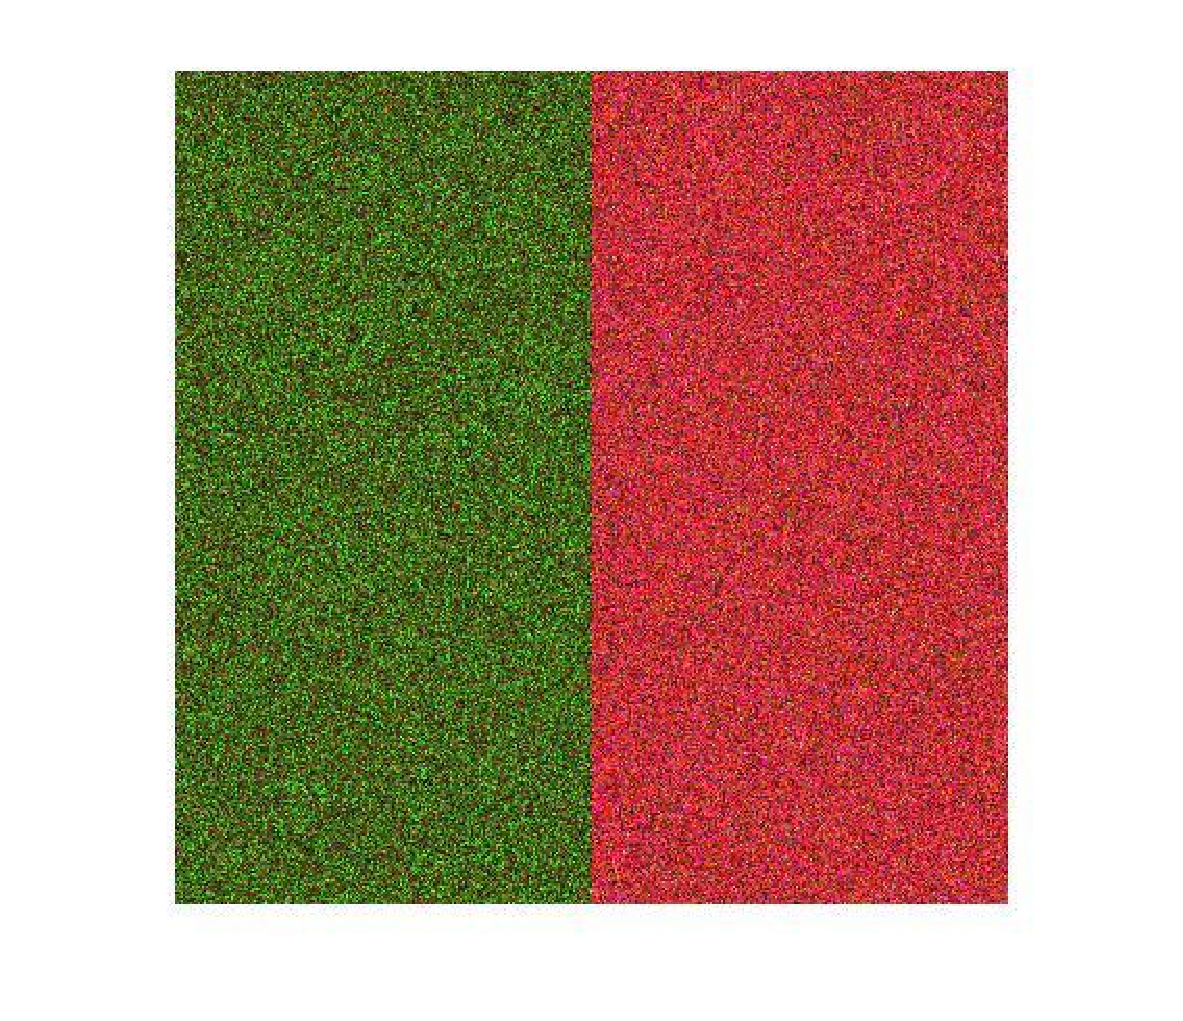
\includegraphics[width=5.0in]{phanton_nhfc_dec_pauli.pdf}
	\caption{Decomposição de Pauli para a phanton proposta no artigo de \citet{nhfc}.}\label{cap_acf_fig01}
\end{figure}
%%% ACF A decomposição de Pauli foi definida?
%%% AAB ver onde é melhor definir a decomposição de Pauli
A decomposição de Pauli foi usada na imagem mostrada na figura (\ref{cap_acf_fig01}), sendo que a mesma usa três canais da imagem \textbf{I} que são $\mathbf{I_{hh}}$, $\mathbf{I_{hv}}$ e $\mathbf{I_{vv}}$. 
	
\section{Aplicação do método \text{MLE} para duas classes definidas}

As informações sobre a imagem PolSAR podem ser obtidas de forma relativa pelos dados polarimétricos com respeito a um canal de dados, com intuito de resolver o problema de detecção bordas. Assumindo que o número de visadas $L$ e a matriz de covariância  $\Sigma$ são parâmetros na distribuição de Wishart, podemos descrever a distribuição gamma em cada canal, com densidade dada por 
\subsection{Distribuição gaussiana unidimensional para a intensidade}
\begin{equation}\label{cap_acf_23}
	f_{Z_{i}}(Z_{i};\mu,L)=\frac{L^{L}Z_{i}^{L-1}}{\mu^L\Gamma(L)} \exp(-L\frac{Z_i}{\mu}), \\
\end{equation}
sendo $i\in \{HH, VH, VV\}$, $\mu=\sigma_{i}^2$ a entrada $(i,i)$ da matriz $\Sigma$ e $Z_{i}$ a entrada $(i,i)$ da matriz randômica $\mathbf{Z}$. Podemos verificar essa expressão em \citep{fnc, nhfc, hsbmp}.	 

O primeiro teste numérico será realizado com $\Sigma_u$ e $\Sigma_f$ definidas por
\begin{equation}\label{matriz_sigma_nhfc_1}
	\hspace{2.75cm} \Sigma_{u}= \left[
\begin{array}{lll}
	962892             &19171 - 3579i&     -154638 + 191388i \\
	19171 + 3579i      &56707        &     -5798 + 16812i  \\
	-154638 - 191388i  &-5798 - 16812i&      472251 
\end{array}
\right],
\end{equation}
\begin{equation}\label{matriz_sigma_nhfc_2}
 \Sigma_{f}= \left[
\begin{array}{lll}
	360932            & 11050 + 3759i&   63896 + 1581i \\
	11050 - 3759i     & 98960       &   6593 + 6868i \\
	63896  - 1581i    & 6593  - 6868i&   208843
\end{array}
\right],
\end{equation}
onde os subescritos $u$ e $f$ definem respectivamente área urbana e floresta, extraídas de uma imagem real, podemos encontrar essas informações nos artigos \citep{fbgm, nhfc}.

De acordo com a função densidade de probabilidade (\ref{cap_acf_23}) e usando o canal $(hh)$ em ambas matrizes de covariância com $L=4$, podemos gerar a figura (\ref{cap_acf_fig02}), com a representação gráfica da função de densidade para os respectivos elementos $u$ e $f$ da matriz de covariância, neste caso, $\sigma_{hh}=962892$ e $\sigma_{hh}= 360932$. 

/\begin{figure}[hbt]
	\centering
	%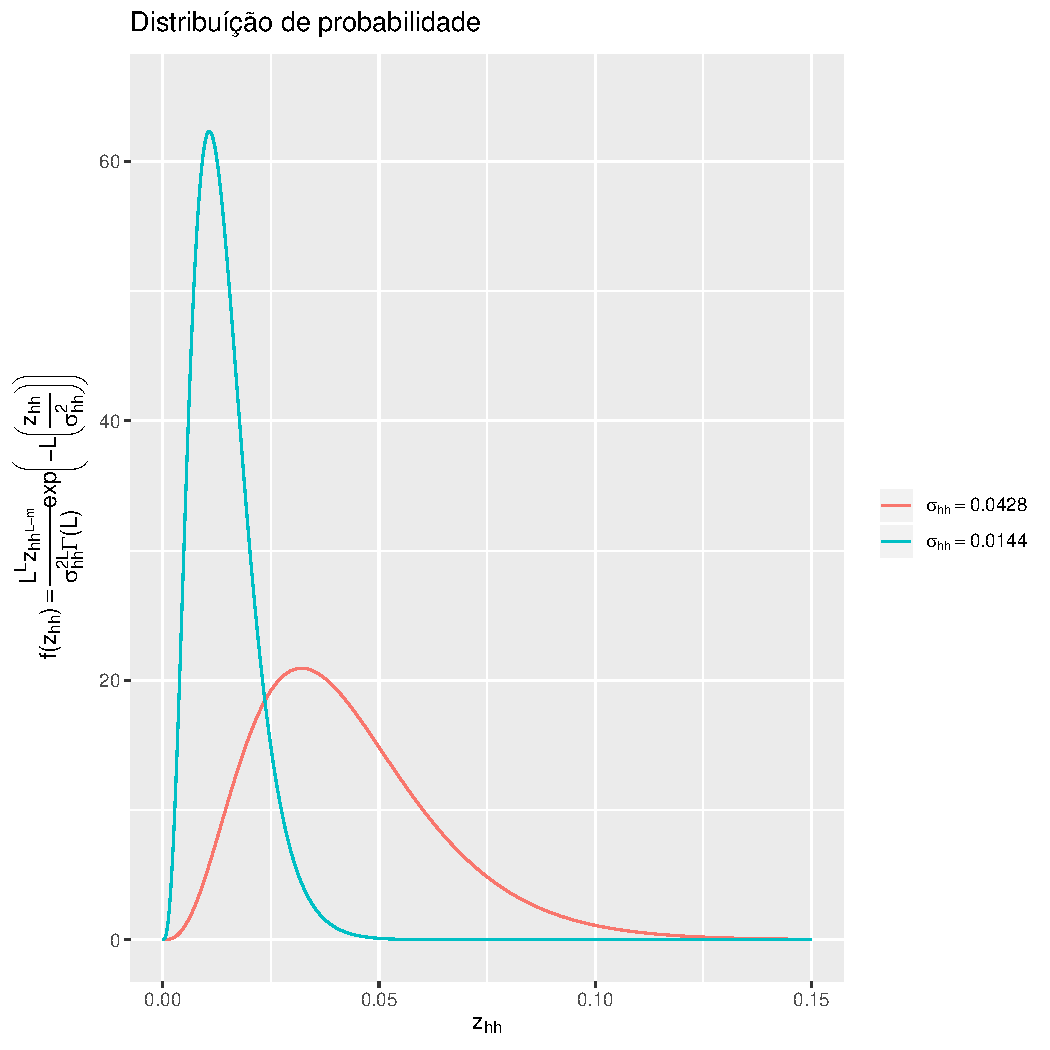
\includegraphics[scale = 1]{grafico_pdf_gamf_2017_sigma_hh.pdf}
  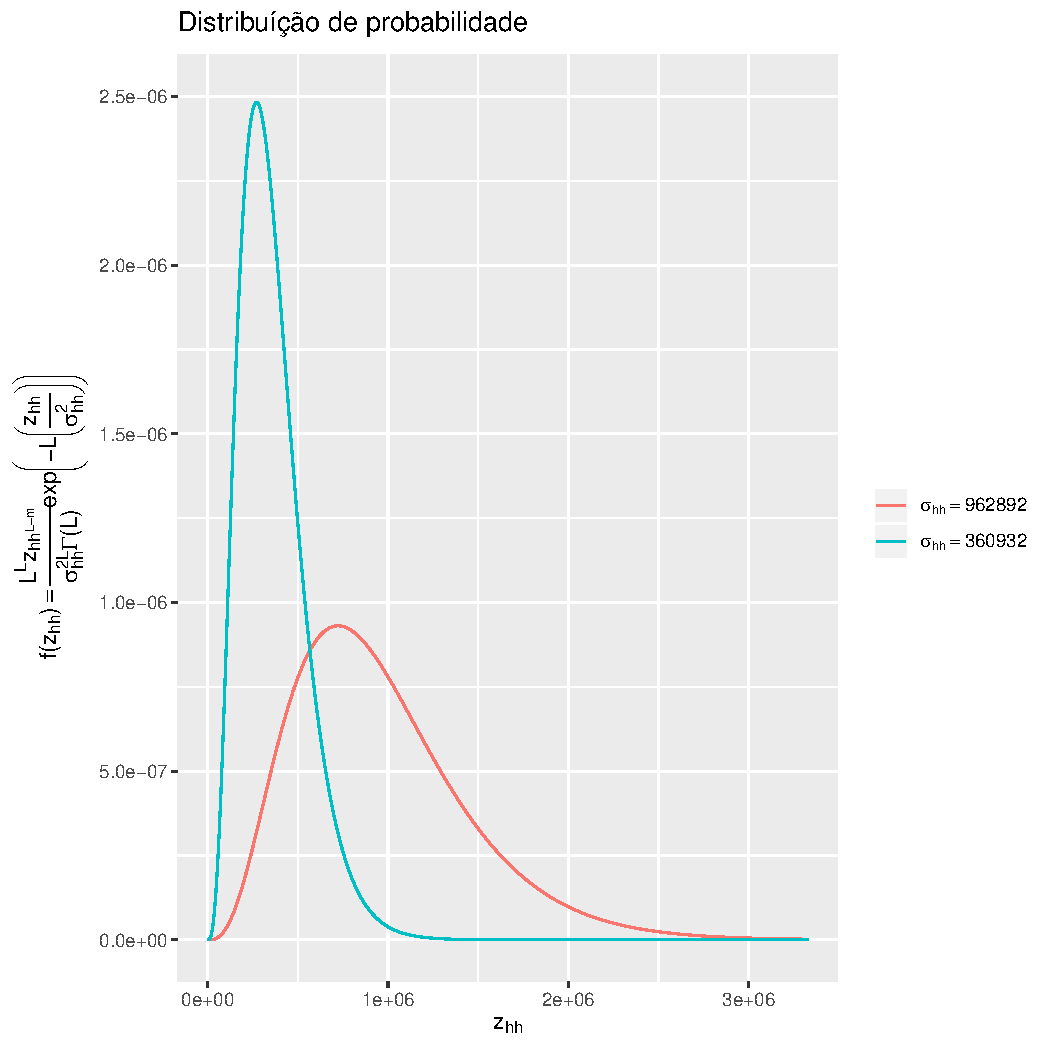
\includegraphics[scale = 0.7]{grafico_pdf_nhfc_2014_sigma_hh.pdf}
	\caption{Funções de densidade para dados simulados.}\label{cap_acf_fig02}
\end{figure}
%%% ACF Para fins de comparação, seria interessante ver as densidades no mesmo gráfico

A figura (\ref{cap_acf_fig01}) foi gerada com auxílio das distribuições Wishart descritas nas equações (\ref{cap_acf_13}) para $L=4$ e matrizes de covariância com $\Sigma_{u}$ e $\Sigma_{f}$ definidos em (\ref{cap_acf_24}) e (\ref{cap_acf_25}).

	
A imagem é construída com $400$ linhas distribuídas em duas bandas separadas verticalmente em torno do pixel $200$, lembrando que a imagem tem dimensão $400 \times 400$. Cada linha  tem duas amostras diferentes geradas com os parâmetros $\Sigma_{u}$ e $\Sigma_{f}$ respectivamente e ainda $L=4$ para as duas amostras.  

	O valor $200$ é fixado horizontalmente para termos uma linha contendo as duas amostras, para essa linha é calculado $l(j)$ conforme equação (\ref{cap_acf_21}) que deve ser aplicada nos canais $\mathbf{I_{hh}}$, $\mathbf{I_{vh}}$ e $\mathbf{I_{vv}}$.  
\begin{figure}[hbt]
\minipage{0.5\textwidth}
  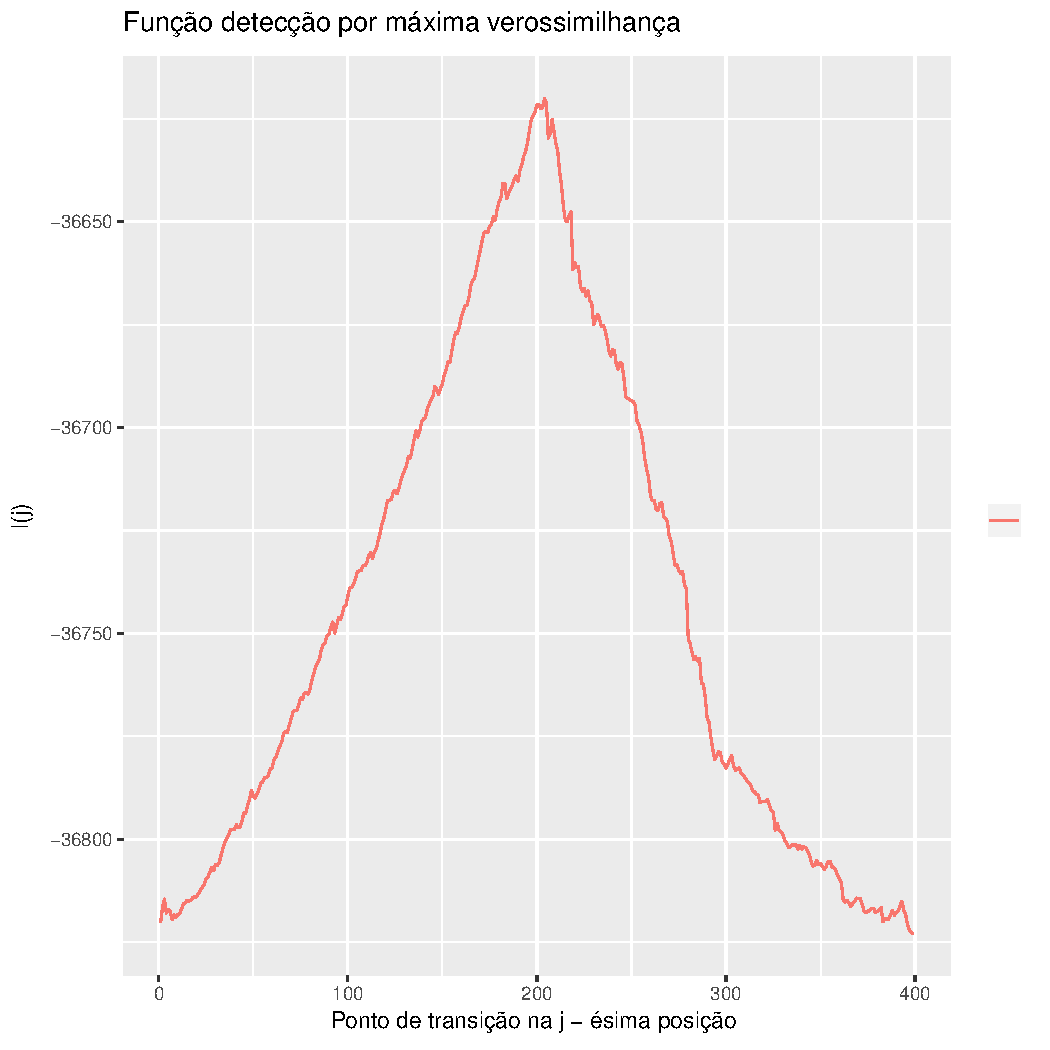
\includegraphics[width=\linewidth]{grafico_l_nhfc_2014_sigmahh.pdf}
	\caption{Função $l(j)$ para o canal $I_{HH}$}\label{cap_acf_fig04}
\endminipage\hfill
\minipage{0.5\textwidth}
  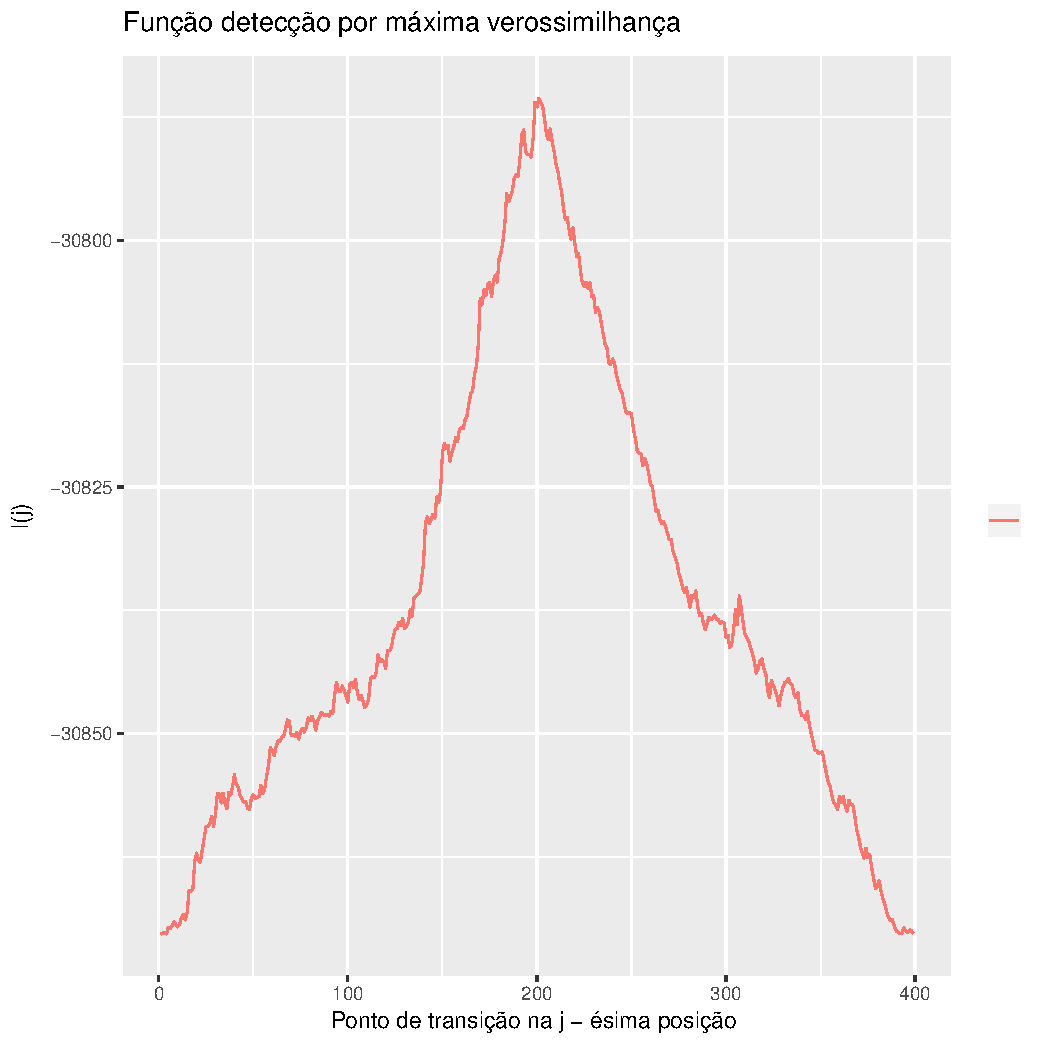
\includegraphics[width=\linewidth]{grafico_l_nhfc_2014_sigmahv.pdf}
	\caption{Função $l(j)$ para o canal $I_{HV}$}\label{cap_acf_fig05}
\endminipage\hfill
\centering
\minipage{0.5\textwidth}
  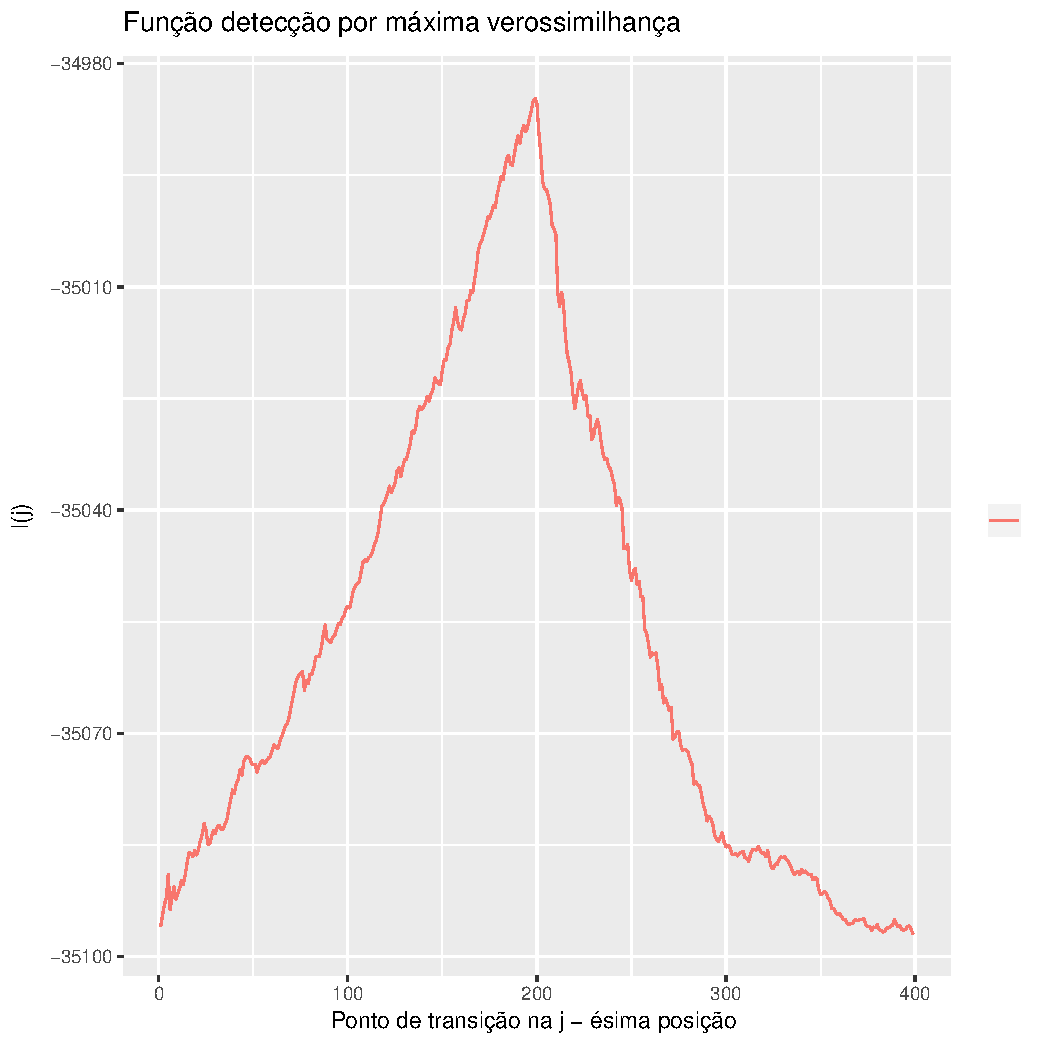
\includegraphics[width=\linewidth]{grafico_l_nhfc_2014_sigmavv.pdf}
	\caption{Função $l(j)$ para o canal $I_{VV}$}\label{cap_acf_fig06}
\endminipage\hfill
\end{figure}

	Podemos notar que as funções não são deriváveis em muitos pontos, então os métodos de otimização que necessitam do cálculo da derivada, terão funcionamento comprometido, resolvemos esse problema usando o método Simulated Anneling Generalizado (GenSA) que podemos encontrar na referência \citep{xgsh}.
	
	O método GenSA mostrou-se competitivo com os métodos empregados no artigo \citet{nhfc}, para testar a acurácia do GenSA e fazer a comparação com os métodos aplicados no artigo, vamos usar a métrica encontrada no artigo \citep{nhfc} e proposta na referência \citep{fbgm}.
        
	O erro foi calculado gerando $400$ replicações da distribuição Wishart com duas amostras como acima, gerando uma função $l(j)$ para cada replicação. Aplicando o GenSA para cada umas das $l(j)$ temos as evidências de bordas ou pontos de transição. O ponto de borda é $200$ por construção para todas as replicações, então o erro para cada replicação é o valor absoluto da diferença entre o ponto de borda e o valor estimado pelo método GenSA, portanto  
\begin{equation}\label{cap_acf_26}
\begin{array}{llll}
	E(r) &=& |200 - \hat{\jmath}(r)|, & 1\leq r \leq 400,  \\
\end{array}
\end{equation}
onde, $\hat{\jmath}(r)$ é o resultado da maximização de $l(j)$ pelo método GenSA na replicação $r$.

Usaremos frequências relativas para estimar a probabilidade de ter um erro menor que um número de pixeis. Denotando por $H(k)$ o número de replicações para qual o erro é menor que $k$ pixeis, então calculamos uma estimativa desta probabilidade por $f(k)=\frac{H(k)}{400}$. Nos testes realizados nesta seção variamos $k$ entre $1$ e $10$. O algoritmo está descrito em detalhes na referência \citep{fbgm}. 
\begin{figure}[hbt]
\minipage{0.475\textwidth}
\fbox{  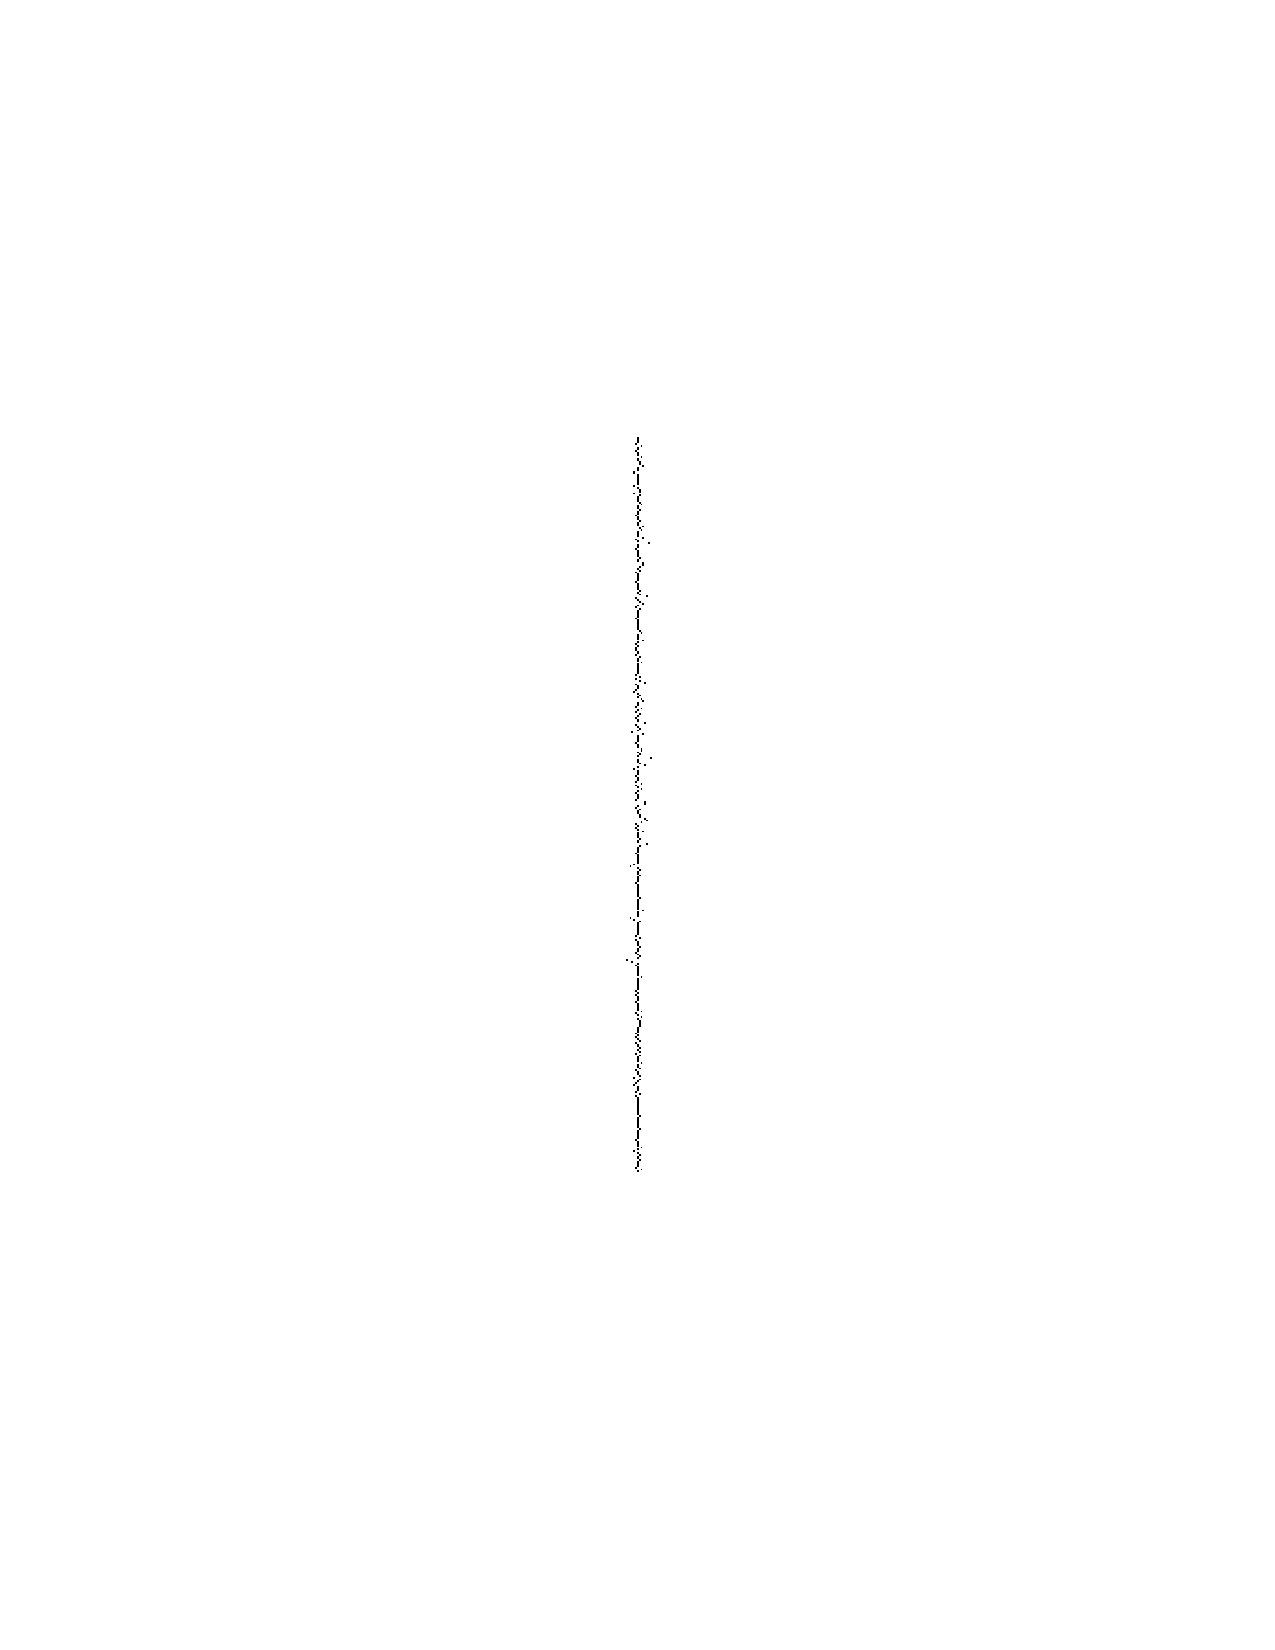
\includegraphics[width=\linewidth]{ev_hh_nhfc_2014.pdf}}
\caption{Evidências de bordas para o canal $I_{HH}$}\label{cap_acf_fig07}
\endminipage\hfill
\minipage{0.475\textwidth}
\fbox{ 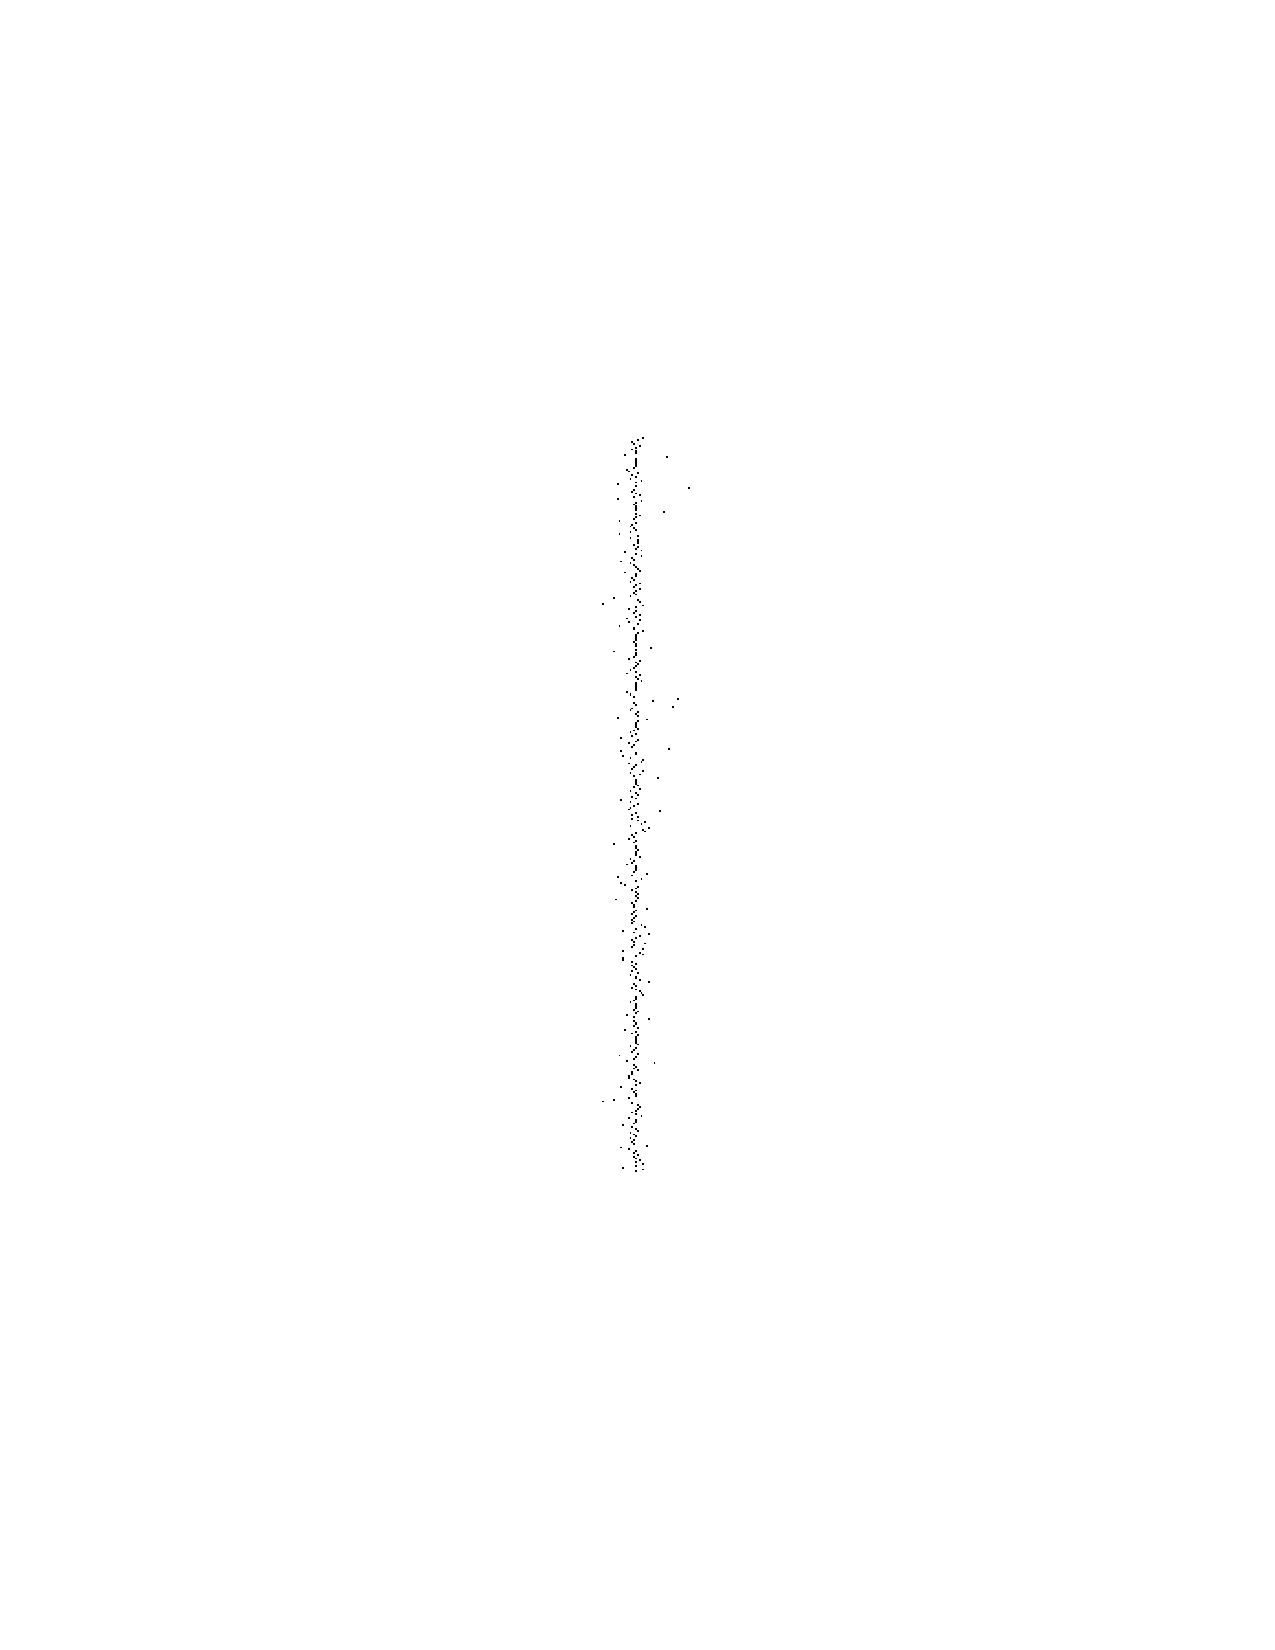
\includegraphics[width=\linewidth]{ev_hv_nhfc_2014.pdf}}
\caption{Evidências de bordas para o canal $I_{HV}$}\label{cap_acf_fig08}
\endminipage\hfill
\centering
\minipage{0.475\textwidth}
\fbox{ 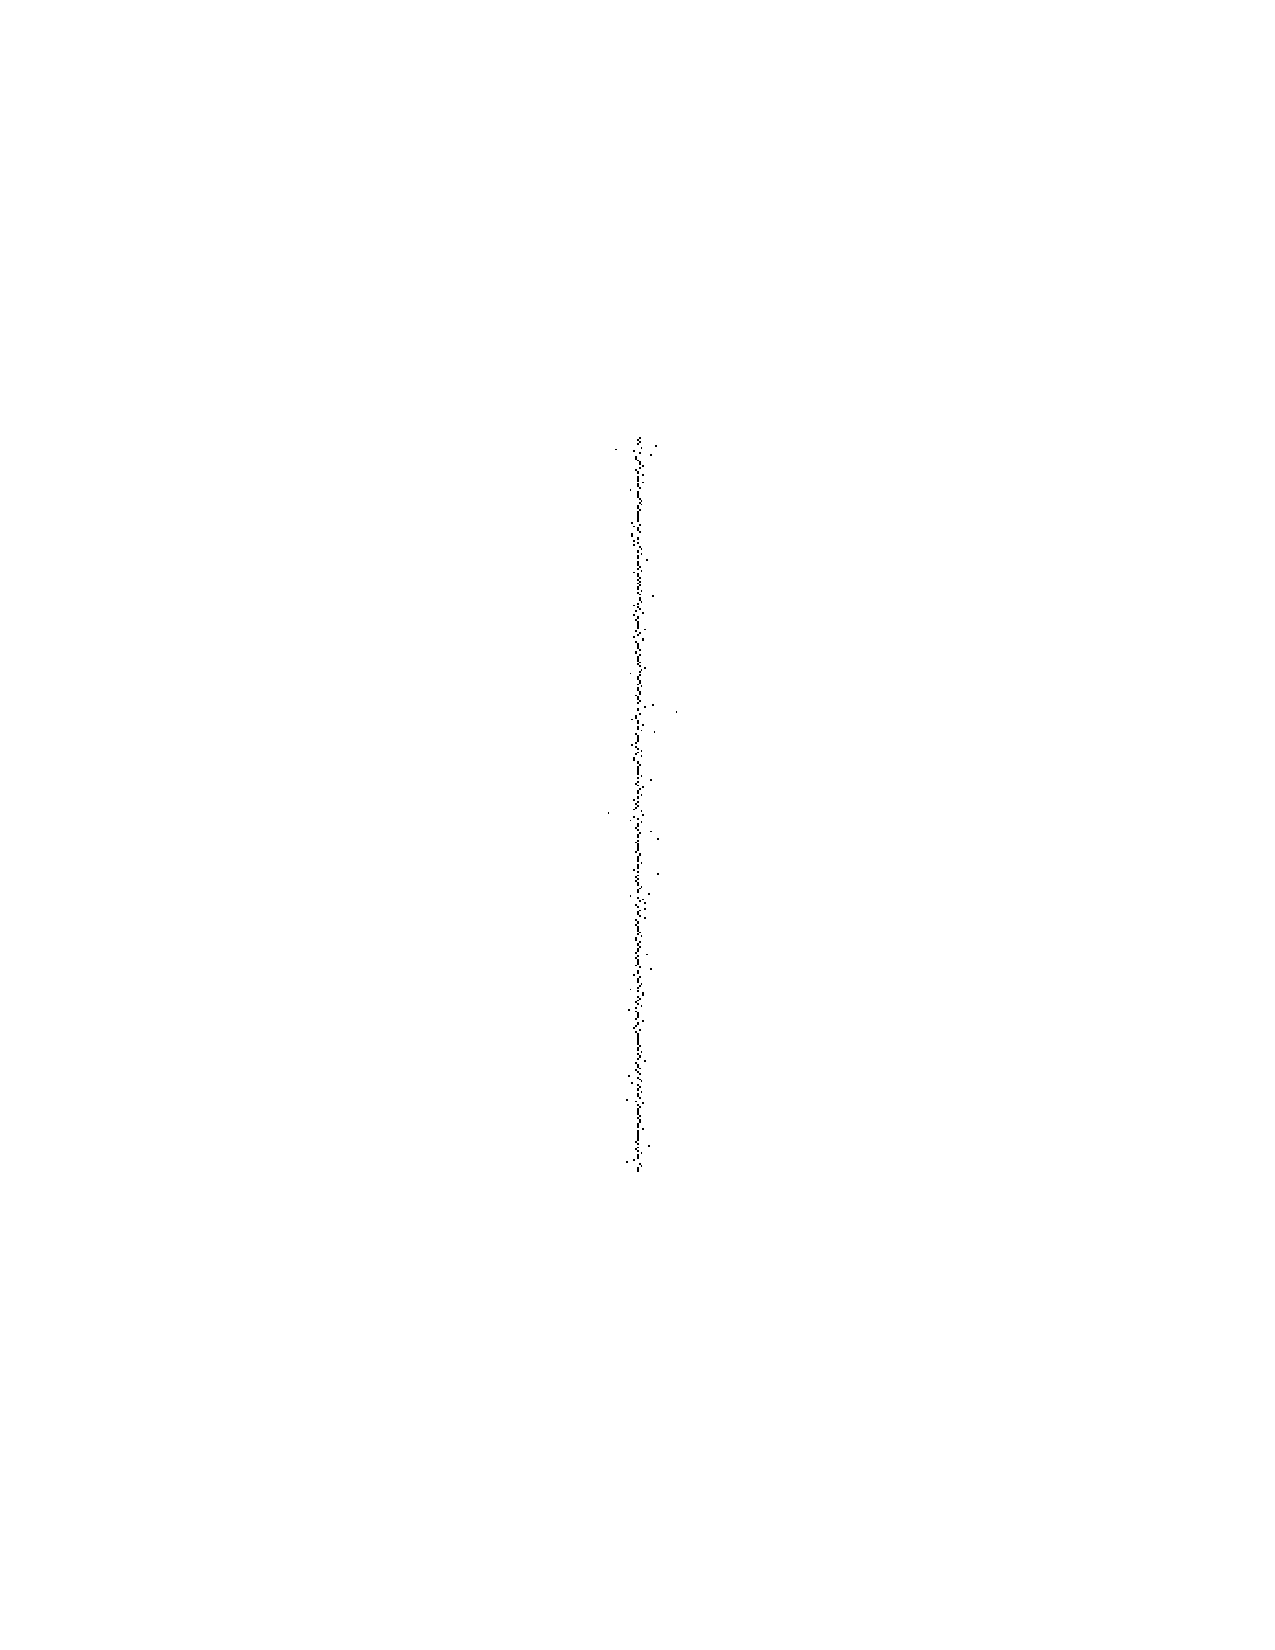
\includegraphics[width=\linewidth]{ev_vv_nhfc_2014.pdf}}
\caption{Evidências de bordas para o canal $I_{VV}$}\label{cap_acf_fig09}
\endminipage\hfill
\end{figure}

	A figura (\ref{cap_acf_fig10}) mostra as probabilidades para a detecção de bordas quando aplicado o método GenSA nos canais $I_{hh}$, $I_{vh}$ e $I_{vv}$ da imagem mostrada na figura (\ref{cap_acf_fig01}). As 400 replicações para cada canal e sua respectiva evidência de borda estão nas figuras (\ref{cap_acf_fig07}),(\ref{cap_acf_fig08}) e (\ref{cap_acf_fig09}).  
\begin{figure}[hbt]
\centering
	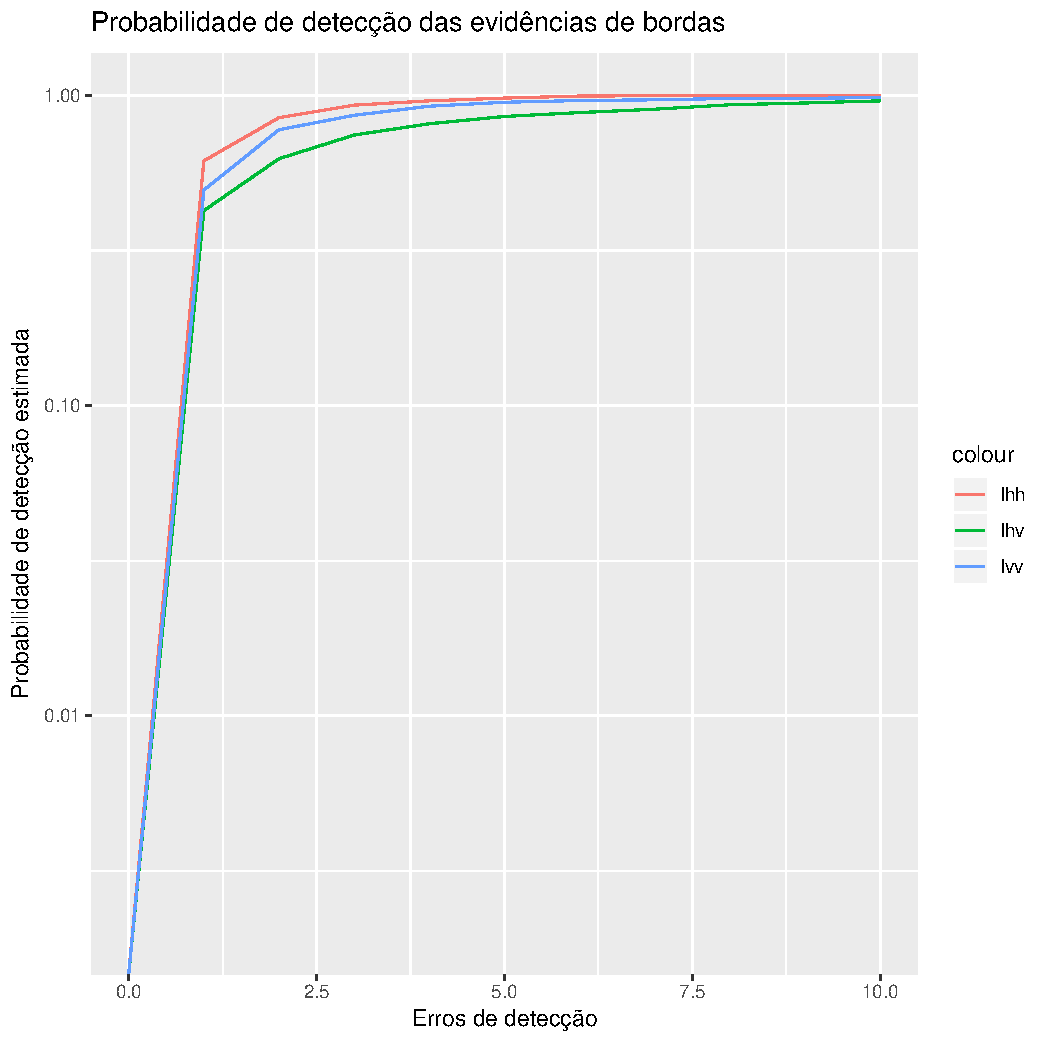
\includegraphics[width=5.0in]{metricas_ihh_ivh_ivv_nhfc.pdf}
	\caption{Probabilidade de detecção de borda estimada usando GenSA.}
\label{cap_acf_fig10}
\end{figure}


%\subsection{Distribuição multi visada para o interferograma}
%
%\begin{equation}
%\begin{array}{ccc}
%	f(\xi)&=&\frac{4L^{L+1}\xi^L}{\Gamma(L)(1-|\rho|^2)}I_0\left(\frac{2|\rho|L\xi}{1-|\rho|^2}\right)K_{L-1}\left(\frac{2L\xi}{1-|%\rho|^2}\right).
%		\end{array}
%\end{equation}

\begin{figure}[hbt]
	\centering
	%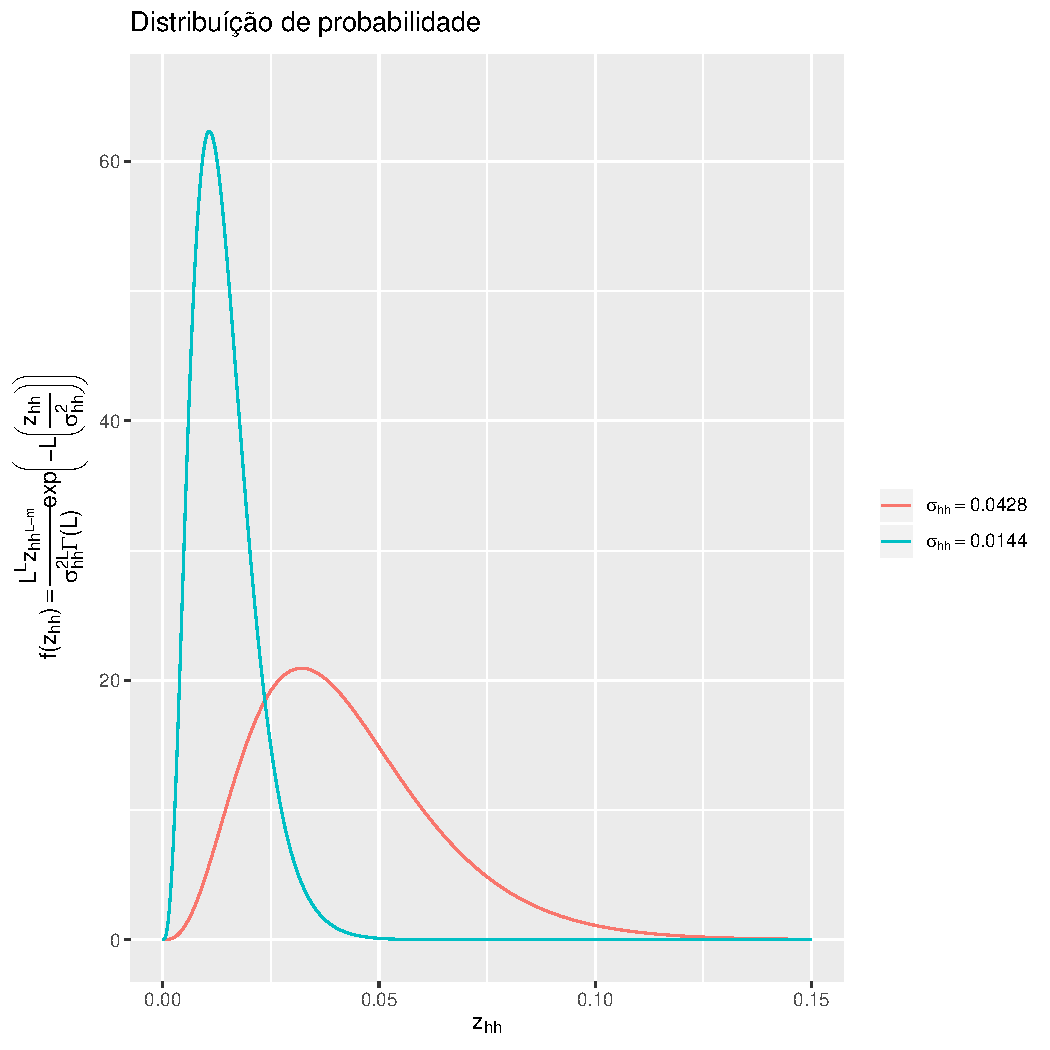
\includegraphics[scale = 1]{grafico_pdf_gamf_2017_sigma_hh.pdf}
  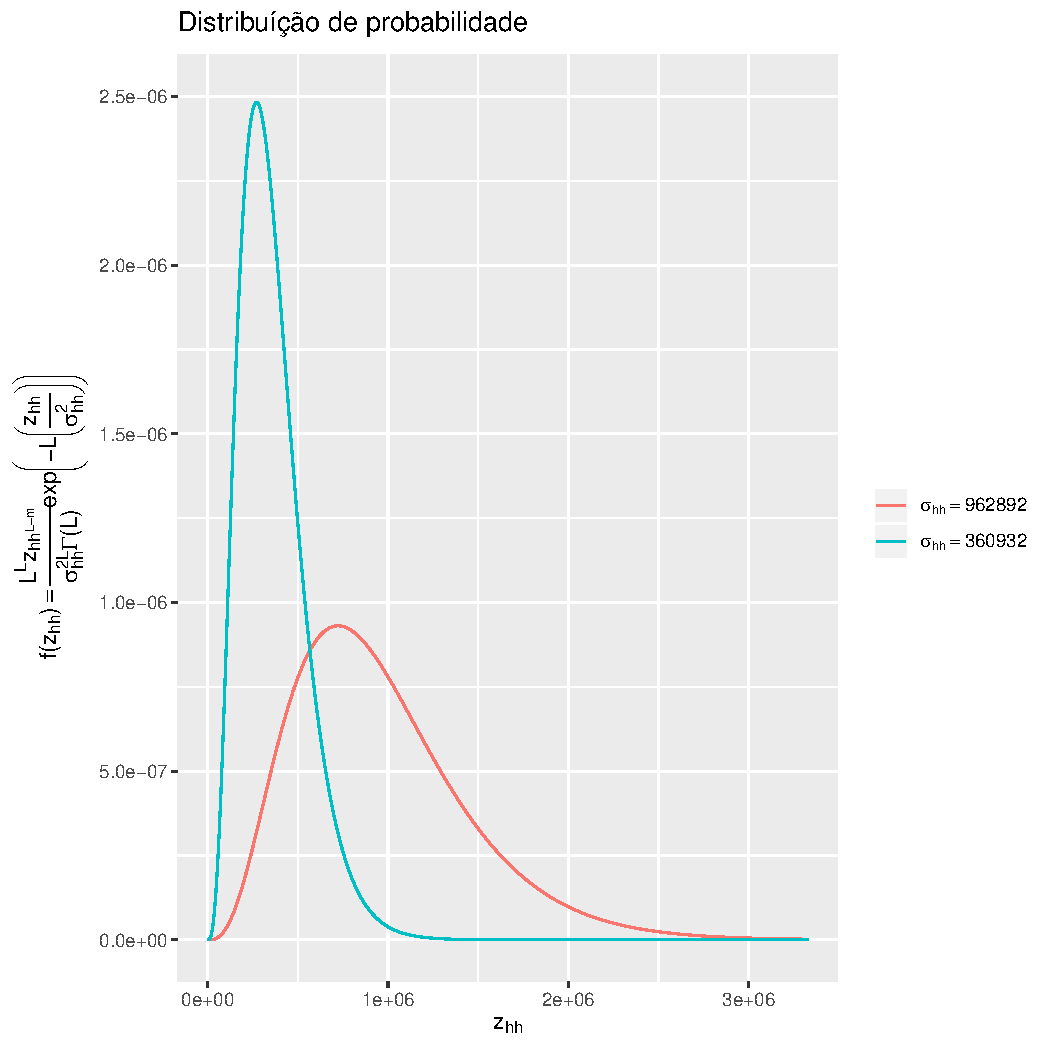
\includegraphics[scale = 0.7]{grafico_pdf_nhfc_2014_sigma_hh.pdf}
	\caption{Funções de densidade para dados simulados.}\label{cap_acf_fig02}
\end{figure}

%\section{Fusão de evidências de bordas}

%	Nesta seção será descrito como realizamos a fusão de evidências de bordas, a referência adotada foi \citet{mit} que mostra várias técnicas de fusão de imagens. 

%	Sejam $I_k(m,n)$, com $k=1,2,\cdots,K$ imagens provenientes da detecção de bordas após a aplicação do método GenSA com dimensões $m \times n$, podemos definir a estratégia de fusão de evidências da seguinte forma, seja o índice $k$ variando como $k=\{hh,vh,vv\}$, para cada linha das imagens e para os respectivos canais $I_k$ temos um valor de evidências de bordas.  Os mesmos serão armazenados em um vetor denotado $ev_k$ com índices variando como $k=\{hh,vh,vv\}$ e dimensão $m$, assim a fusão de evidências $F_{m}^{ev}$ é definida como,
%\begin{equation}\label{cap_acf_27}
%\begin{array}{lll}
%	F_{m}^{ev} &=&\frac{1}{K}\sum_{k=1}^{K}ev_k  \\
%\end{array}
%\end{equation}
% O resultado da técnica de fusão de evidências é mostrado na figura (\ref{cap_acf_fig11}).

%Com o intuito de melhorar a detecção de borda propomos aplicar o método de quadrados mínimos (\textbf{MMQ}) nos dados da fusão de evidências, realizando essa aplicação temos o resultado do método dos quadrados mínimos junto com os pontos de fusão de evidências, mostrados na figura (\ref{cap_acf_fig12}).
%\begin{figure}[hbt]
%\minipage{0.475\textwidth}
%	\fbox{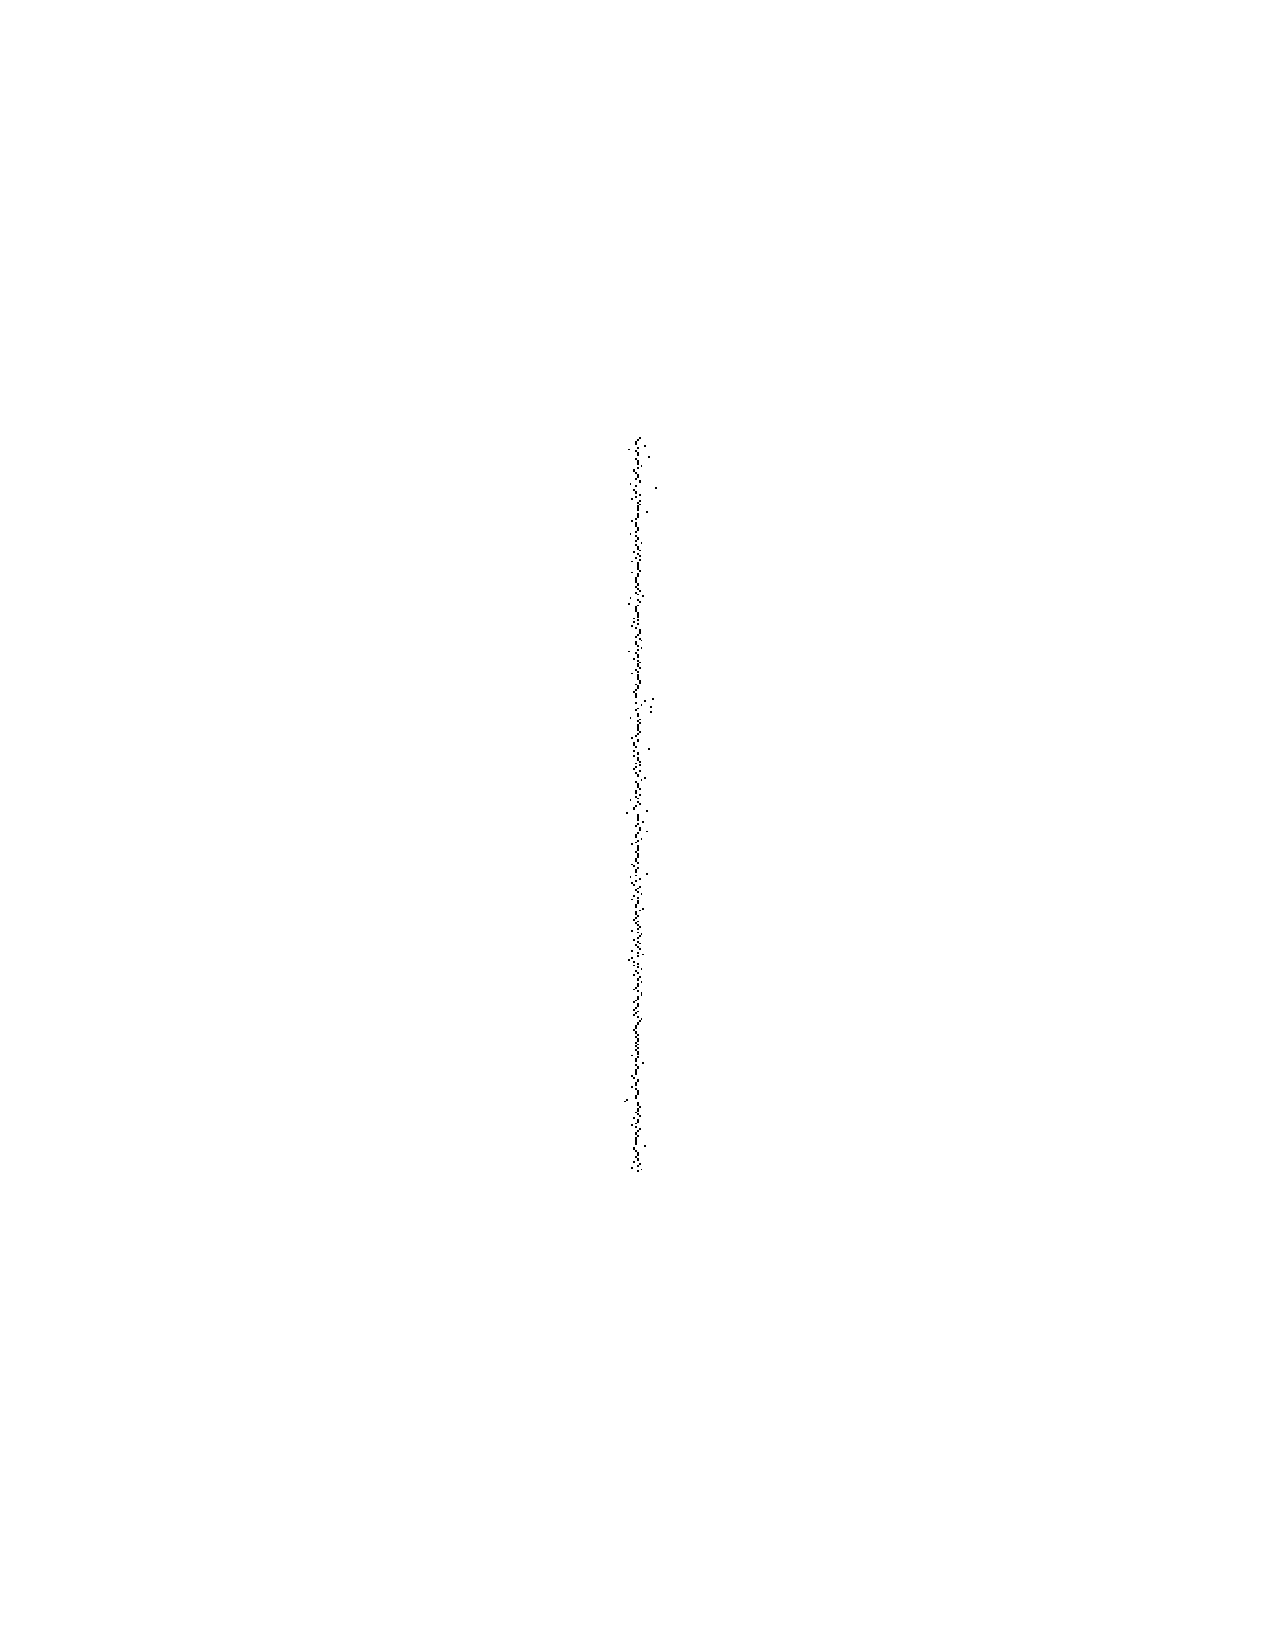
\includegraphics[width=\linewidth]{fusao_soma_ev_hh_hv_vv_nhfc.pdf}}
%	\caption{Fusão de evidências para os canais $\left(I_{hh}, I_{hv}, I_{vv}\right)$.}
%\label{cap_acf_fig11}
%\endminipage\hfill
%\minipage{0.475\textwidth}
%\fbox{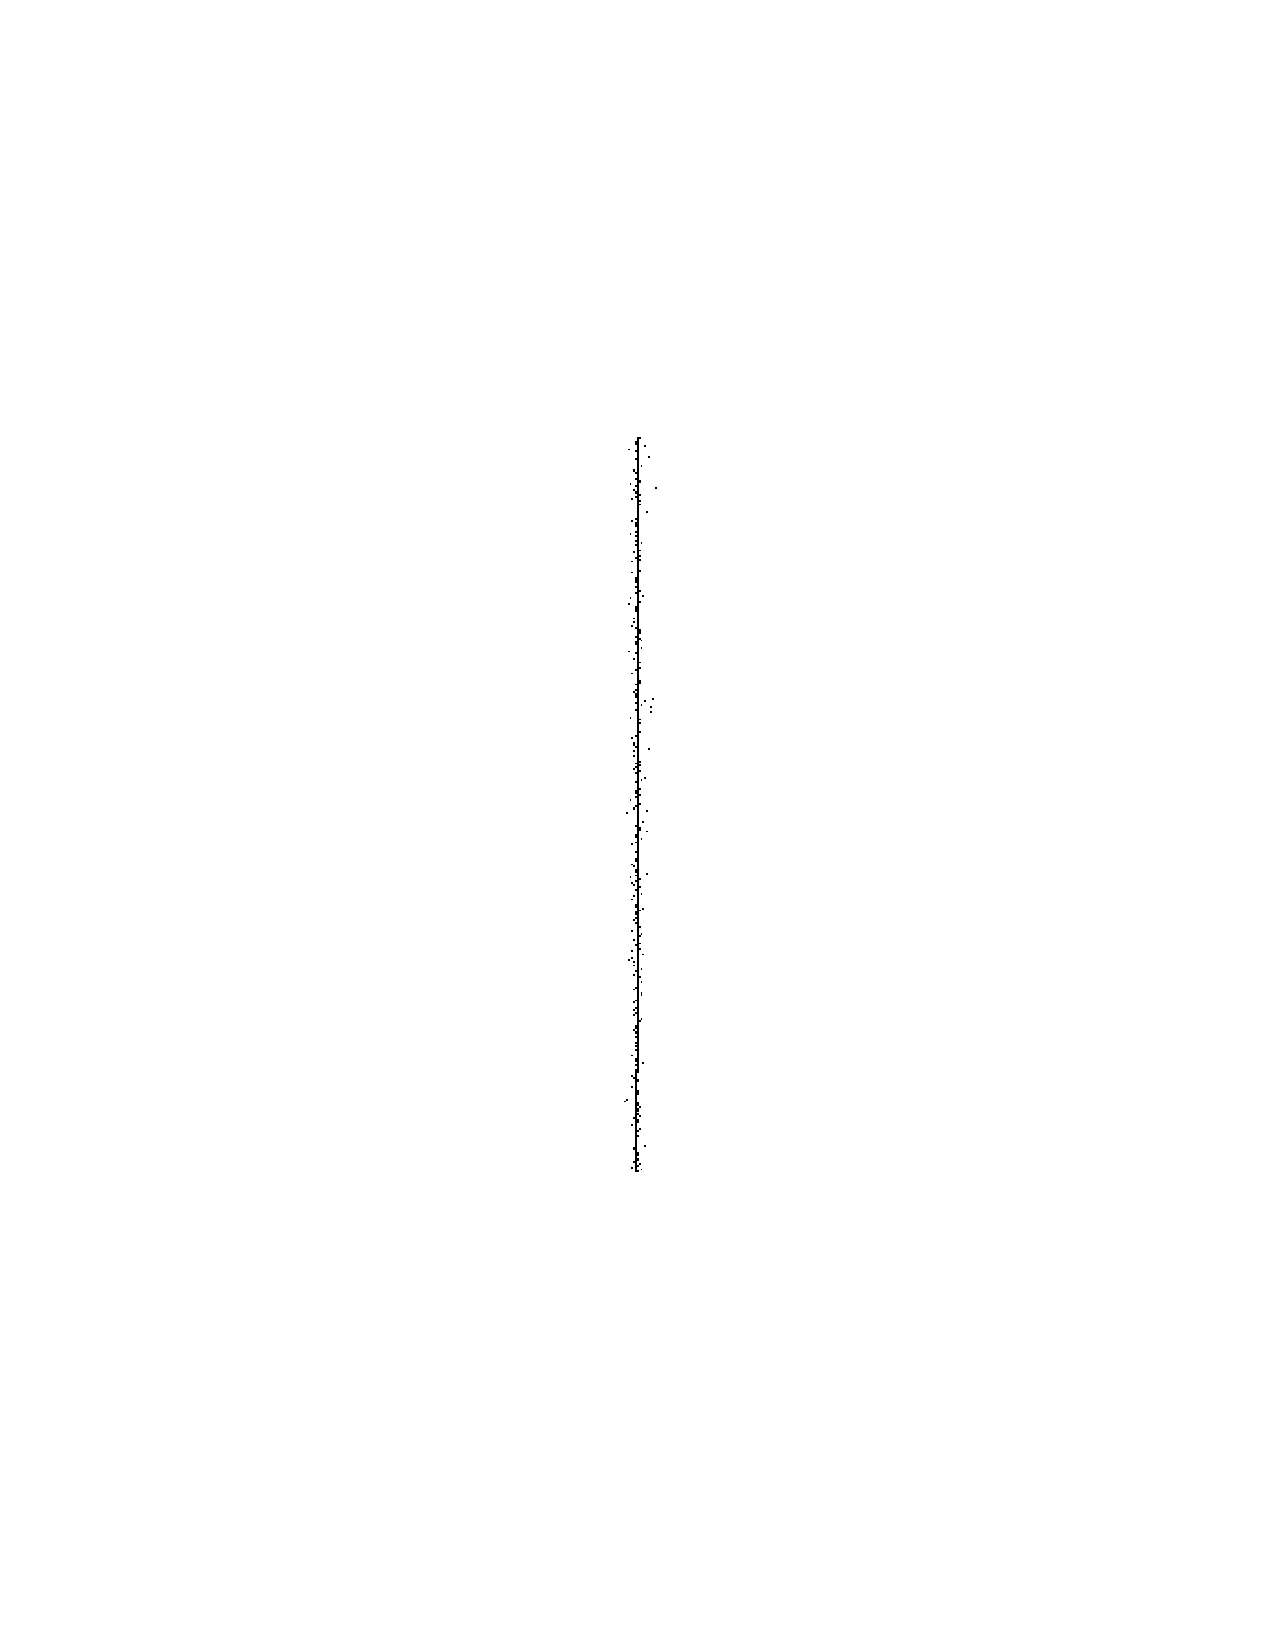
\includegraphics[width=\linewidth]{fusao_ls_nhfc.pdf}}	
%\caption{Método dos quadrados mínimos aplicado a fusão de imagens.}
%\label{cap_acf_fig12}
%\endminipage\hfill
%\end{figure}
%Observando a figura podemos notar um bom desempenho da aplicação do método dos quadrados mínimos nos dados provenientes da fusão de evidências. Para confirmar a observação vamos calcular a frequência relativa desse método, a qual mostra a probabilidade de detecção de borda estimada como na figura (\ref{cap_acf_fig10}).
%\begin{figure}[hbt]
%\minipage{0.475\textwidth}
%	\fbox{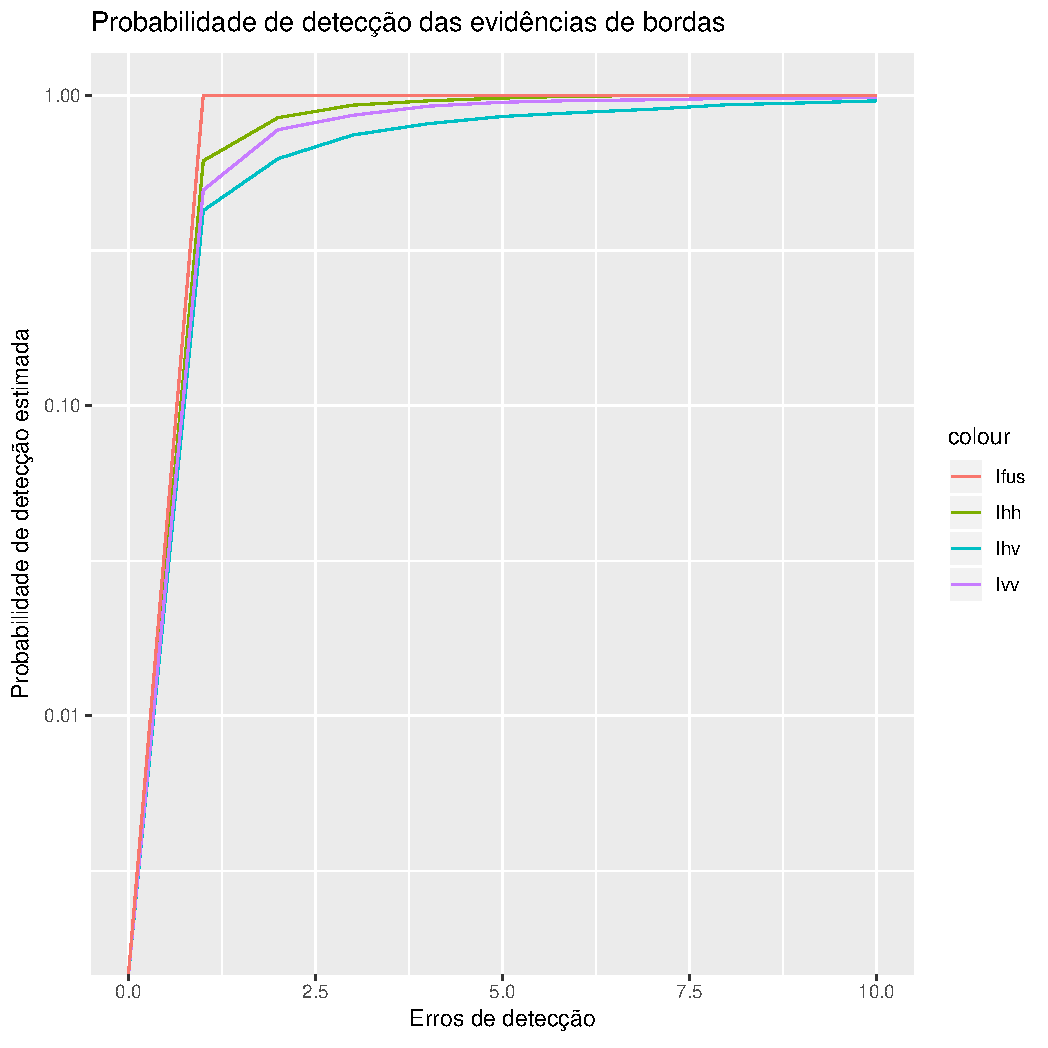
\includegraphics[width=\linewidth]{metricas_ihh_ivh_ivv_ils_nhfc.pdf}}
%	\caption{Probabilidade de detecção de borda com fusão de evidências.}
%\label{cap_acf_fig13}
%\endminipage\hfill
%\minipage{0.475\textwidth}
%\fbox{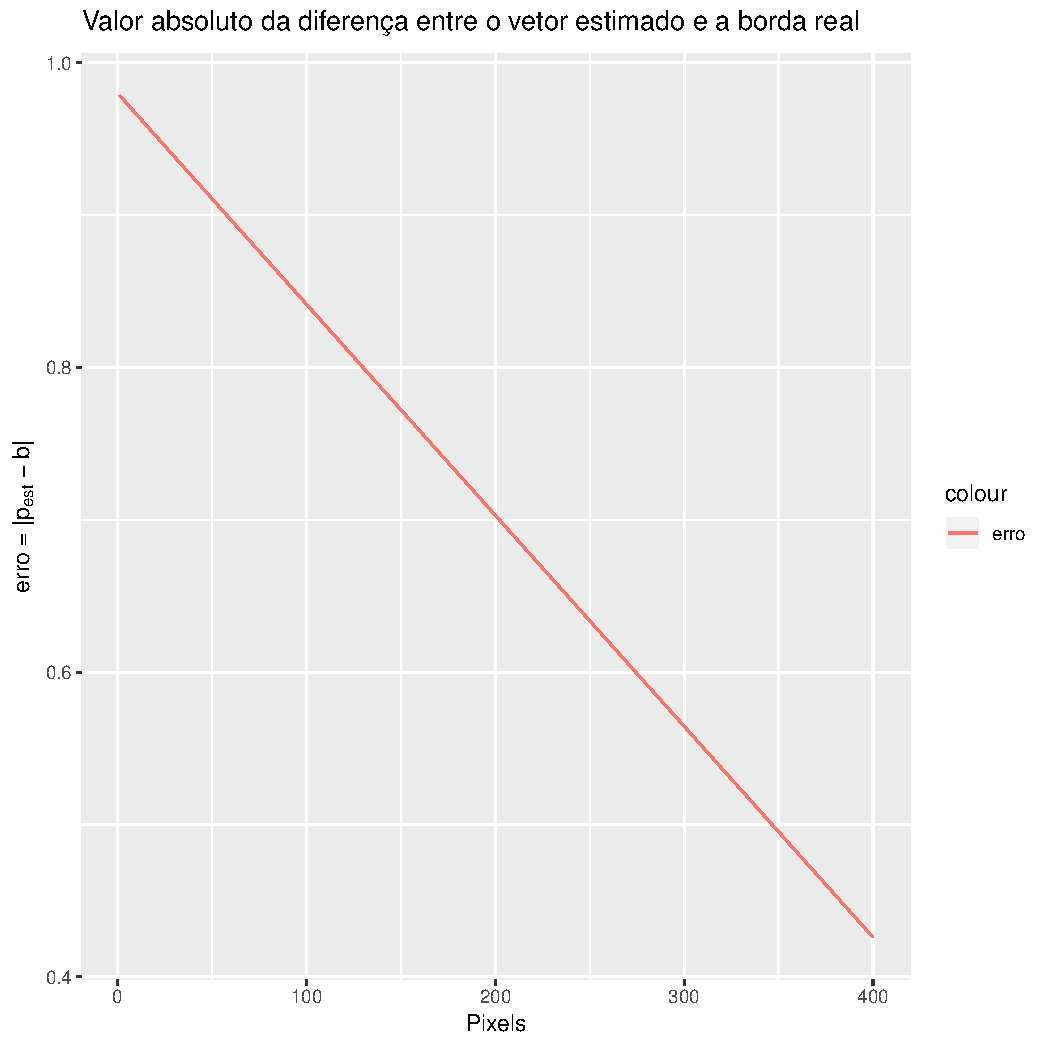
\includegraphics[width=\linewidth]{fusao_ls_erro_nhfc.pdf}}	
%	\caption{Valor absoluto da diferença entre o vetor estimado da fusão de evidências e a borda real.}
%\label{cap_acf_fig14}
%\endminipage\hfill
%\end{figure}

%A figura (\ref{cap_acf_fig13}) mostra a frequência relativa para a fusão de evidências, juntamente com a frequência relativa de detecção de bordas, nos respectivos canais. O gráfico foi construído para notarmos o bom desempenho do método de fusão e posterior aplicação do método dos quadrados mínimos. Desta forma podemos ver que a probabilidade de detecção para o método proposto alcança melhores resultados em relação as detecções em cada canal. 

% Definindo o vetor $P_{est}$ como sendo o vetor de tamanho $400$, tal que, suas componentes são as bordas estimadas pelo método proposto. O vetor $b$ é definido com o valor de borda igual a $200$ para todas as componentes. O gráfico da figura (\ref{cap_acf_fig14}) mostra o $erro=|P_{est}-b|$ para cada pixel que o método foi aplicado, e o máximo atingido do erro foi $erro=0.8162$, isto é, a acurácia do método é menor que um pixel, confirmando o resultado mostrado na figura (\ref{cap_acf_13}).

%A ideia proposta de aplicar o método GenSA para estimar as evidências de bordas juntamente com os métodos de fusão de evidências e quadrados  mínimos (\textbf{MMQ}) teve um desempenho superior na detecção de bordas em relação a detecção nos respectivos canais, como mostra a figura (\ref{cap_acf_fig13}) e (\ref{cap_acf_fig14}). Podemos concluir que para a imagem simulada o método possui uma acurácia satisfatória para a detecção de bordas.
%\chapter{Objetivos}
%Com o propósito de buscar por outros e melhores resultados foram traçados os seguintes objetivos: 
%\begin{itemize}
%    \item[1-] propor e analisar outras técnicas de fusão de evidências (dezembro   2018); 
%	\item[2-] Aplicar o método em uma imagem real para analisar o seu desempenho e acurácia borda encontrada (março 2019);
%	\item[3-] Propor e analisar outras técnicas de regressão ou classificação como por exemplo Support Vector Machine $(SVM)$, ou Randon Forest $(RF)$ para  comparar com o método de quadrados mínimos usado neste texto (março 2019);
%	\item[4-] Aplicar um filtro tipo borrador na função $l(j)$ com intuito de melhorar sua suavidade facilitando o cálculo do gradiente e consequentemente comparar métodos clássicos de otimização com a aplicação do método GenSA proposto neste trabalho (dezembro 2018). 
%\end{itemize}

%Propostas para \textit{workshops}, congressos e publicações:
%\begin{itemize}
%\item participar do \textit{workshop} semestral promovido pelo programa de pós-graduação em engenharia elétrica e computação (dezembro 2018);
%\item finalizar um artigo para publicar em congresso de relevância internacional (dezembro 2018);
%\item finalizar um artigo para publicar em revista internacional avaliada de acordo com a área de atuação (março 2019);
%\end{itemize}
%\chapter{Testes numéricos}
\section{Sigmas do artigo }
\begin{equation}\label{matriz_sigma_gamf_1}
	\hspace{2.75cm} \Sigma_{u}= \left[
\begin{array}{lll}
0.042811            & 0.000072-0.003180i & 0.010435+0.005022i\\
0.000072+0.003180i  & 0.035977           & 0.000784+0.004886i\\
0.010435-0.005022i  & 0.000784-0.004886i & 0.066498
\end{array}
\right],
\end{equation}
\begin{equation}\label{matriz_sigma_gamf_2}
 \Sigma_{f}= \left[
\begin{array}{lll}
0.014380            & 0.001333-0.000076i & -0.000755+0.001570i\\
0.001333+0.000076i  & 0.002789           & -0.001044+0.001101i\\
-0.000755-0.001570i &-0.001044-0.001101i & 0.015387
\end{array}
\right],
\end{equation}

%S(:,:,2)= [ 
%0.042811  0.000072+-0.003180i 0.010435+0.005022i
%0.000072+0.003180i 0.035977 0.000784+0.004886i
%0.010435+-0.005022i 0.000784+-0.004886i 0.066498];

% Class:
%S(:,:,2) = [ 
%0.014380  0.001333+-0.000076i -0.000755+0.001570i
%0.001333+0.000076i 0.002789 -0.001044+0.001101i
%-0.000755+-0.001570i -0.001044+-0.001101i 0.015387];



\begin{figure}[hbt]
\centering
	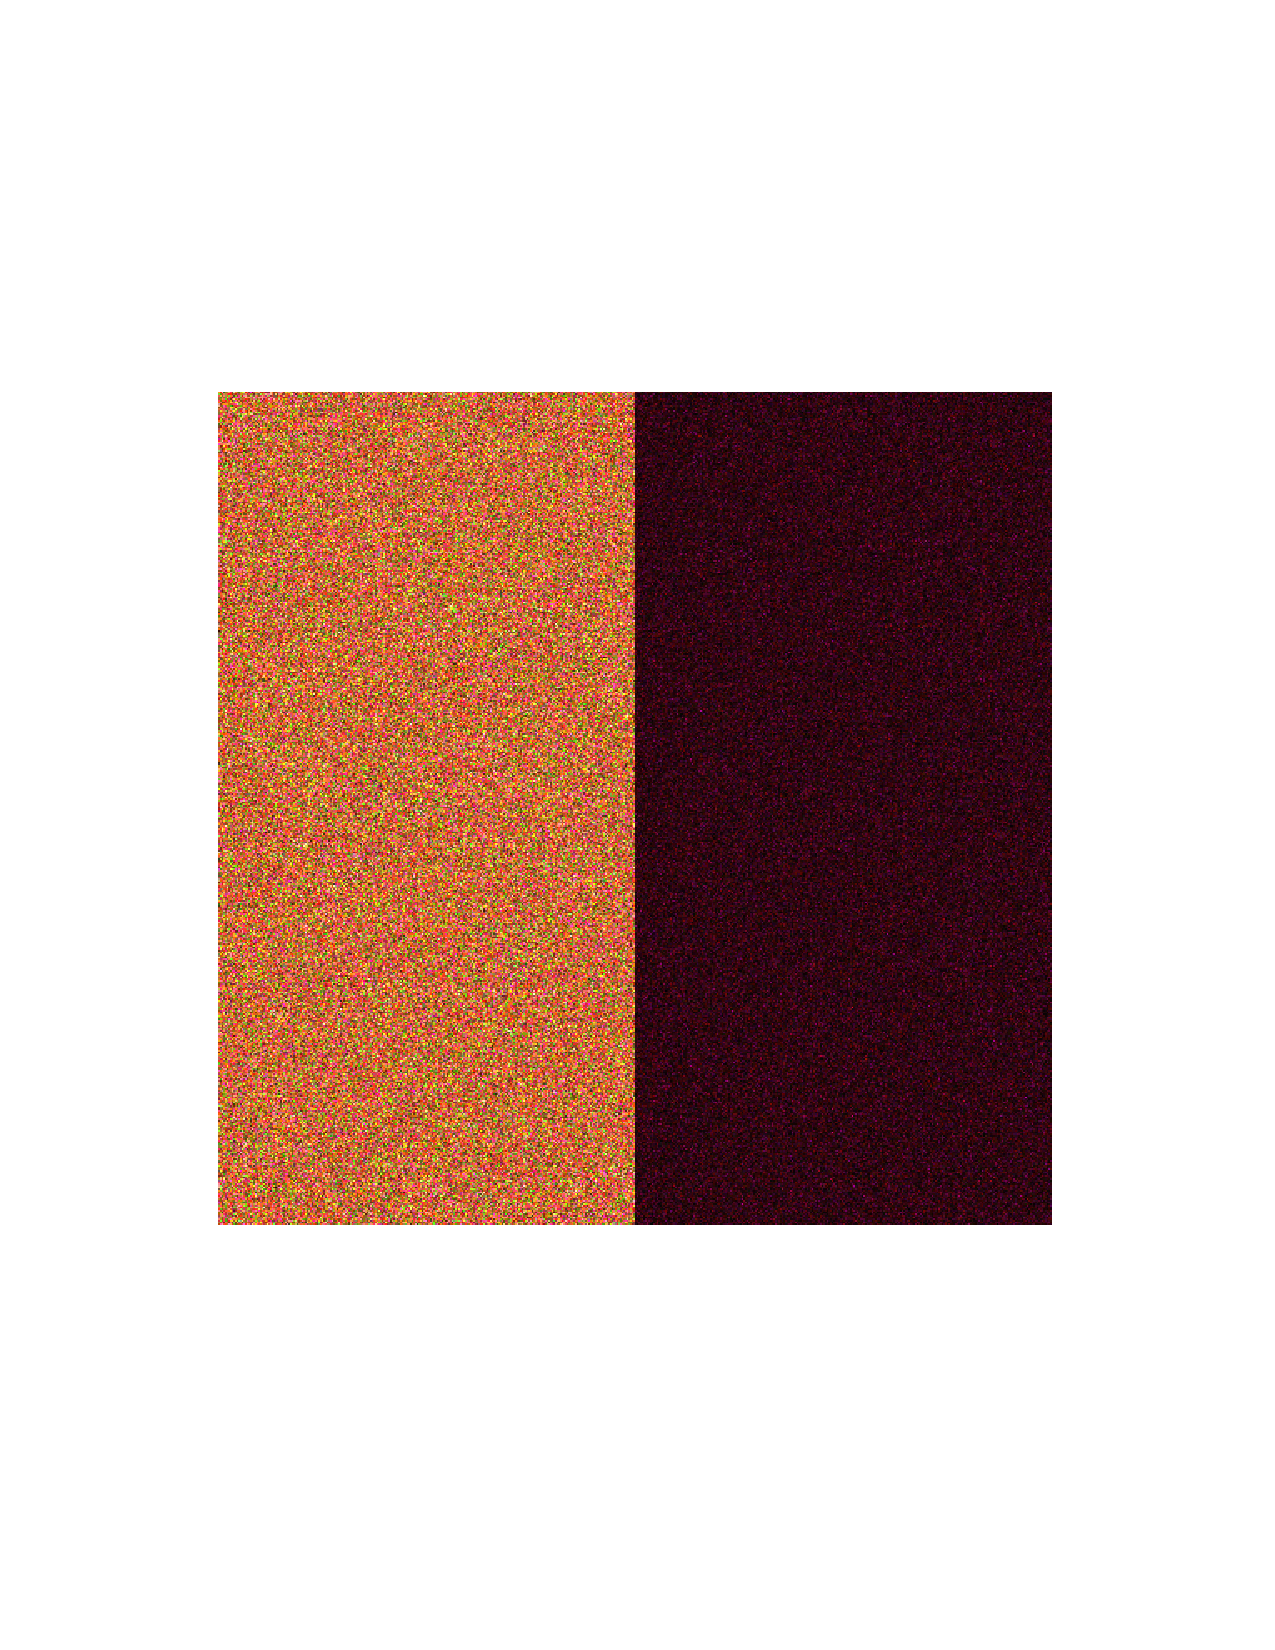
\includegraphics[width=5.0in]{phanton_gamf_dec_pauli.pdf}
	\caption{Decomposição de Pauli uma das phantons com valores de $\Sigma$ propostos no artigo \citep{gamf}.}\label{cap_acf_fig01}
\end{figure}
\begin{figure}[hbt]
	\centering
	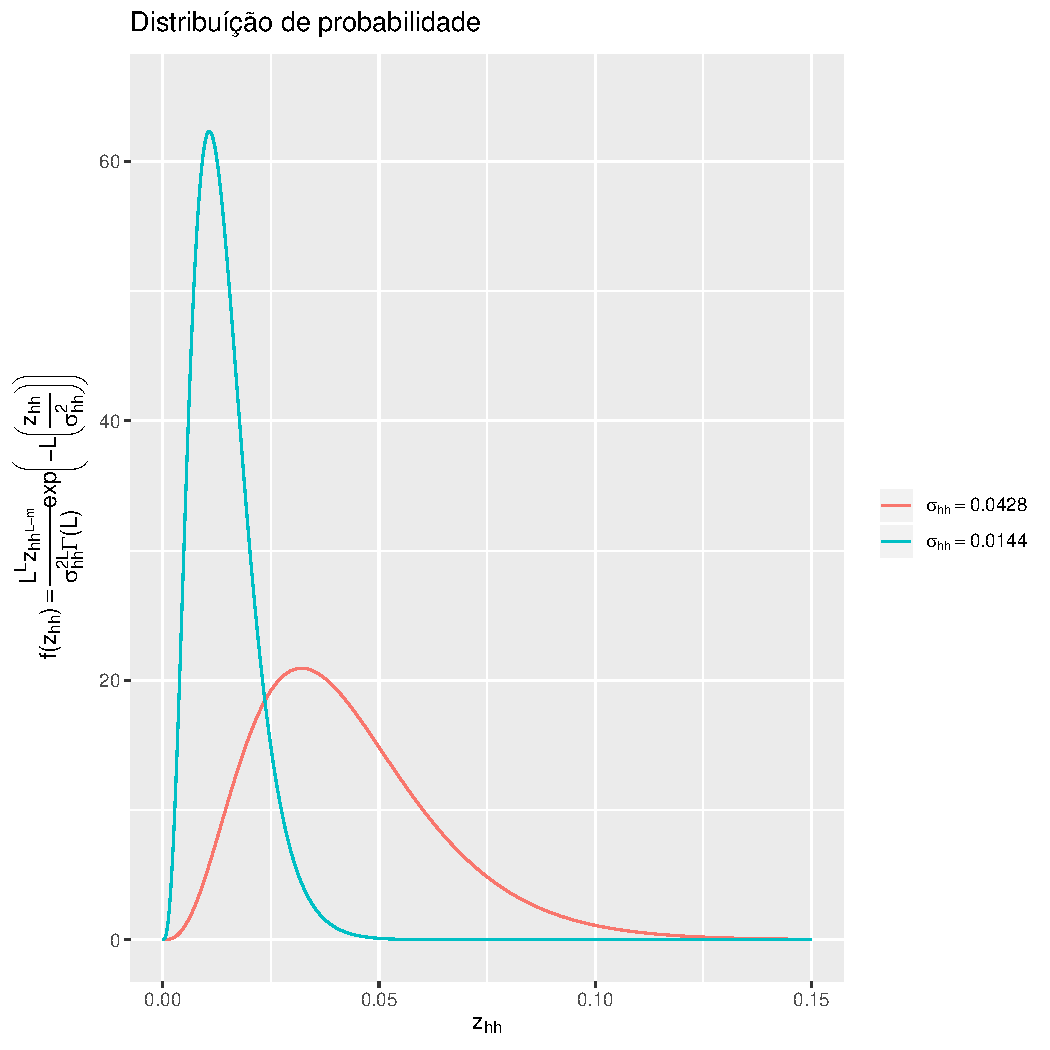
\includegraphics[scale = 0.7]{grafico_pdf_gamf_2017_sigma_hh.pdf}
	\caption{Funções de densidade para dados simulados.}\label{cap_acf_fig02}
\end{figure}

\begin{figure}[hbt]
\minipage{0.5\textwidth}
  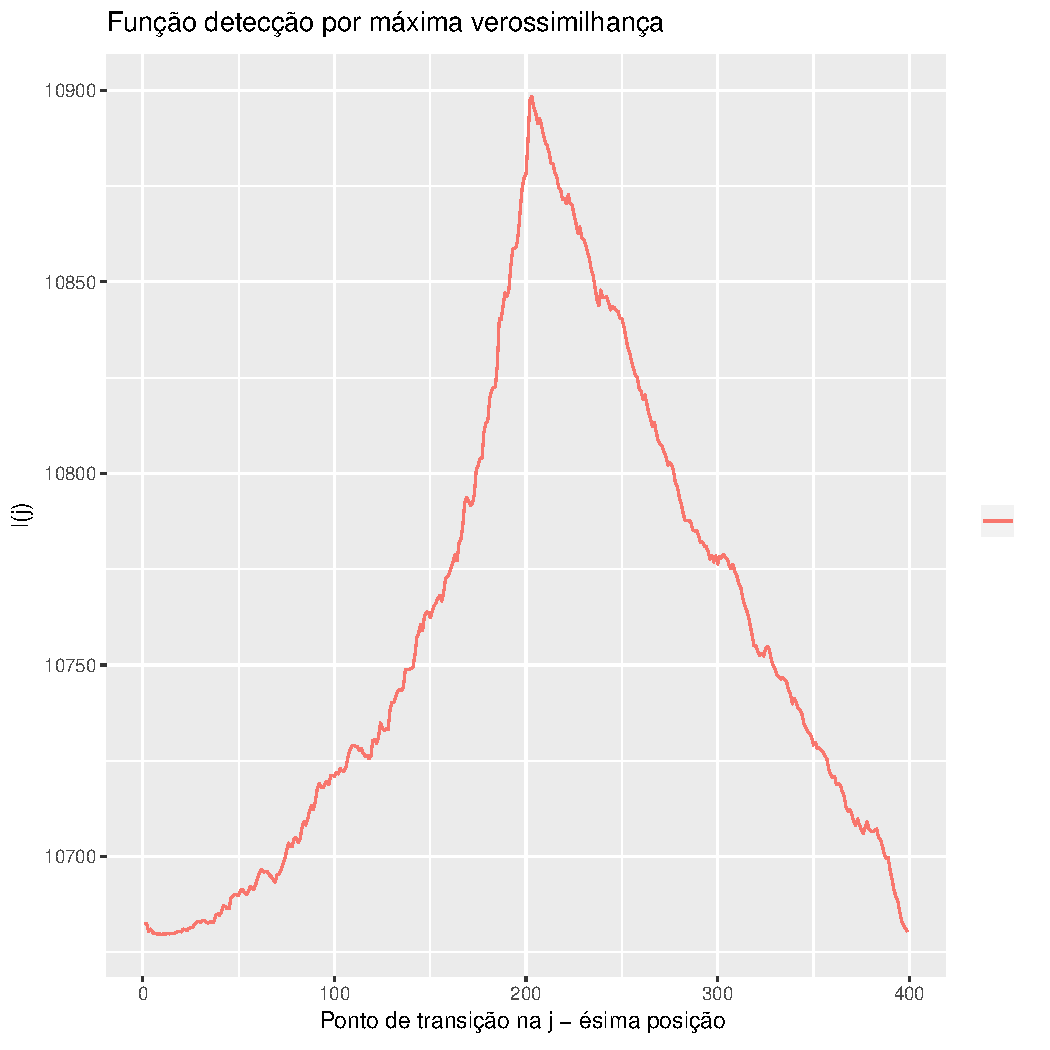
\includegraphics[width=\linewidth]{grafico_l_gamf_2017_sigmahh.pdf}
	\caption{Função $l(j)$ para o canal $I_{HH}$}\label{cap_acf_fig04}
\endminipage\hfill
\minipage{0.5\textwidth}
  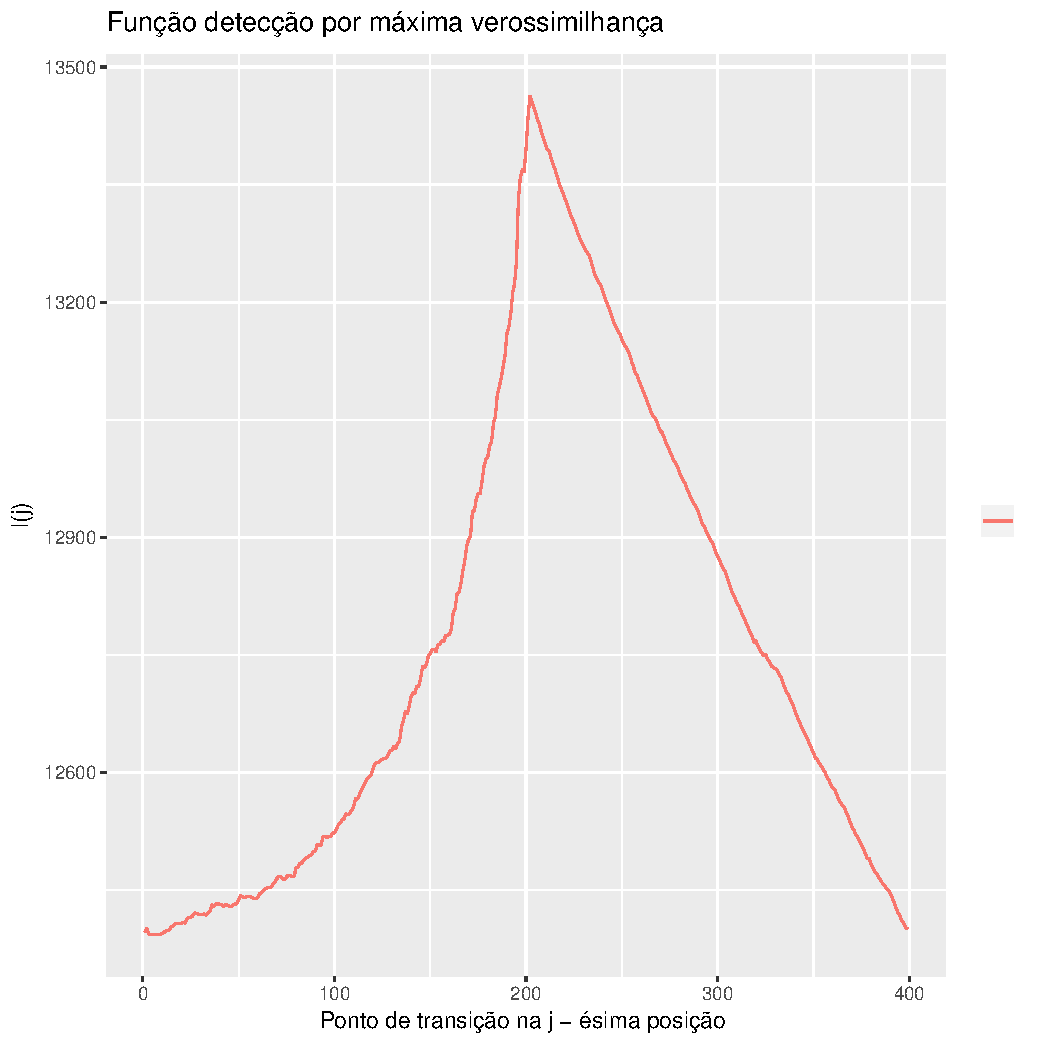
\includegraphics[width=\linewidth]{grafico_l_gamf_2017_sigmahv.pdf}
	\caption{Função $l(j)$ para o canal $I_{HV}$}\label{cap_acf_fig05}
\endminipage\hfill
\centering
\minipage{0.5\textwidth}
  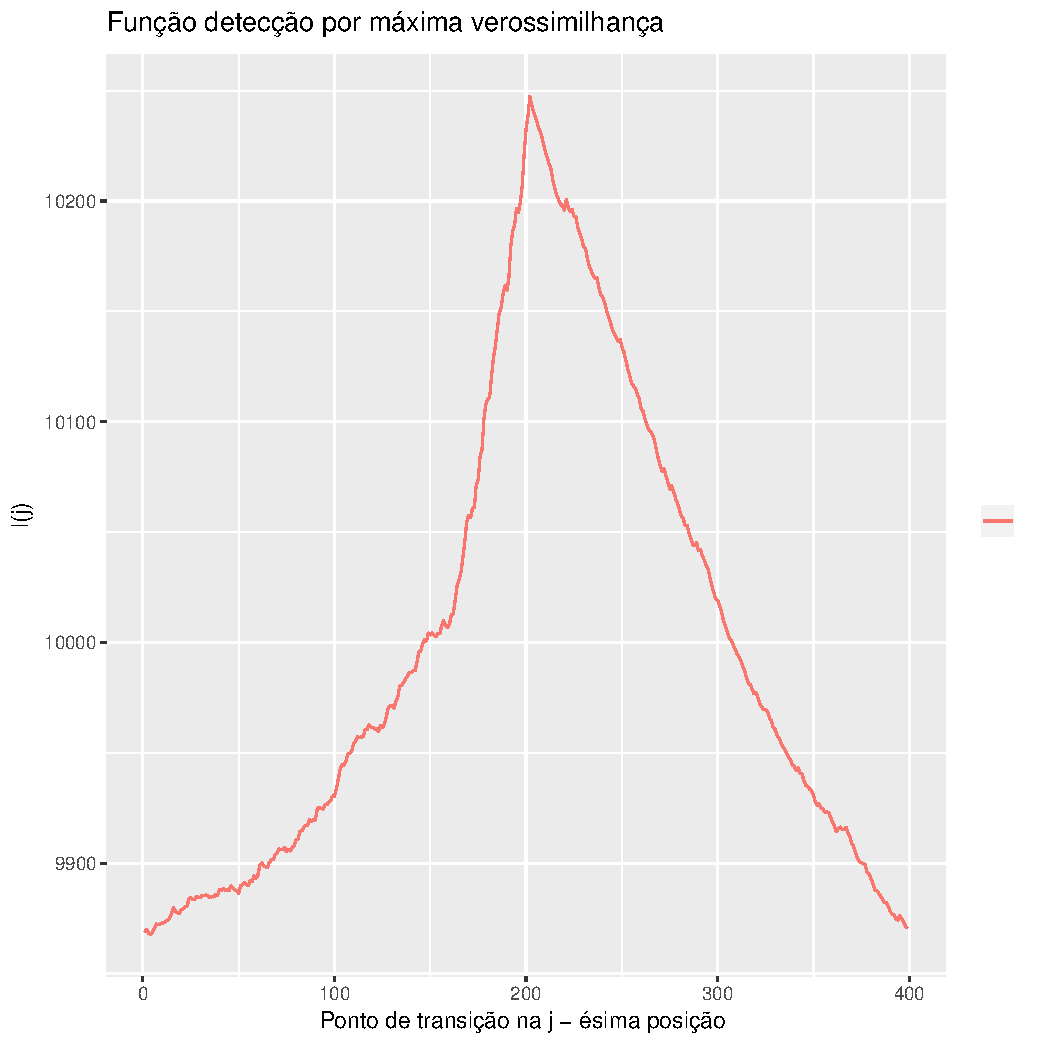
\includegraphics[width=\linewidth]{grafico_l_gamf_2017_sigmavv.pdf}
	\caption{Função $l(j)$ para o canal $I_{VV}$}\label{cap_acf_fig06}
\endminipage\hfill
\end{figure}
\begin{figure}[hbt]
\minipage{0.475\textwidth}
\fbox{  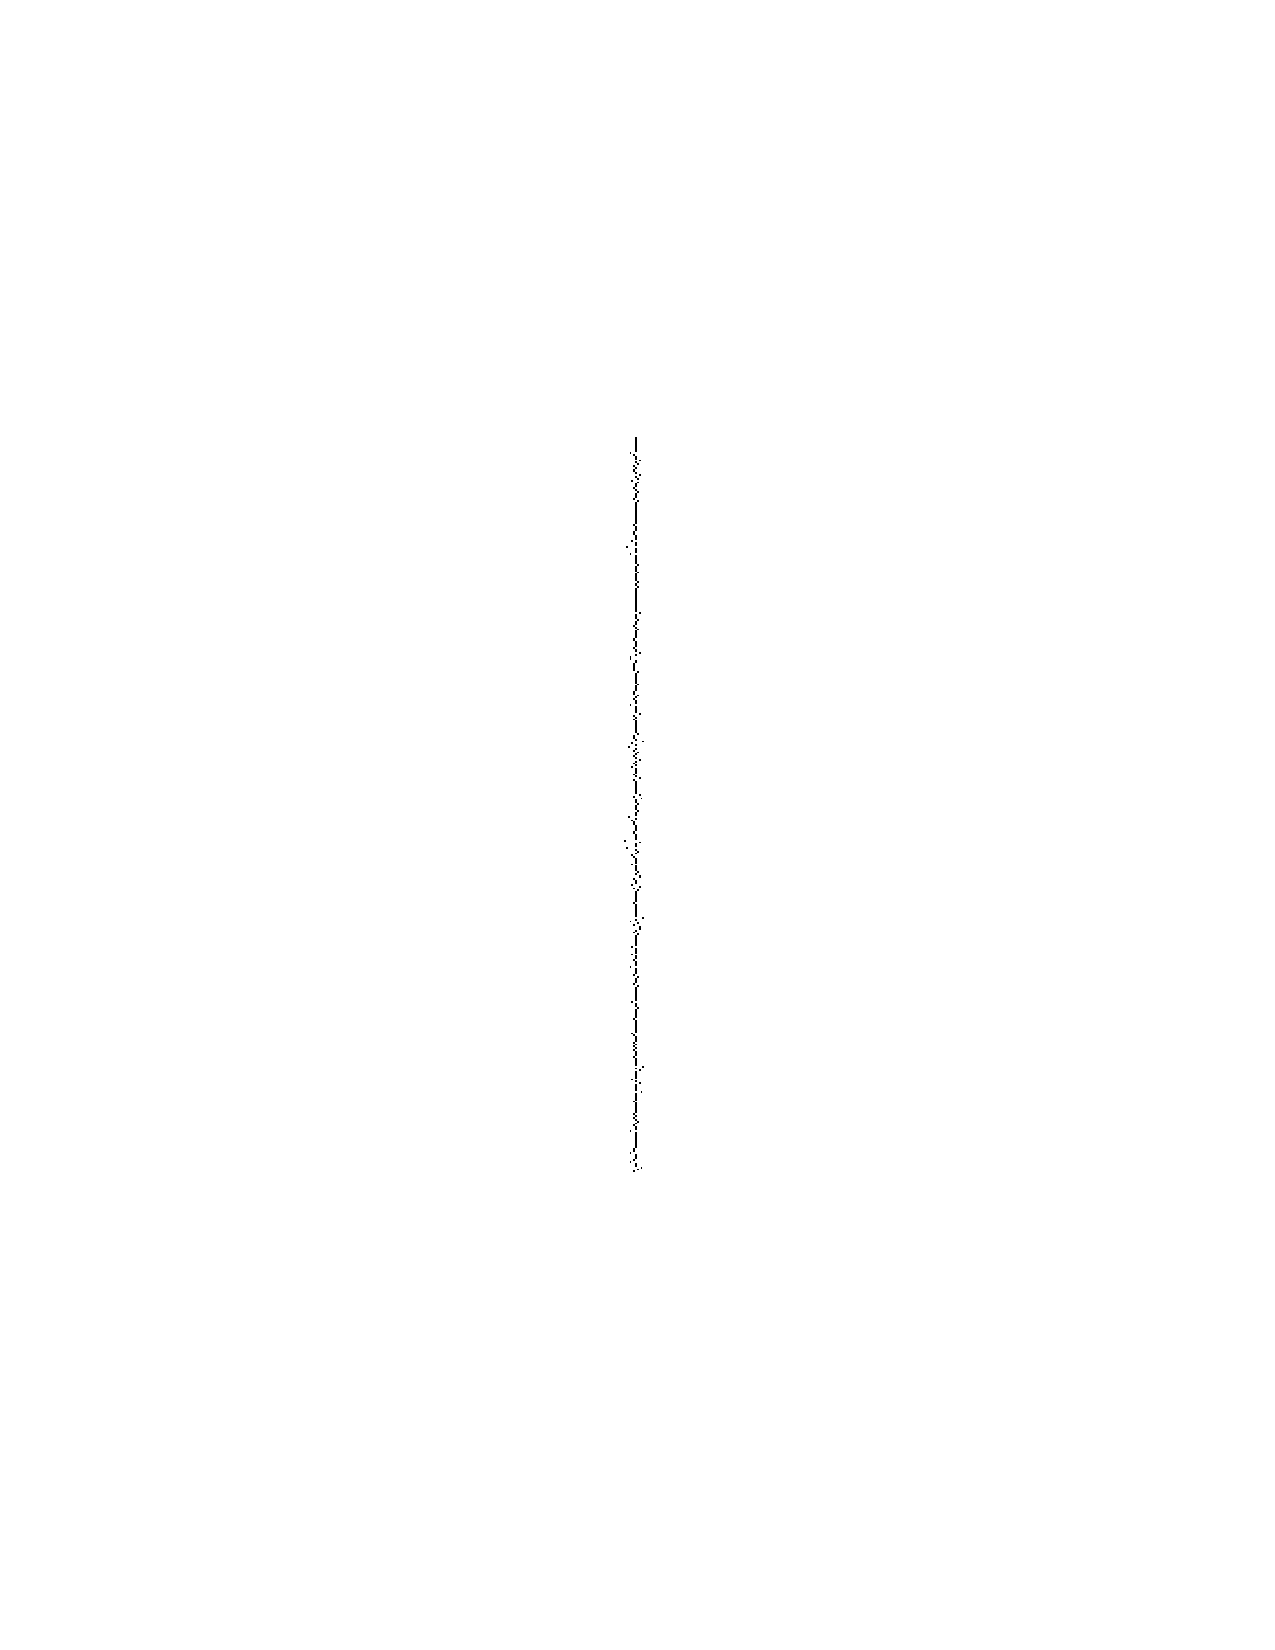
\includegraphics[width=\linewidth]{ev_hh_gamf_2017.pdf}}
\caption{Evidências de bordas para o canal $I_{HH}$}\label{cap_acf_fig07}
\endminipage\hfill
\minipage{0.475\textwidth}
\fbox{ 
\includegraphics[width=\linewidth]{ev_hv_gamf_2017.pdf}}
\caption{Evidências de bordas para o canal $I_{HV}$}\label{cap_acf_fig08}
\endminipage\hfill
\centering
\minipage{0.475\textwidth}
\fbox{ 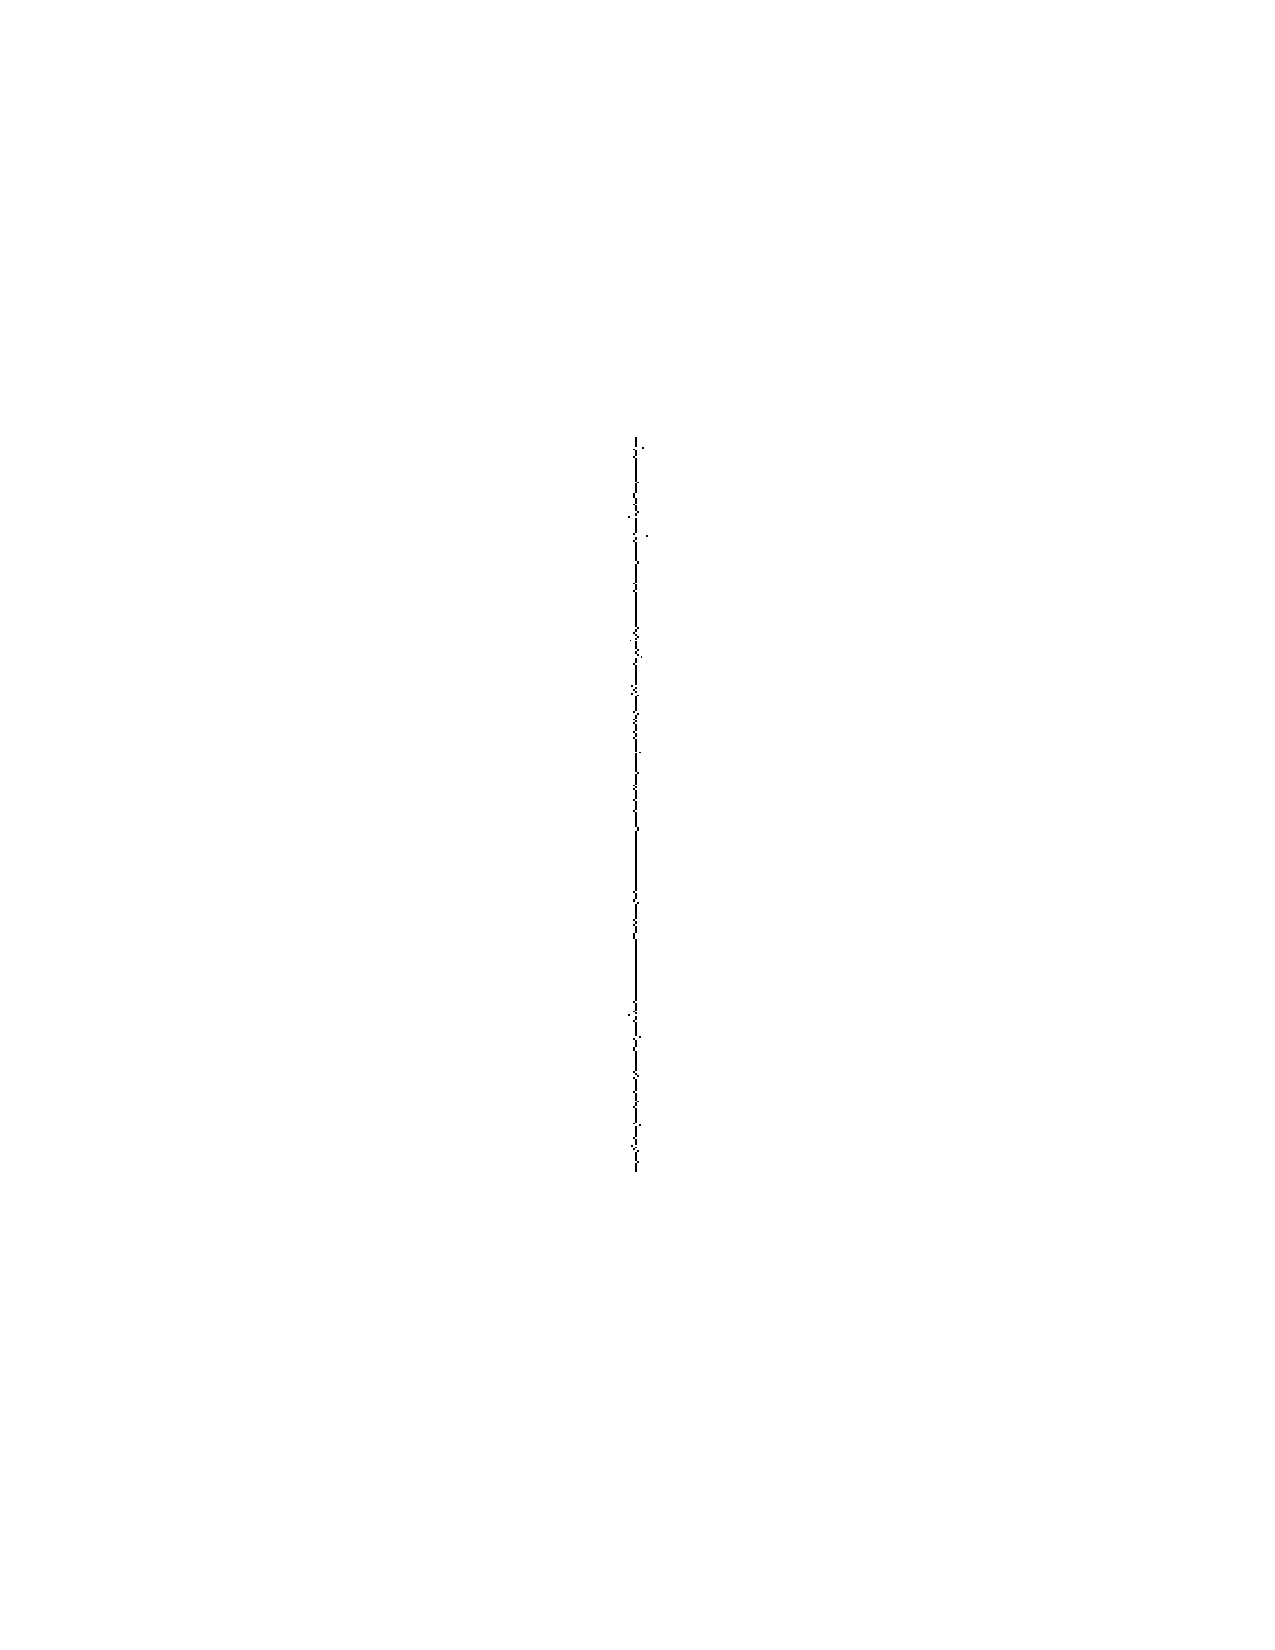
\includegraphics[width=\linewidth]{ev_vv_gamf_2017.pdf}}
\caption{Evidências de bordas para o canal $I_{VV}$}\label{cap_acf_fig09}
\endminipage\hfill
\end{figure}
%
\begin{figure}[hbt]
\centering
	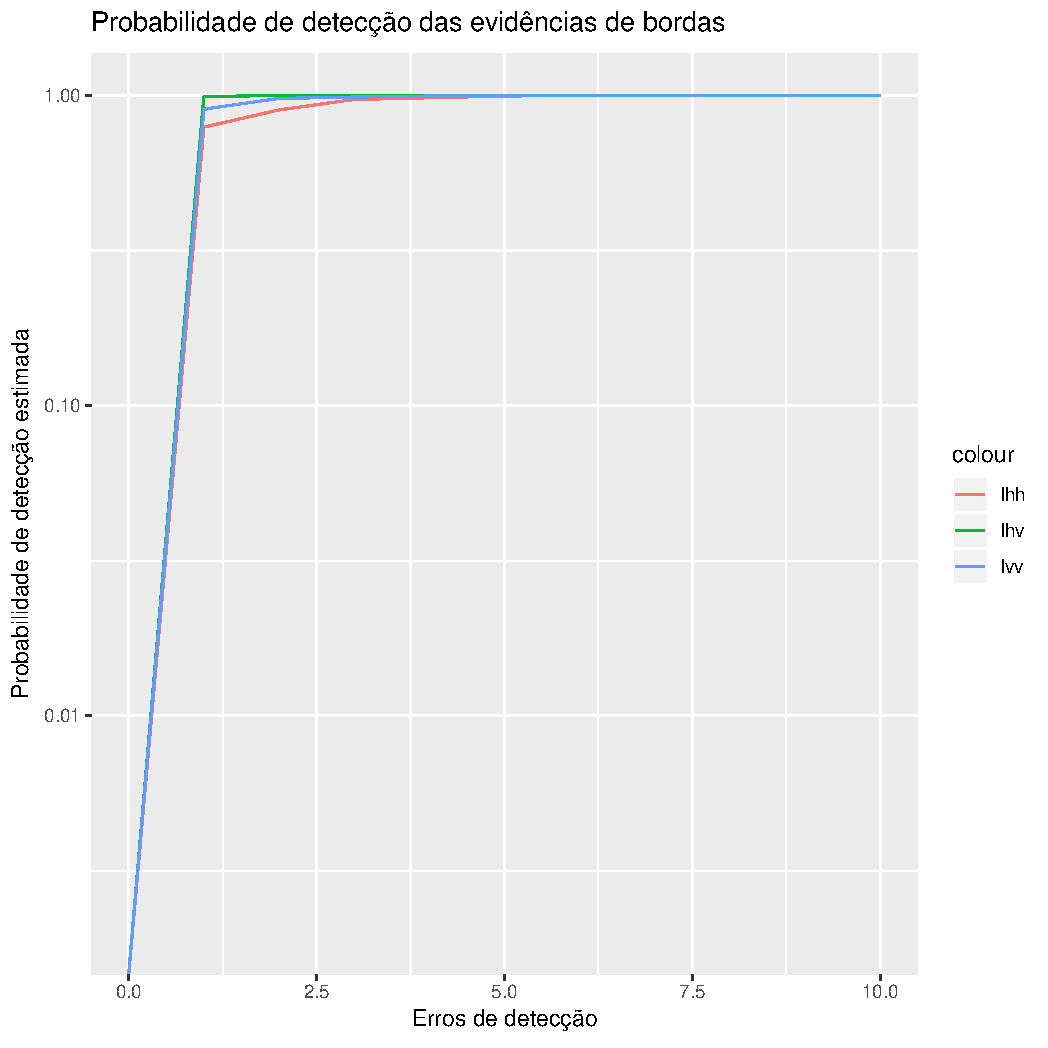
\includegraphics[width=5.0in]{metricas_ihh_ivh_ivv_gamf.pdf}
	\caption{Probabilidade de detecção de borda estimada usando GenSA.}
\label{cap_acf_fig10}
\end{figure}
%
%\begin{figure}[hbt]
%\minipage{0.475\textwidth}
%	\fbox{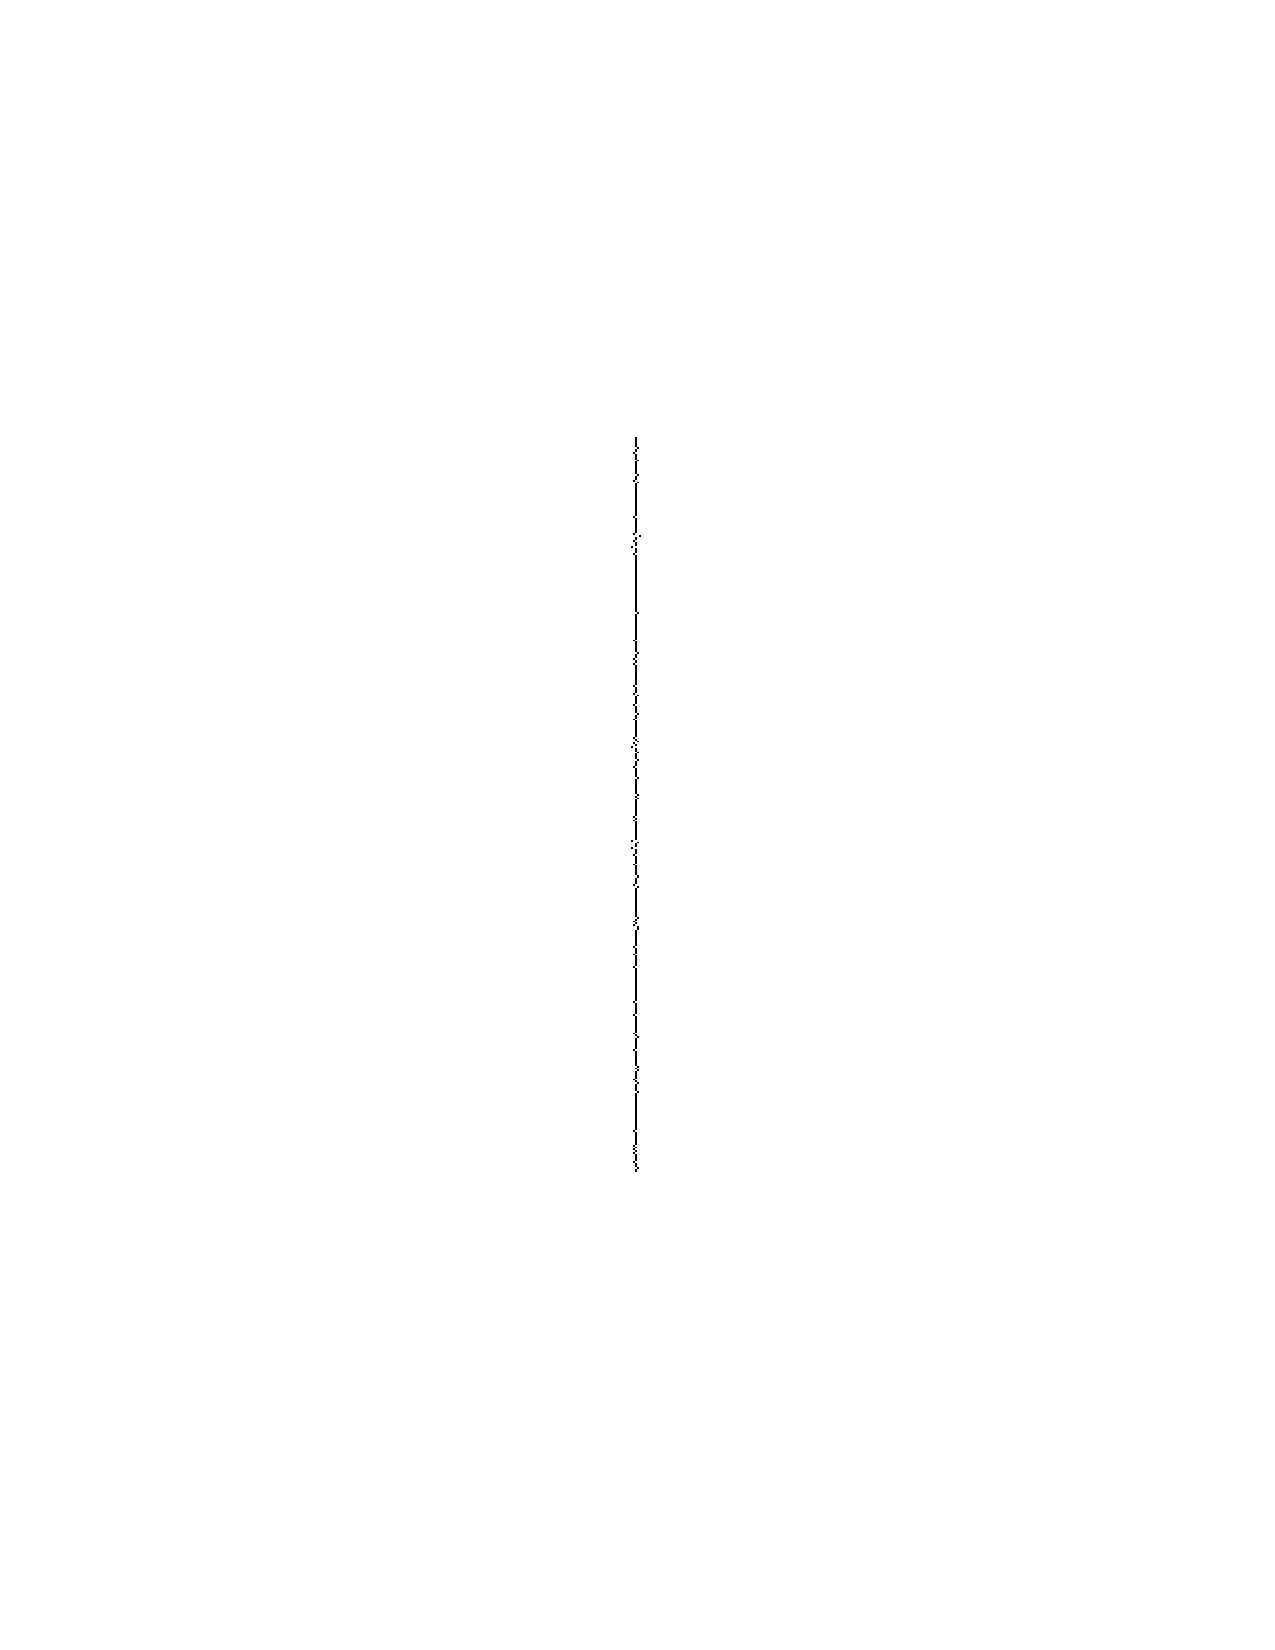
\includegraphics[width=\linewidth]{fusao_soma_ev_hh_hv_vv_gamf.pdf}}
%	\caption{Fusão de evidências para os canais $\left(I_{hh}, I_{hv}, I_{vv}\right)$.}
%\label{cap_acf_fig11}
%\endminipage\hfill
%\minipage{0.475\textwidth}
%\fbox{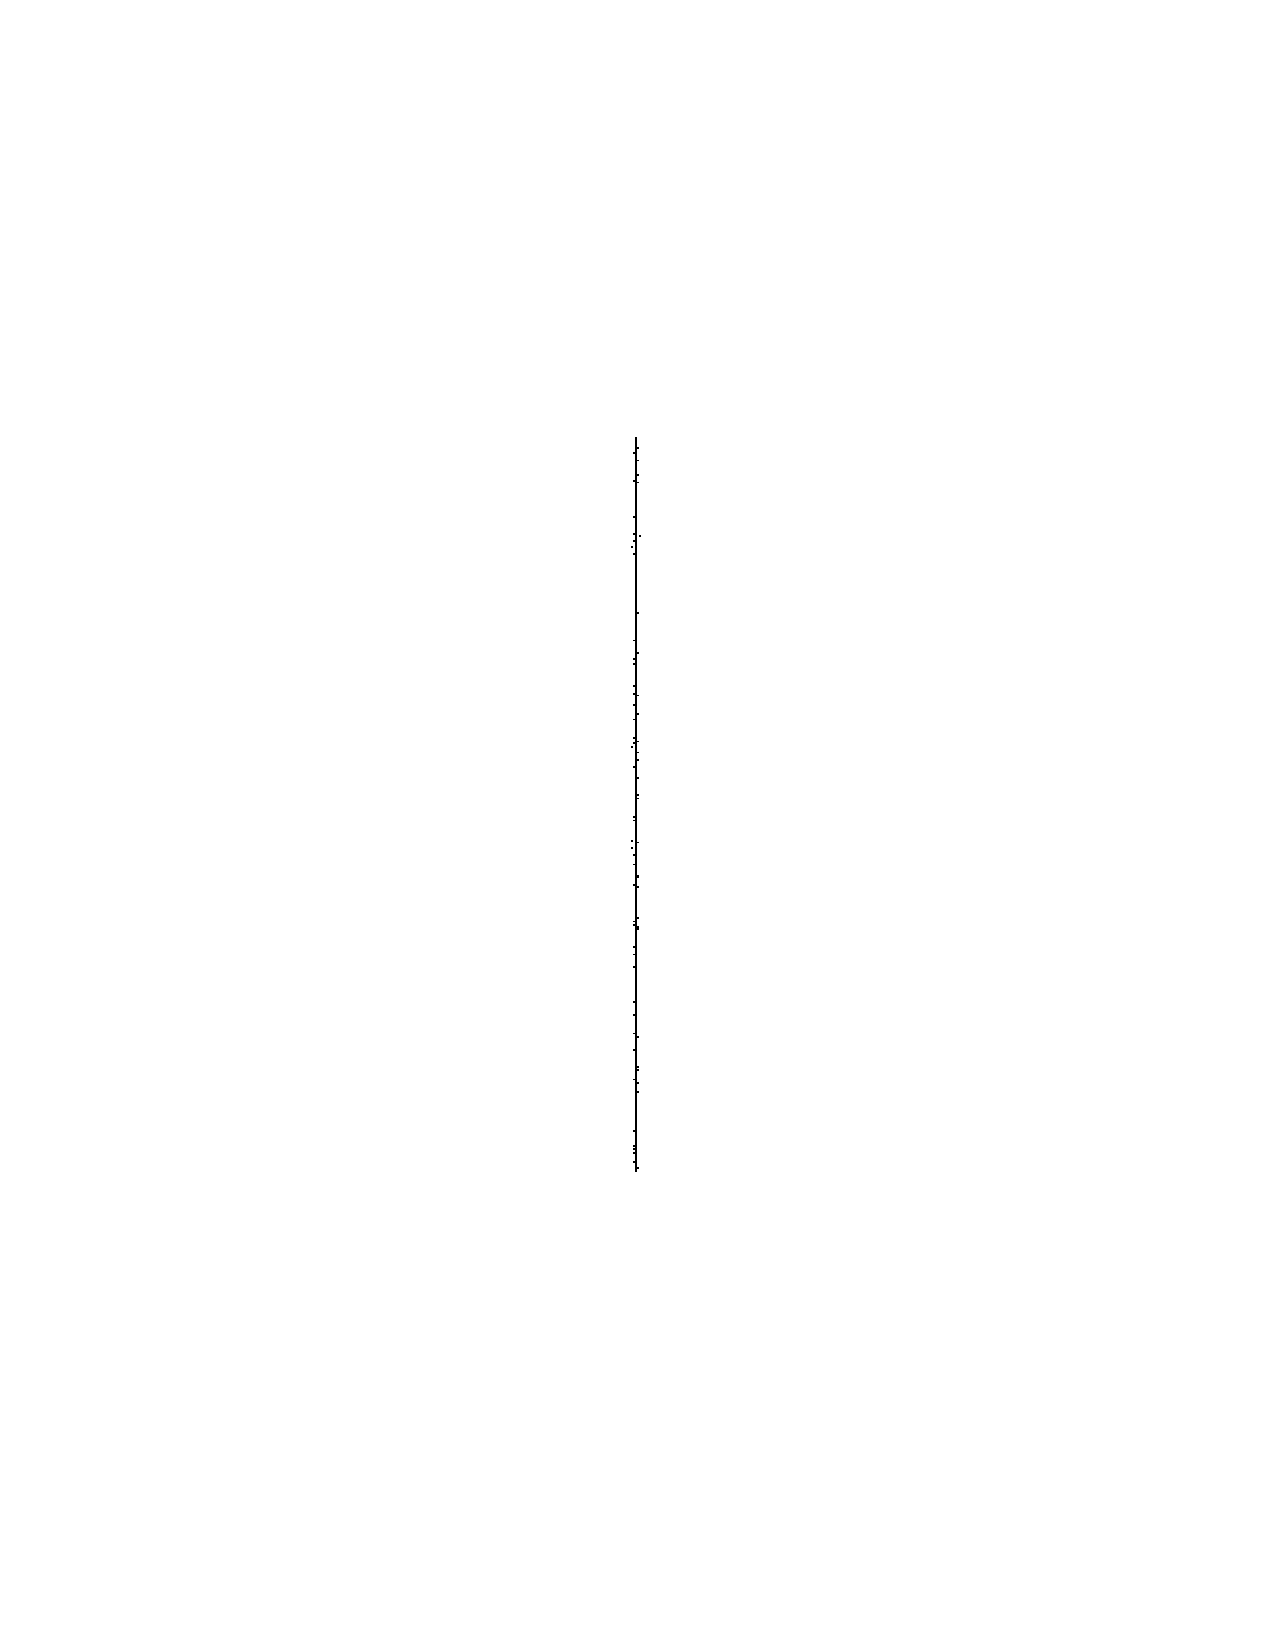
\includegraphics[width=\linewidth]{fusao_ls_gamf.pdf}}	
%\caption{Método dos quadrados mínimos aplicado a fusão de imagens.}
%\label{cap_acf_fig12}
%\endminipage\hfill
%\end{figure}
%\begin{figure}[hbt]
%\minipage{0.475\textwidth}
%	\fbox{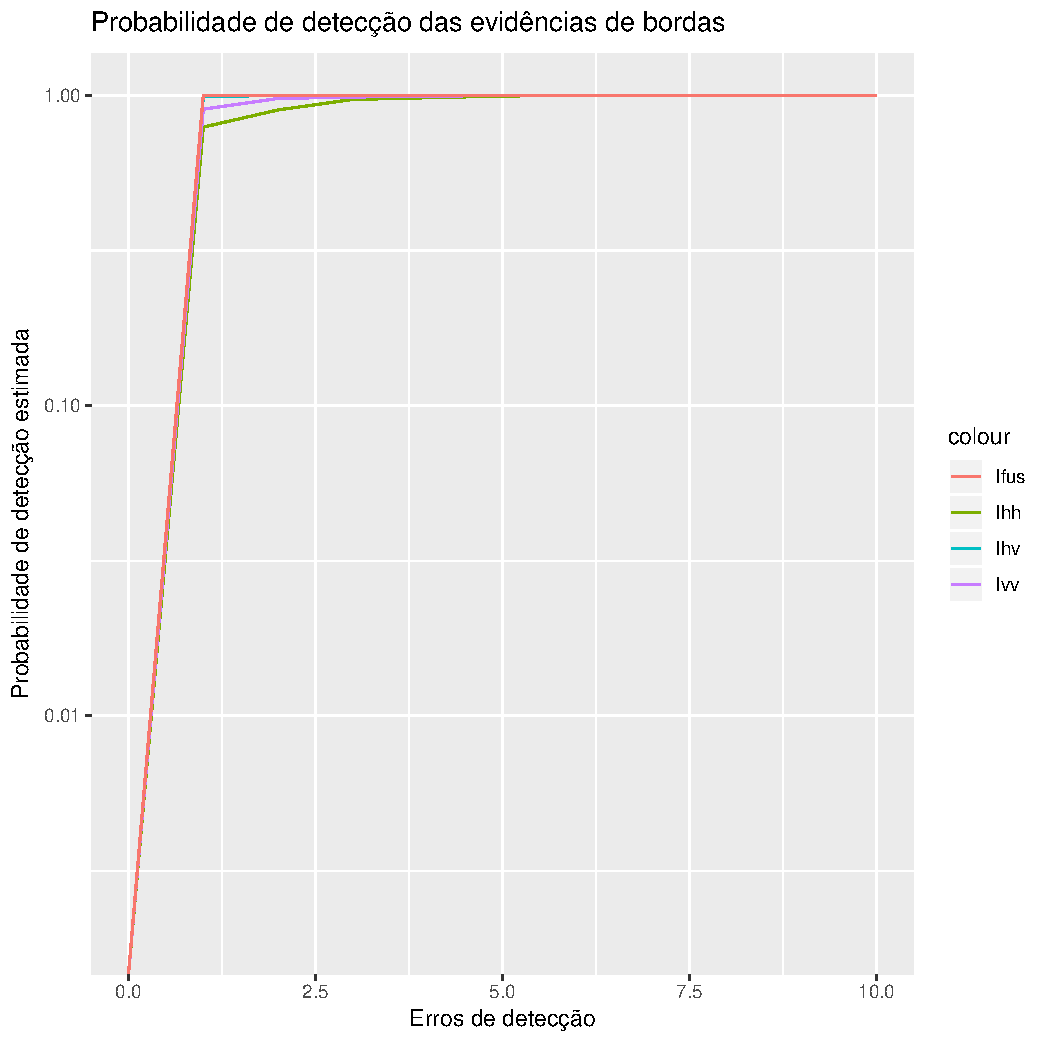
\includegraphics[width=\linewidth]{metricas_ihh_ivh_ivv_ils_gamf.pdf}}
%	\caption{Probabilidade de detecção de borda com fusão de evidências.}
%\label{cap_acf_fig13}
%\endminipage\hfill
%\minipage{0.475\textwidth}
%\fbox{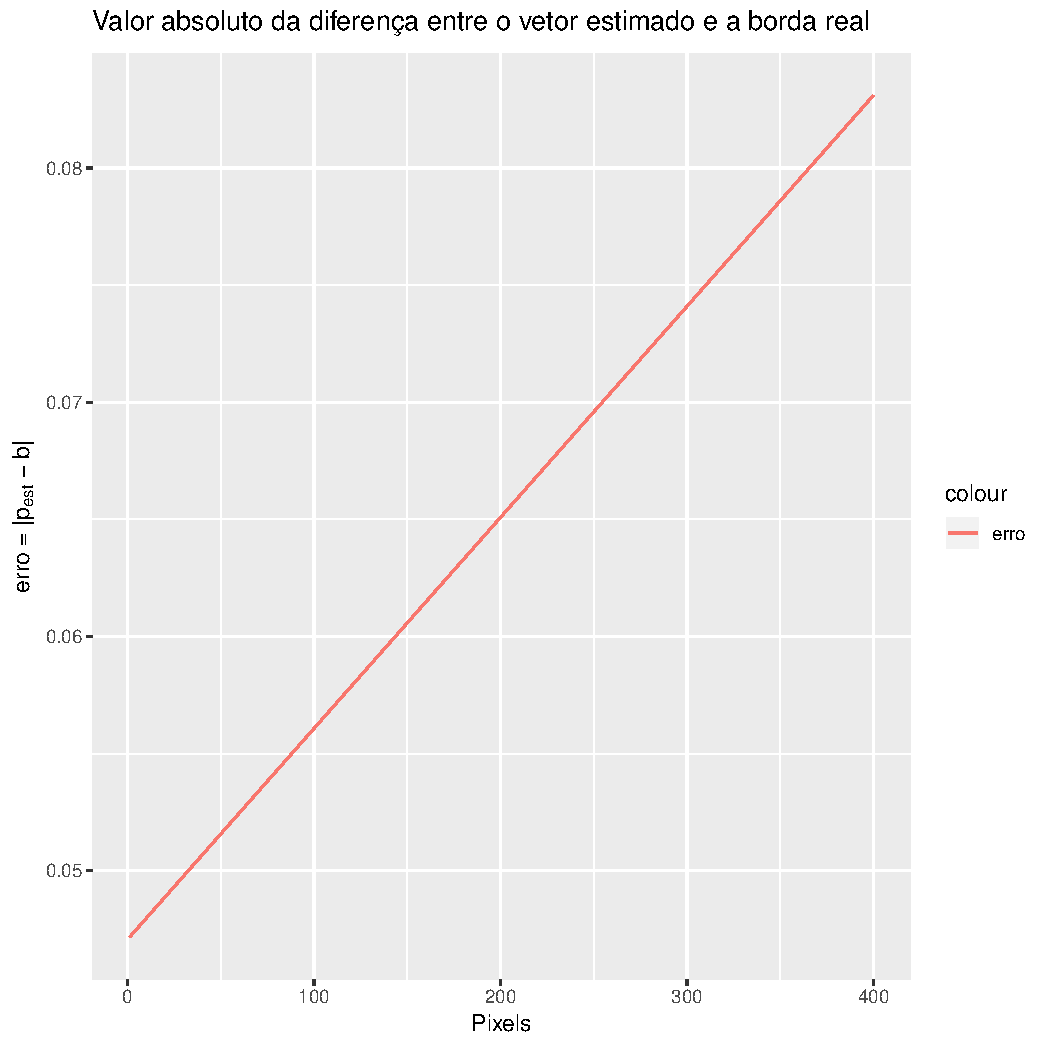
\includegraphics[width=\linewidth]{fusao_ls_erro_gamf.pdf}}	
%	\caption{Valor absoluto da diferença entre o vetor estimado da fusão de evidências e a borda real.}
%\label{cap_acf_fig14}
%\endminipage\hfill
%\end{figure}
%\section{Sigmas do artigo}
%\begin{figure}[hbt]
%\centering
%	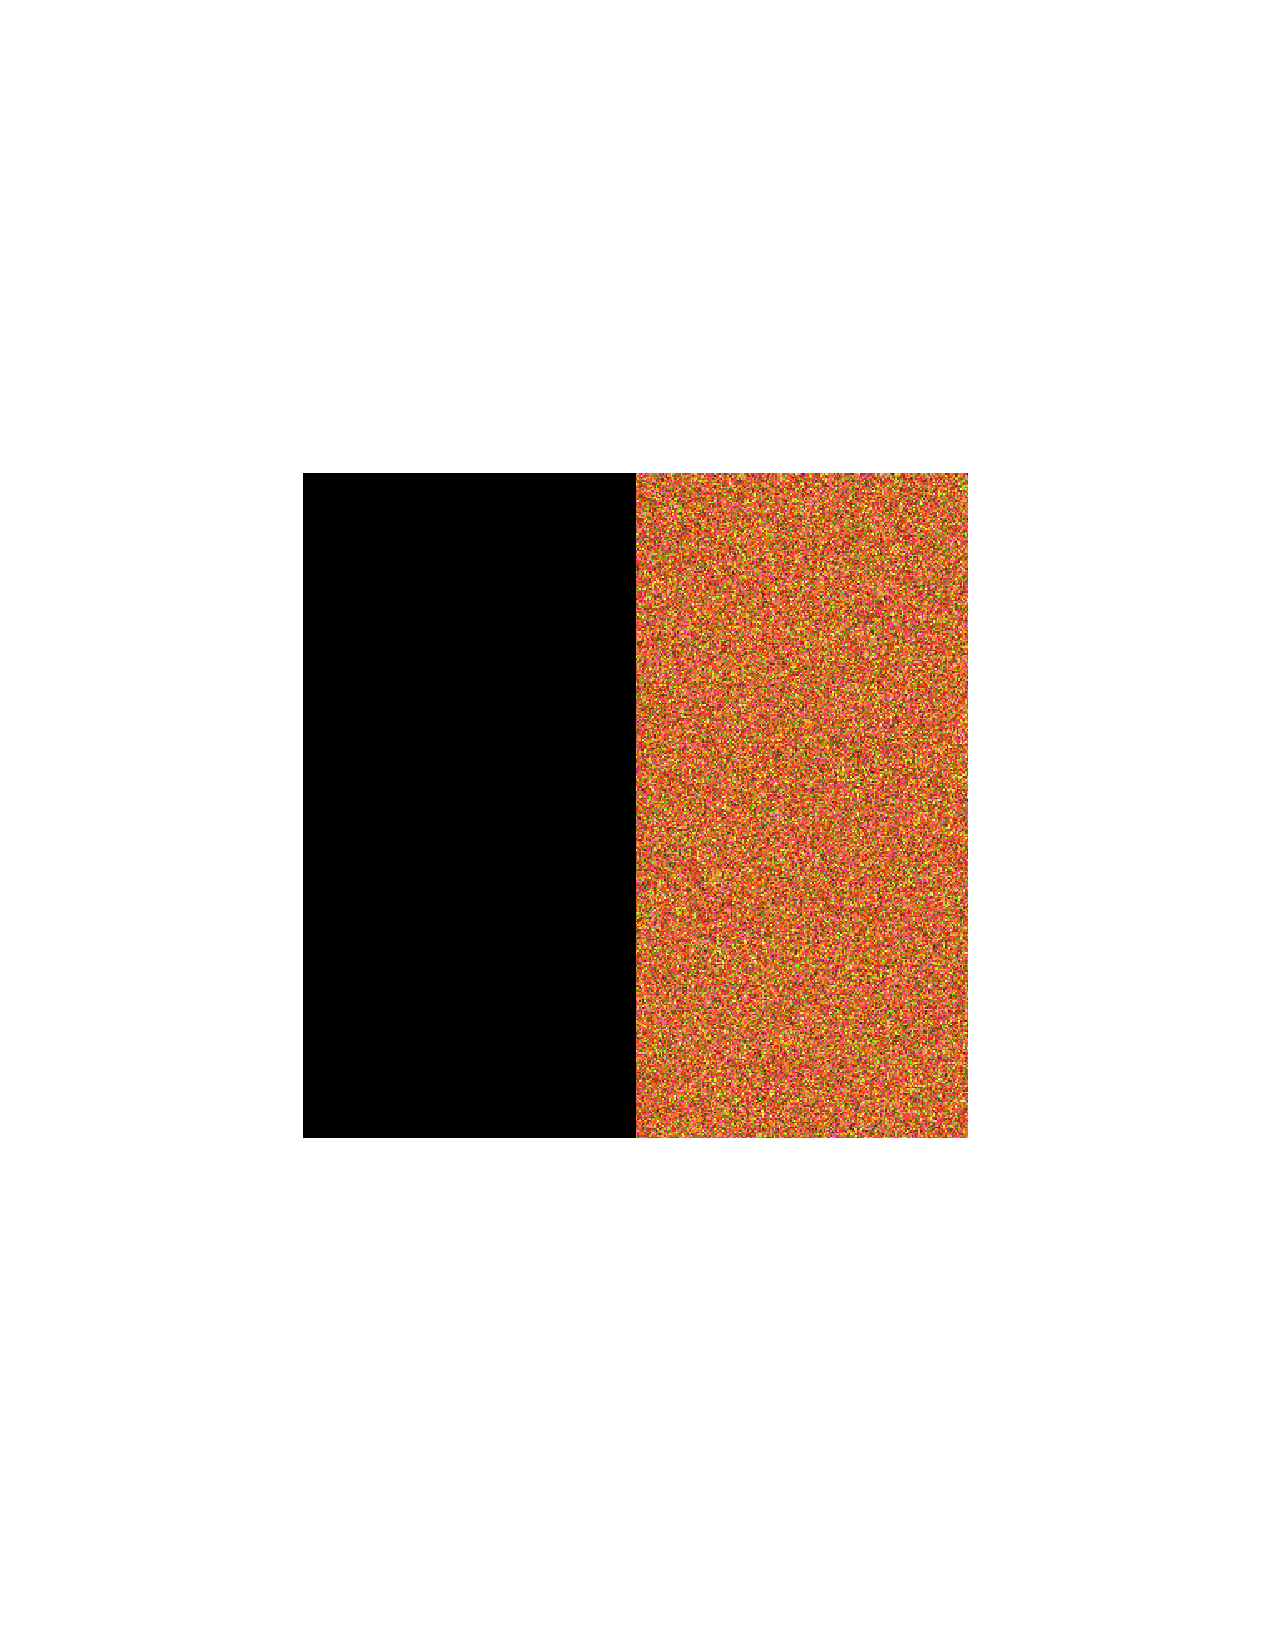
\includegraphics[width=5.0in]{phanton_vert_dec_pauli.pdf}
%	\caption{Decomposição de Pauli uma das phantons com valores de $\Sigma$ propostos no artigo \citep{gamf}.}\label{cap_acf_fig01}
%\end{figure}
%\begin{figure}[hbt]
%\minipage{0.5\textwidth}
%  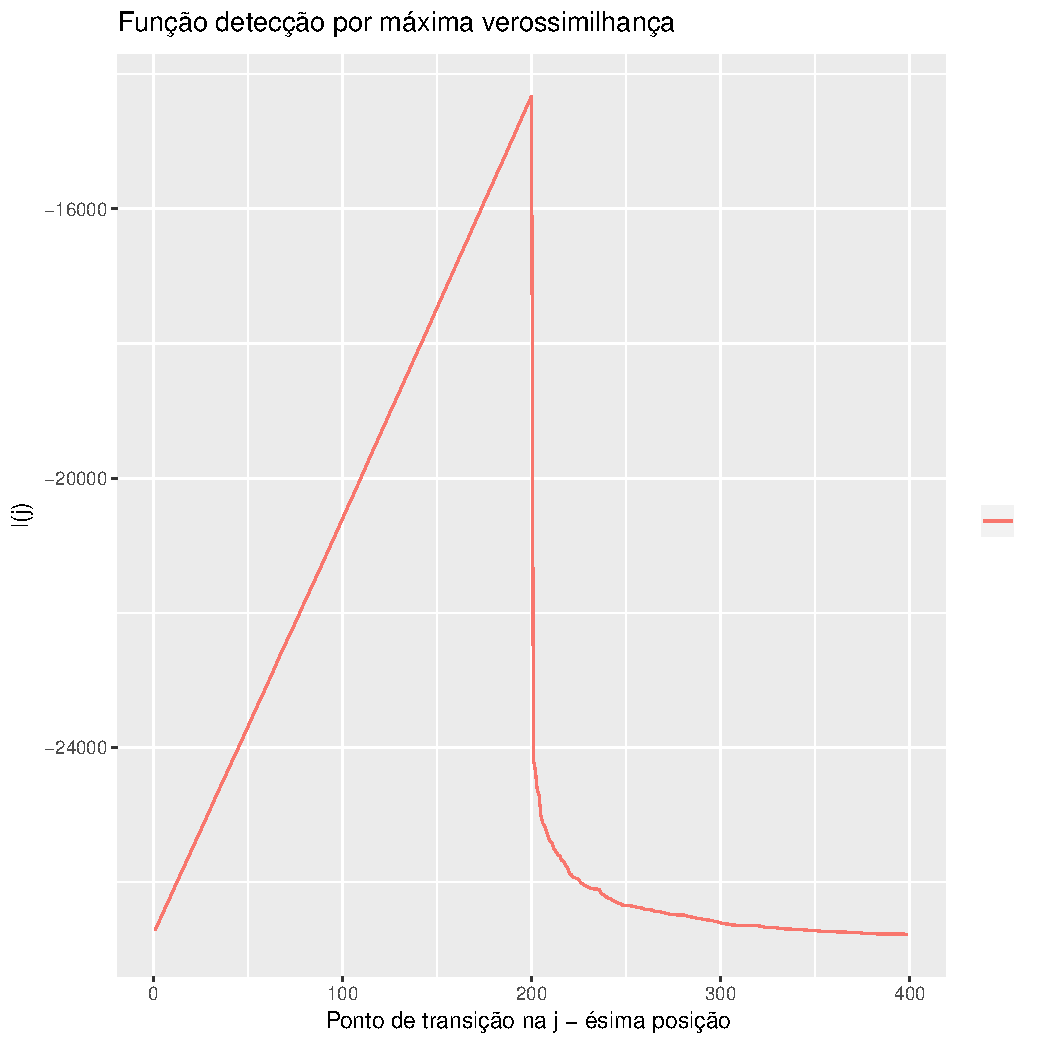
\includegraphics[width=\linewidth]{grafico_l_vert_sigmahh.pdf}
%	\caption{Função $l(j)$ para o canal $I_{HH}$}\label{cap_acf_fig04}
%\endminipage\hfill
%\minipage{0.5\textwidth}
%  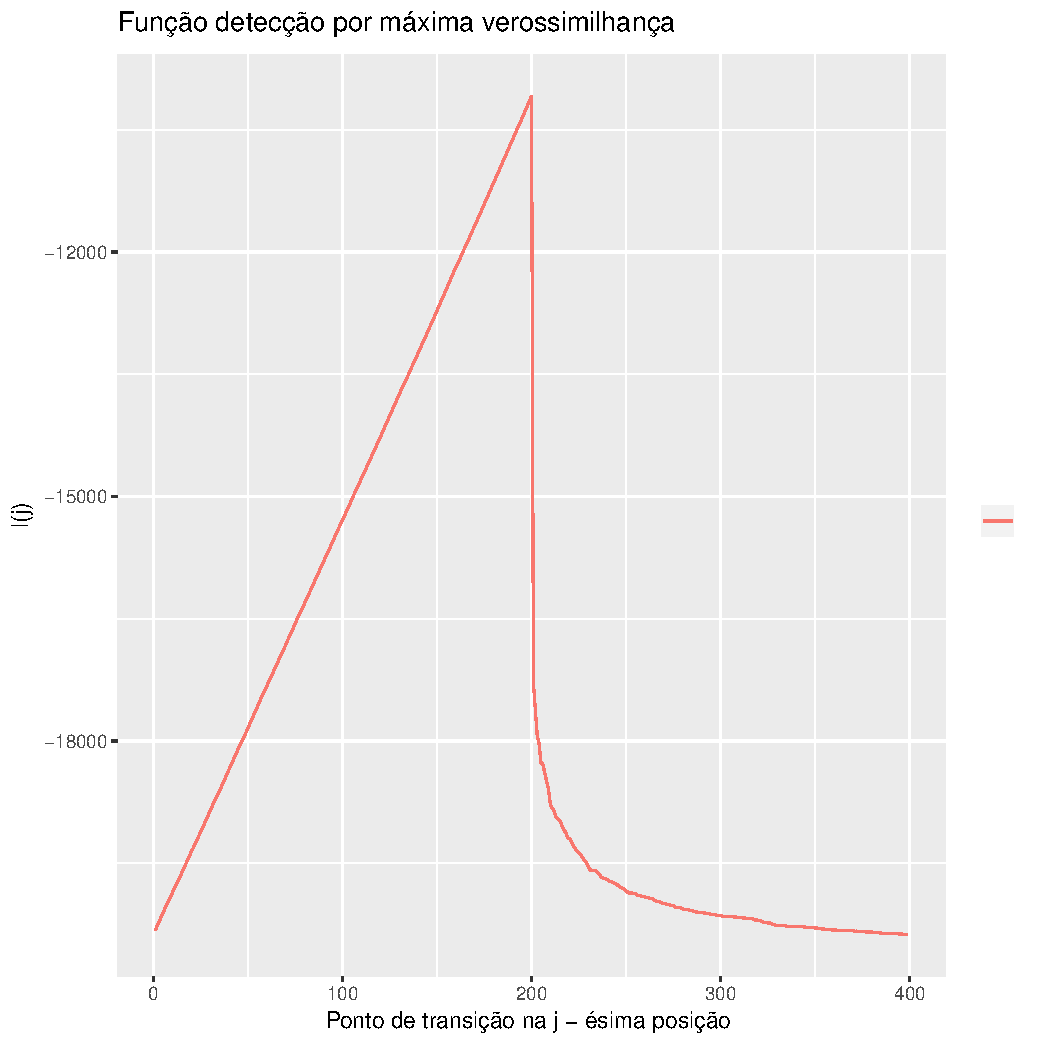
\includegraphics[width=\linewidth]{grafico_l_vert_sigmahv.pdf}
%	\caption{Função $l(j)$ para o canal $I_{HV}$}\label{cap_acf_fig05}
%\endminipage\hfill
%\centering
%\minipage{0.5\textwidth}
%  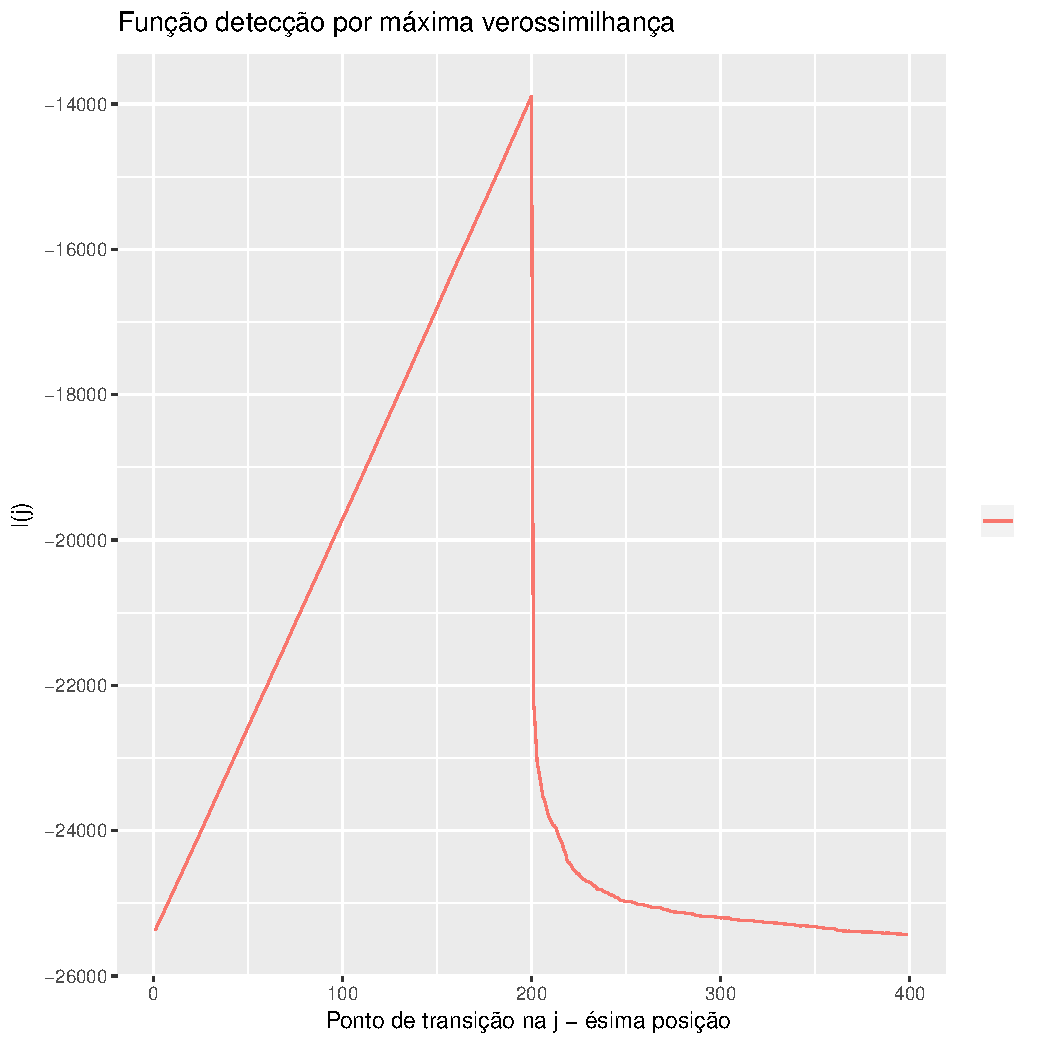
\includegraphics[width=\linewidth]{grafico_l_vert_sigmavv.pdf}
%	\caption{Função $l(j)$ para o canal $I_{VV}$}\label{cap_acf_fig06}
%\endminipage\hfill
%\end{figure}
%\begin{figure}[hbt]
%\minipage{0.475\textwidth}
%\fbox{  
\includegraphics[width=\linewidth]{ev_hh_vert.pdf}}
%\caption{Evidências de bordas para o canal $I_{HH}$}\label{cap_acf_fig07}
%\endminipage\hfill
%\minipage{0.475\textwidth}
%\fbox{ 
\includegraphics[width=\linewidth]{ev_hv_vert.pdf}}
%\caption{Evidências de bordas para o canal $I_{HV}$}\label{cap_acf_fig08}
%\endminipage\hfill
%\centering
%\minipage{0.475\textwidth}
%\fbox{ 
\includegraphics[width=\linewidth]{ev_vv_vert.pdf}}
%\caption{Evidências de bordas para o canal $I_{VV}$}\label{cap_acf_fig09}
%\endminipage\hfill
%\end{figure}
%\begin{figure}[hbt]
%\centering
%	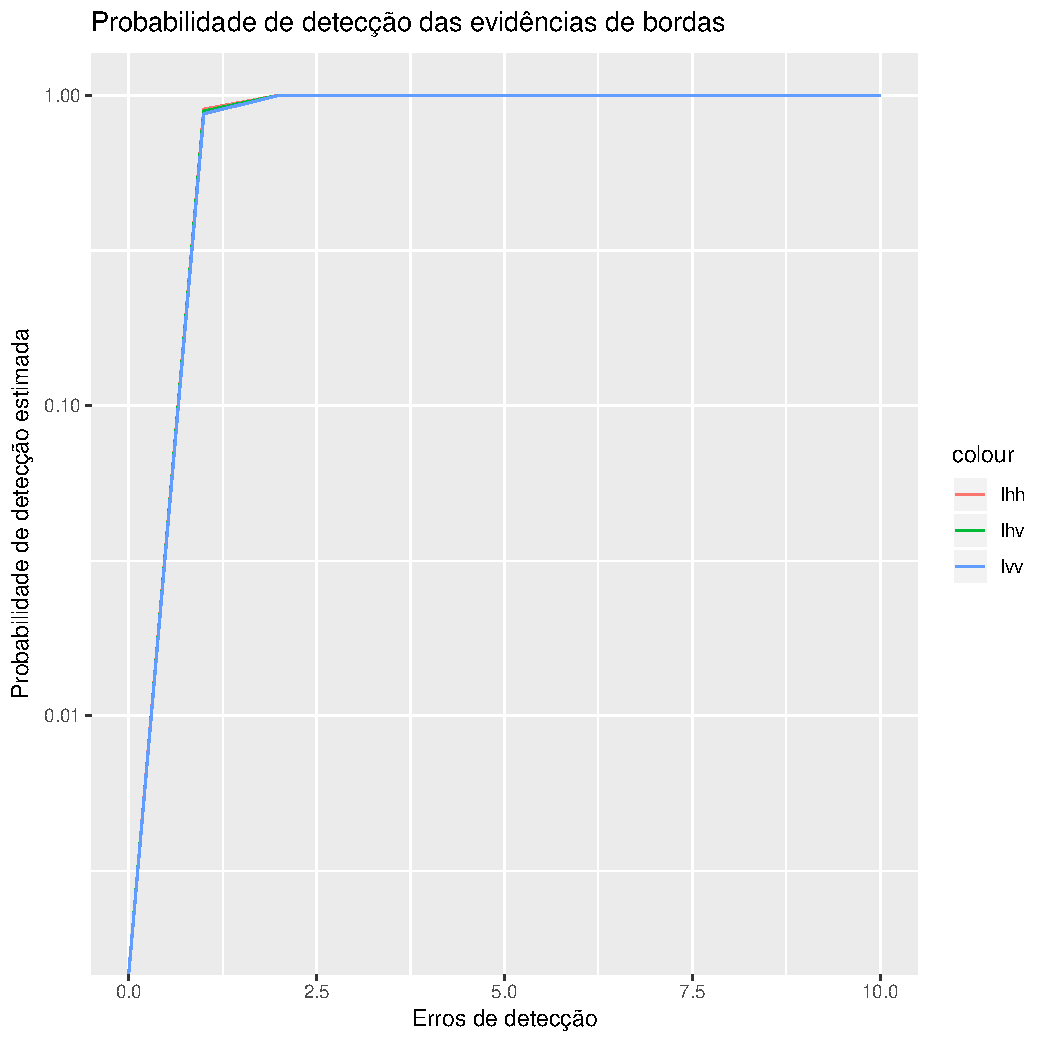
\includegraphics[width=5.0in]{metricas_ihh_ivh_ivv_vert.pdf}
%	\caption{Probabilidade de detecção de borda estimada usando GenSA.}
%\label{cap_acf_fig10}
%\end{figure}
%
%\begin{figure}[hbt]
%\minipage{0.475\textwidth}
%	\fbox{
\includegraphics[width=\linewidth]{fusao_soma_ev_hh_hv_vv_vert.pdf}}
%	\caption{Fusão de evidências para os canais $\left(I_{hh}, I_{hv}, I_{vv}\right)$.}
%\label{cap_acf_fig11}
%\endminipage\hfill
%\minipage{0.475\textwidth}
%\fbox{
\includegraphics[width=\linewidth]{fusao_ls_vert.pdf}}	
%\caption{Método dos quadrados mínimos aplicado a fusão de imagens.}
%\label{cap_acf_fig12}
%\endminipage\hfill
%\end{figure}
%\begin{figure}[hbt]
%\minipage{0.475\textwidth}
%	\fbox{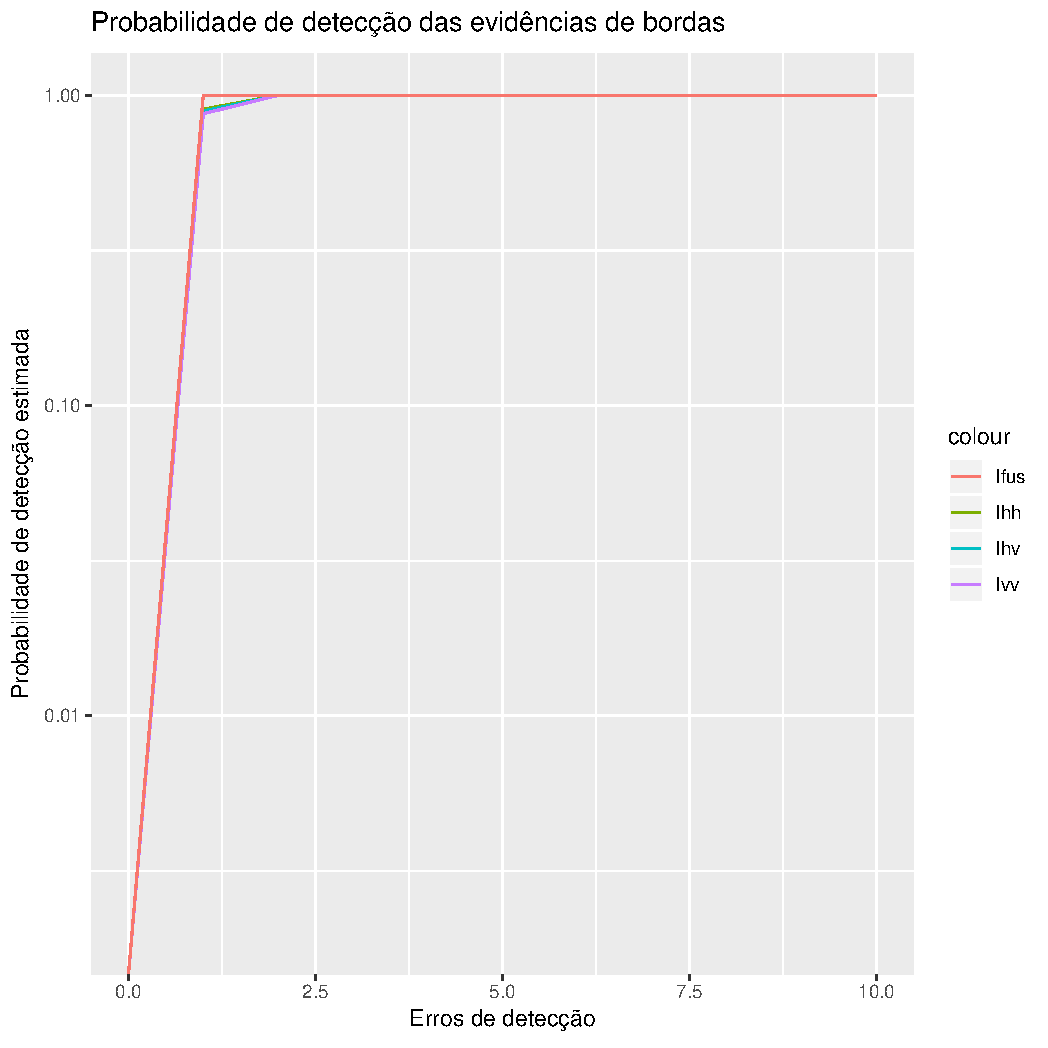
\includegraphics[width=\linewidth]{metricas_ihh_ivh_ivv_ils_vert.pdf}}
%	\caption{Probabilidade de detecção de borda com fusão de evidências.}
%\label{cap_acf_fig13}
%\endminipage\hfill
%\minipage{0.475\textwidth}
%\fbox{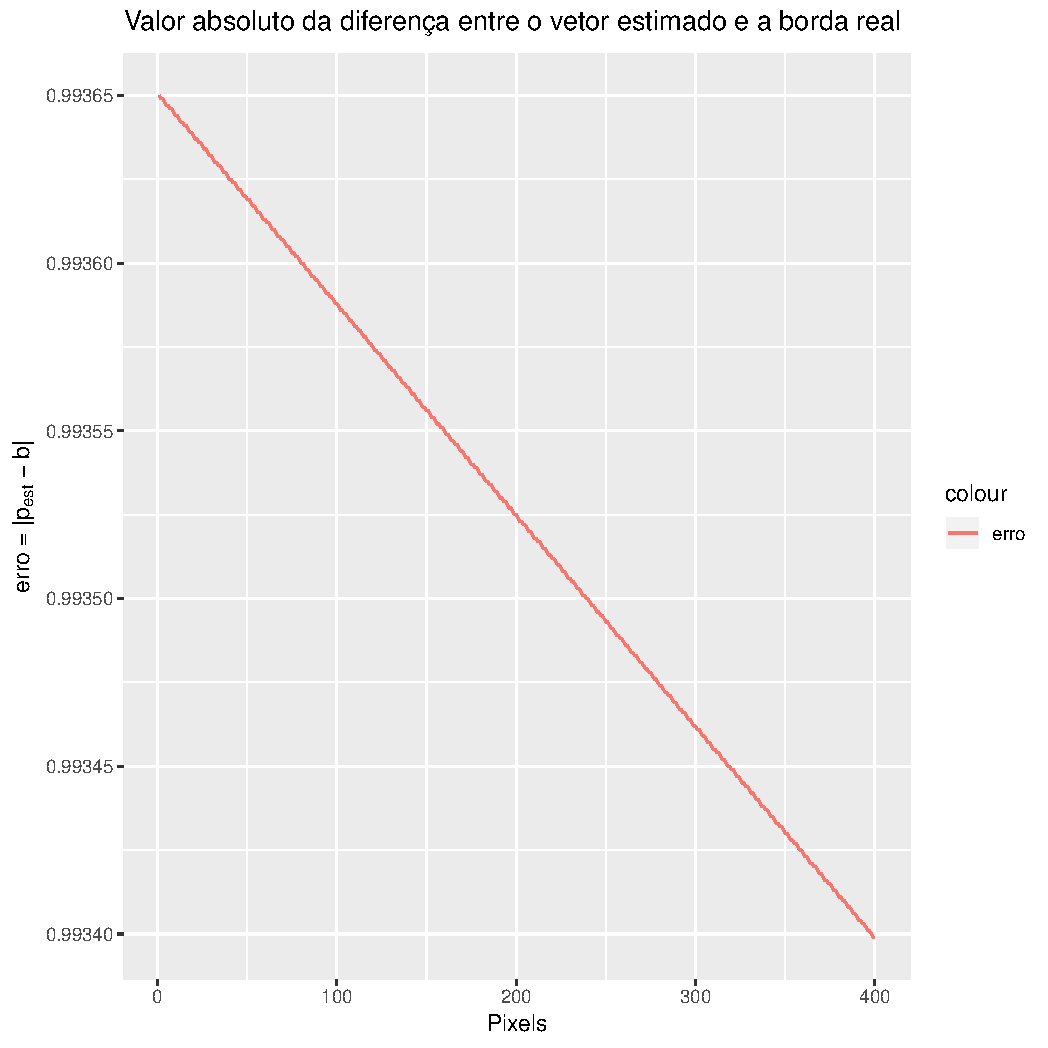
\includegraphics[width=\linewidth]{fusao_ls_erro_vert.pdf}}	
%	\caption{Valor absoluto da diferença entre o vetor estimado da fusão de evidências e a borda real.}
%\label{cap_acf_fig14}
%\endminipage\hfill
%\end{figure}

%%%%%%%%%%%%%%%%%%%%%%%%%%%%%
%%%%%%%%% Imagens de flores
%%%%%%%%%%%%%%%%%%%%%%%%%%
%Sigmas da referência \citet{nhfc}.
%\begin{figure}[hbt]
%\minipage{0.475\textwidth}
%	\fbox{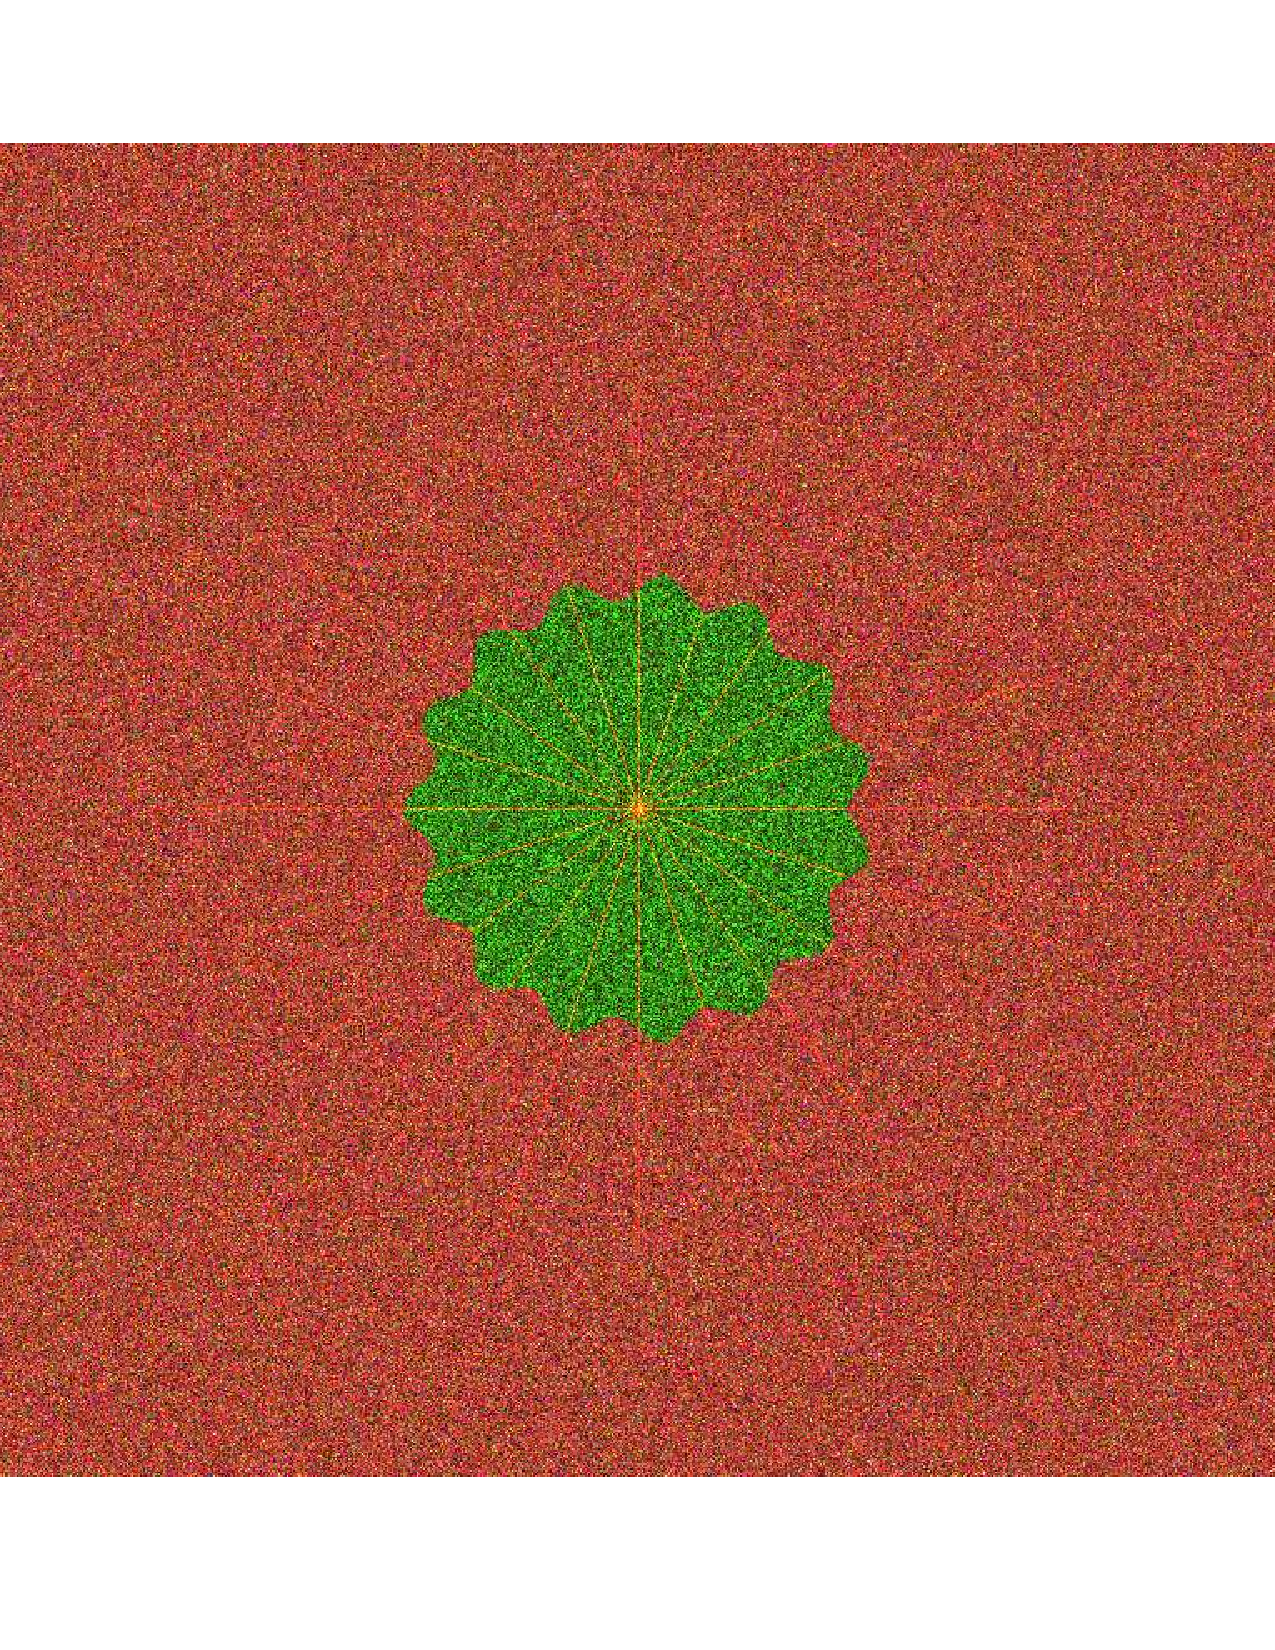
\includegraphics[width=\linewidth]{flor_15_133_8_pauli.pdf}}
%	\caption{Imagem flor simulada com $\beta = 15$, $\delta = 133$ e $\nu = 8$ .}
%\label{cap_acf_fig15}
%\endminipage\hfill
%\minipage{0.475\textwidth}
%\fbox{
\includegraphics[width=\linewidth]{flor_15_133_8_bin.pdf}}	
%	\caption{Imagem flor simulada binária com $\beta = 15$, $\delta = 133$ e $\nu = 8$ .}
%\label{cap_acf_fig16}
%\endminipage\hfill
%\end{figure}
%\begin{figure}[hbt]
%\minipage{0.475\textwidth}
%\fbox{  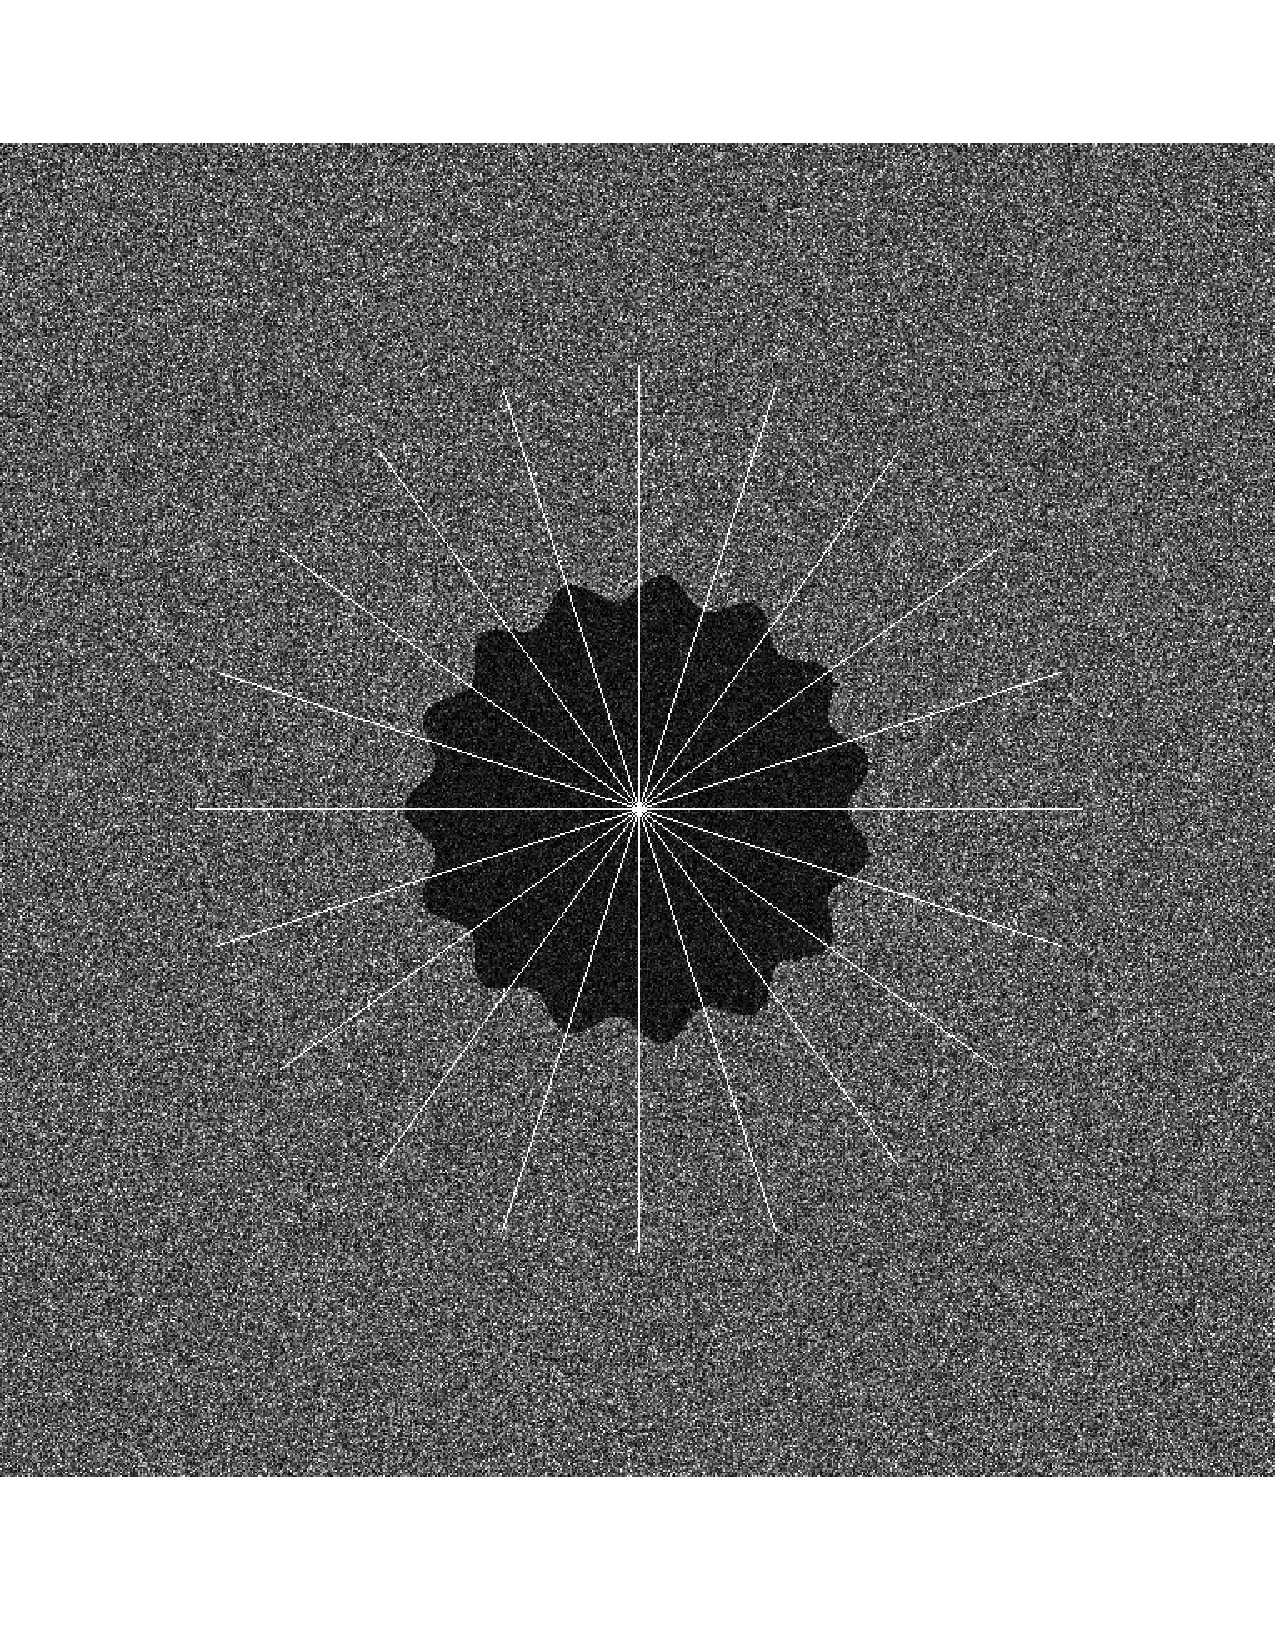
\includegraphics[width=\linewidth]{flor_15_133_8_hh.pdf}}
%	\caption{Imagem flor simulada canal $I_{hh}$ com $\beta = 15$, $\delta = 133$ e $\nu = 8$ .}
%\endminipage\hfill
%\minipage{0.475\textwidth}
%\fbox{ 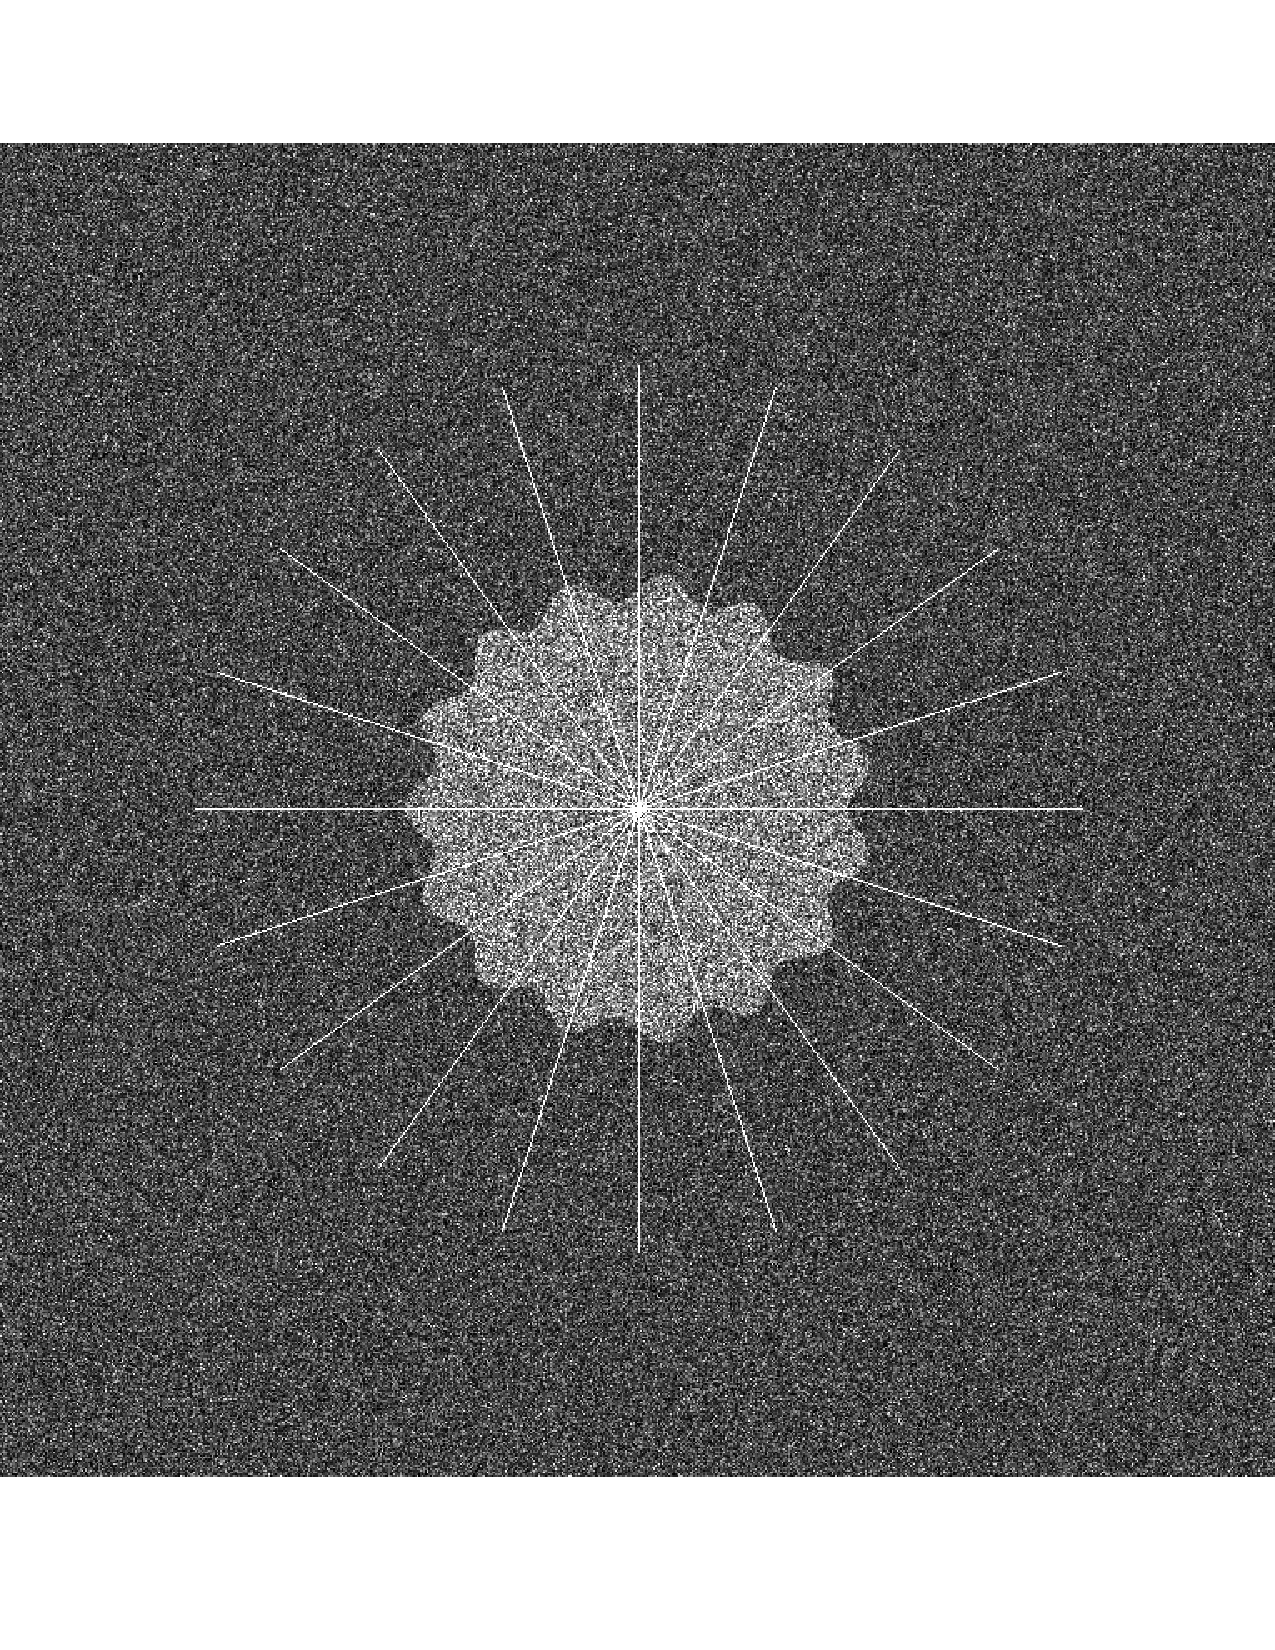
\includegraphics[width=\linewidth]{flor_15_133_8_hv.pdf}}
%	\caption{Imagem flor simulada canal $I_{hv}$ com $\beta = 15$, $\delta = 133$ e $\nu = 8$ .}
%\endminipage\hfill
%\centering
%\minipage{0.475\textwidth}
%\fbox{ 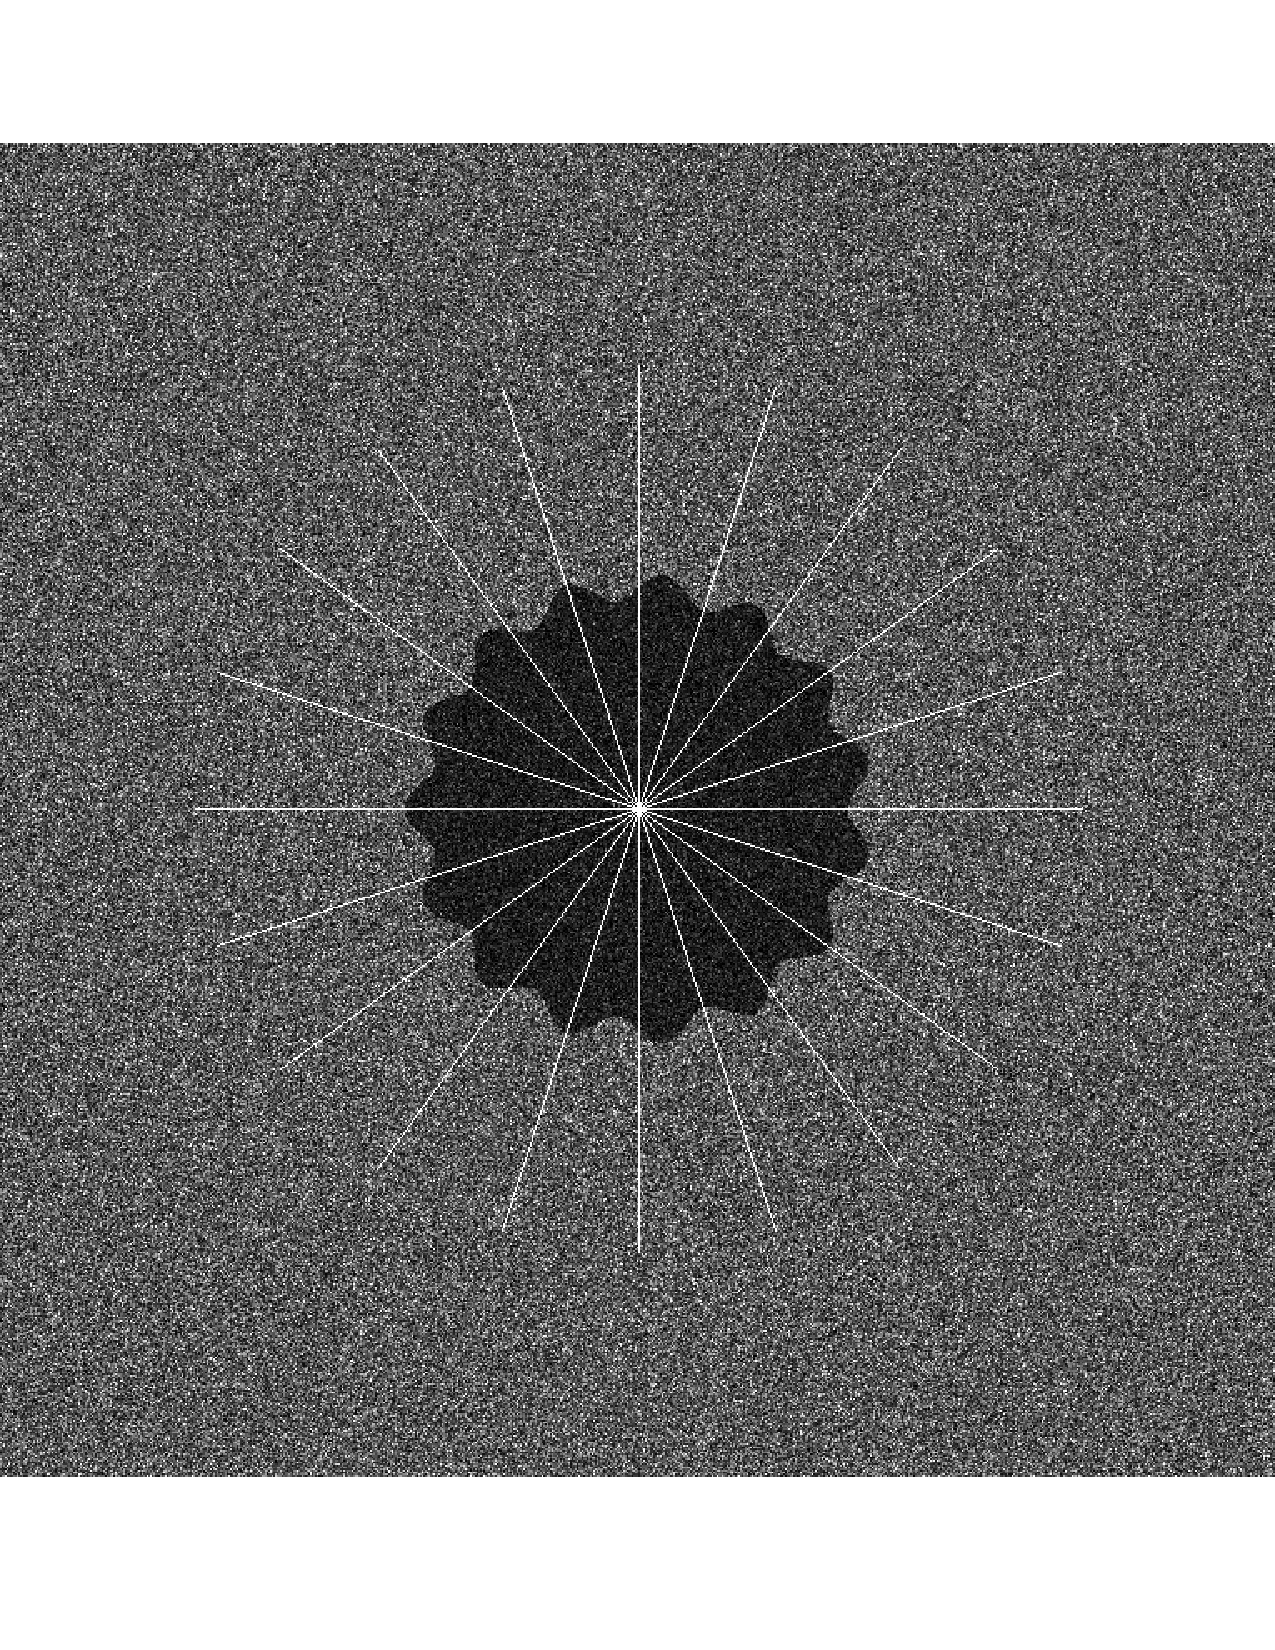
\includegraphics[width=\linewidth]{flor_15_133_8_vv.pdf}}
%	\caption{Imagem flor simulada canal $I_{vv}$ com $\beta = 15$, $\delta = 133$ e $\nu = 8$ .}
%\endminipage\hfill
%\end{figure}
%\begin{figure}[hbt]
%	\fbox{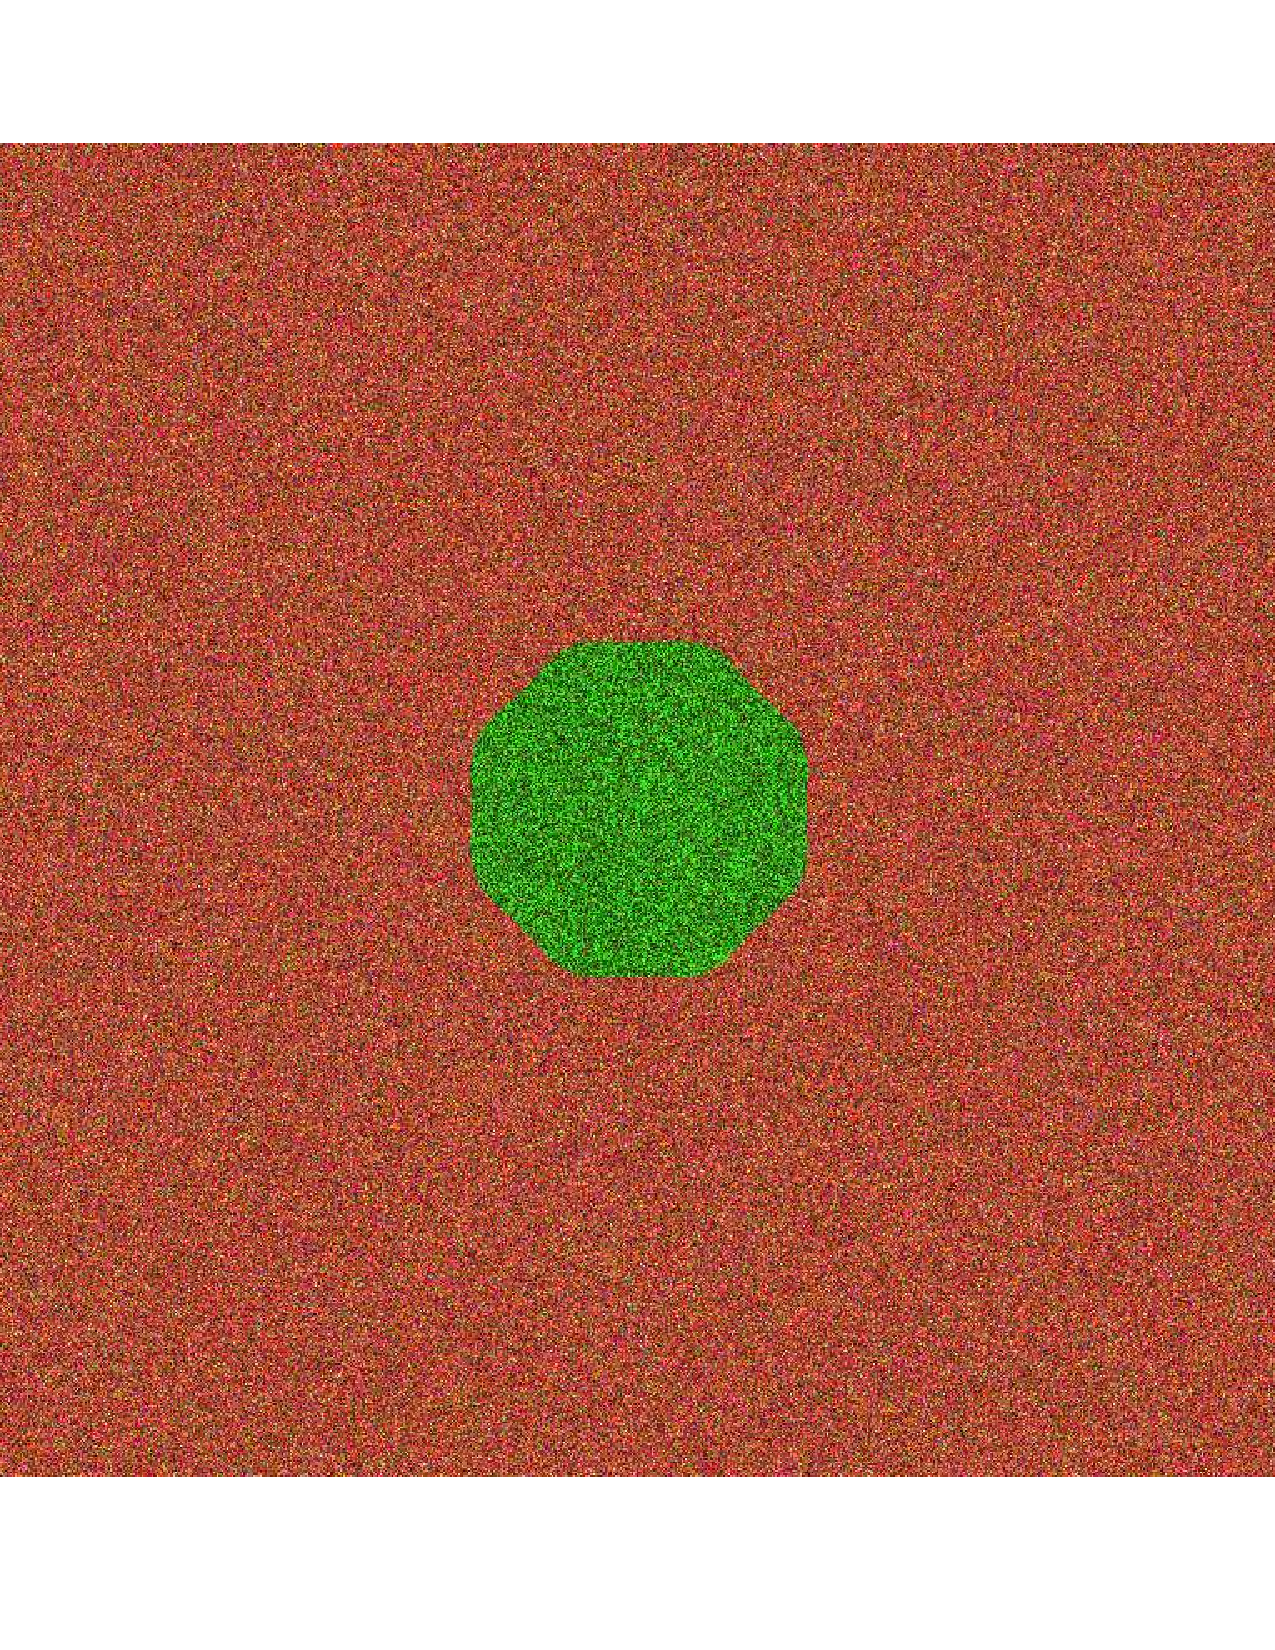
\includegraphics[width=\linewidth]{flor_8_103_3_pauli.pdf}}
%	\caption{Imagem flor simulada com $\beta = 8$, $\delta = 103$ e $\nu = 3$ .}
%\label{cap_acf_fig15}
%\end{figure}
%\begin{figure}[hbt]
%\minipage{0.475\textwidth}
%	\fbox{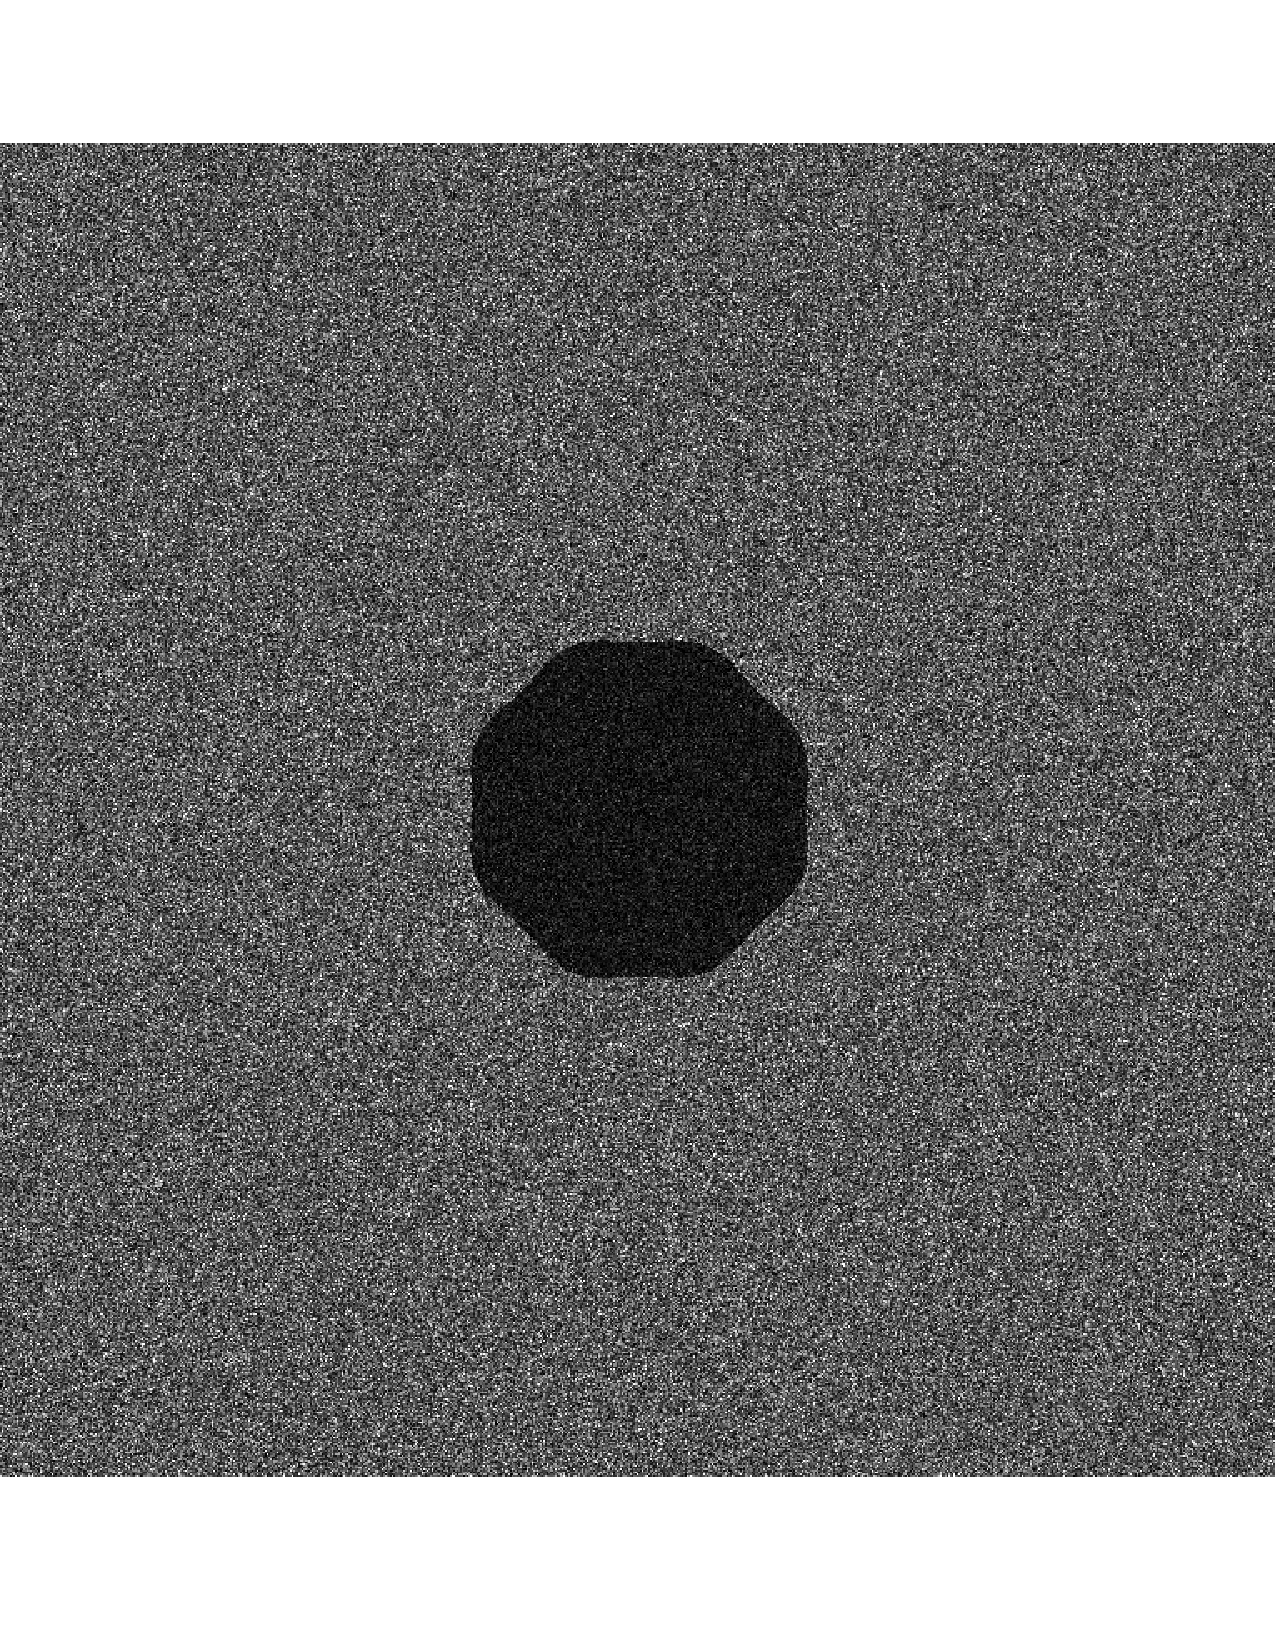
\includegraphics[width=\linewidth]{flor_8_103_3_hh.pdf}}
%	\caption{Imagem flor simulada canal $hh$ com $\beta = 8$, $\delta = 103$ e $\nu = 3$ .}
%\label{cap_acf_fig15}
%\endminipage\hfill
%\minipage{0.475\textwidth}
%	\fbox{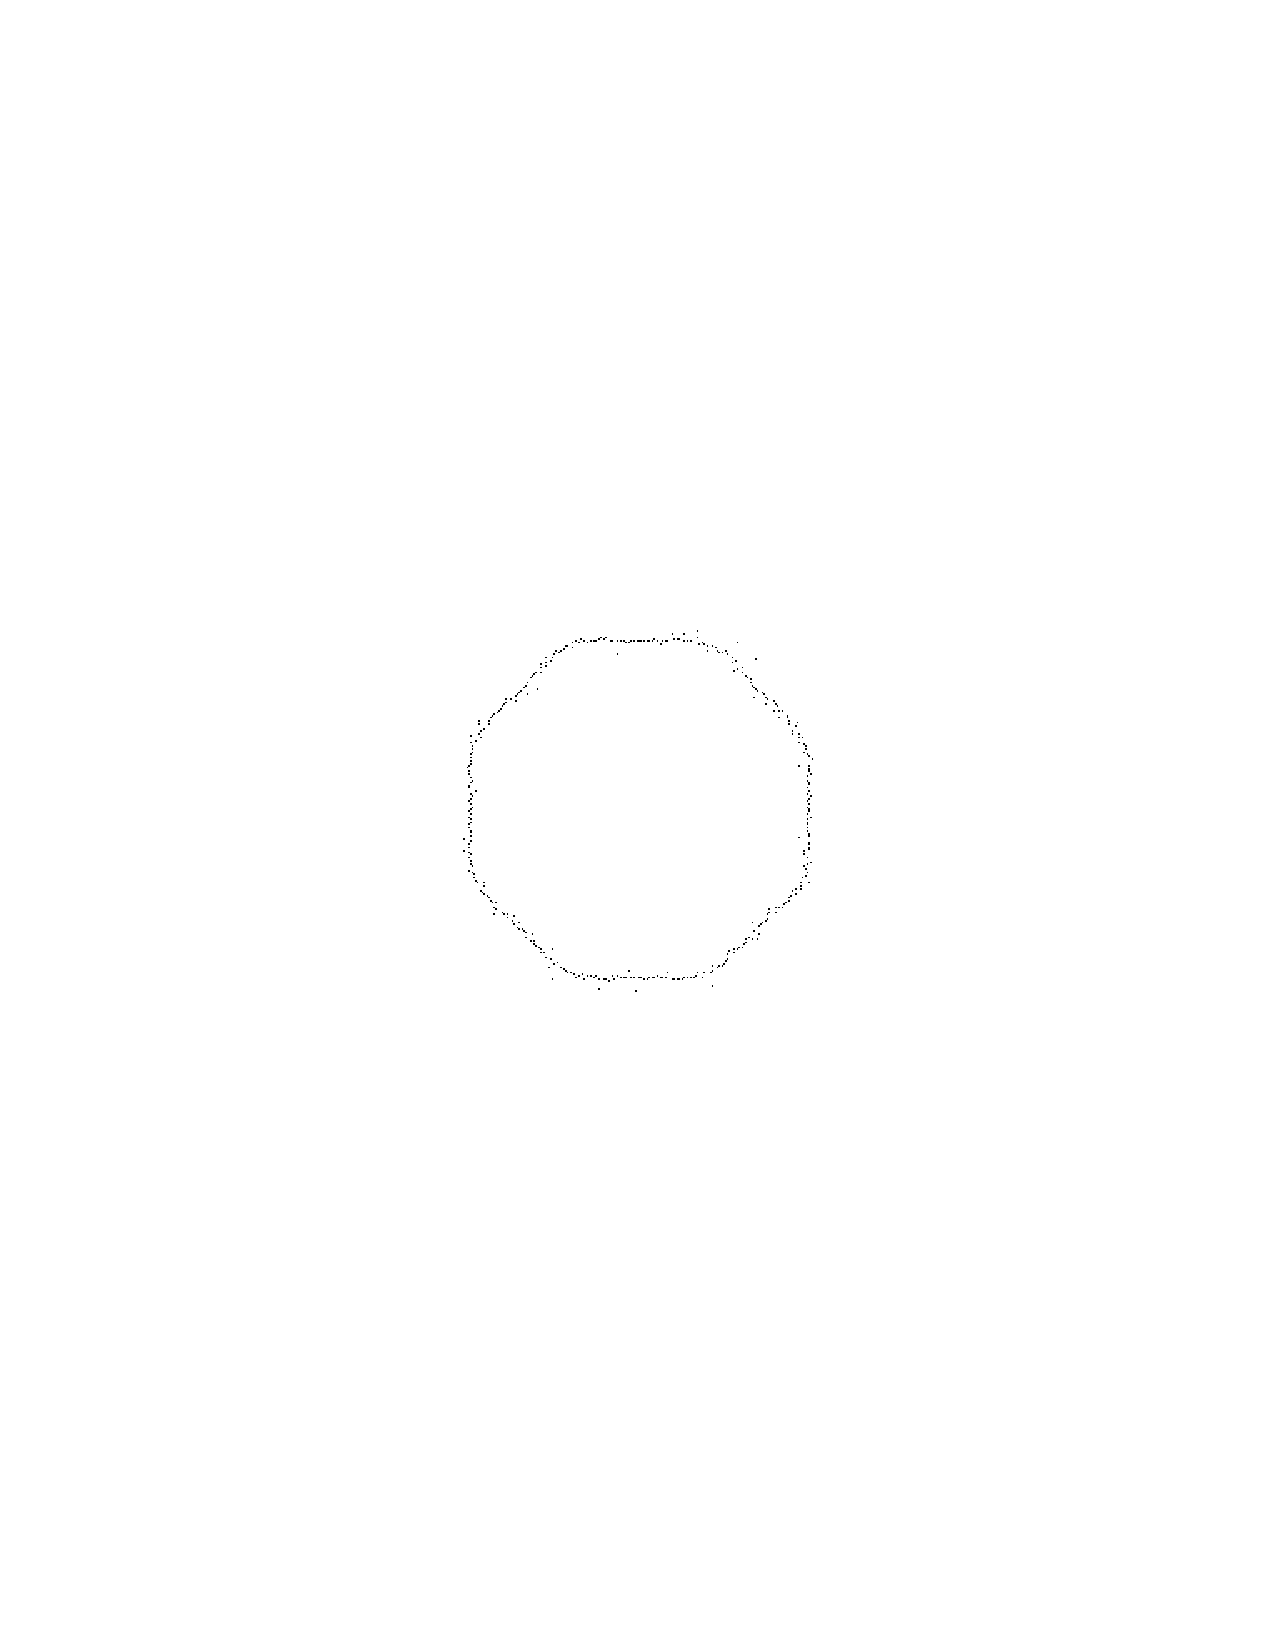
\includegraphics[width=\linewidth]{flor_evid_8_103_3_hh.pdf}}
%	\caption{Evidências de bordas canal $hh$ com $\beta = 8$, $\delta = 103$ e $\nu = 3$ .}
%\label{cap_acf_fig16}
%\endminipage\hfill
%\end{figure}
%\begin{figure}[hbt]
%\minipage{0.475\textwidth}
%	\fbox{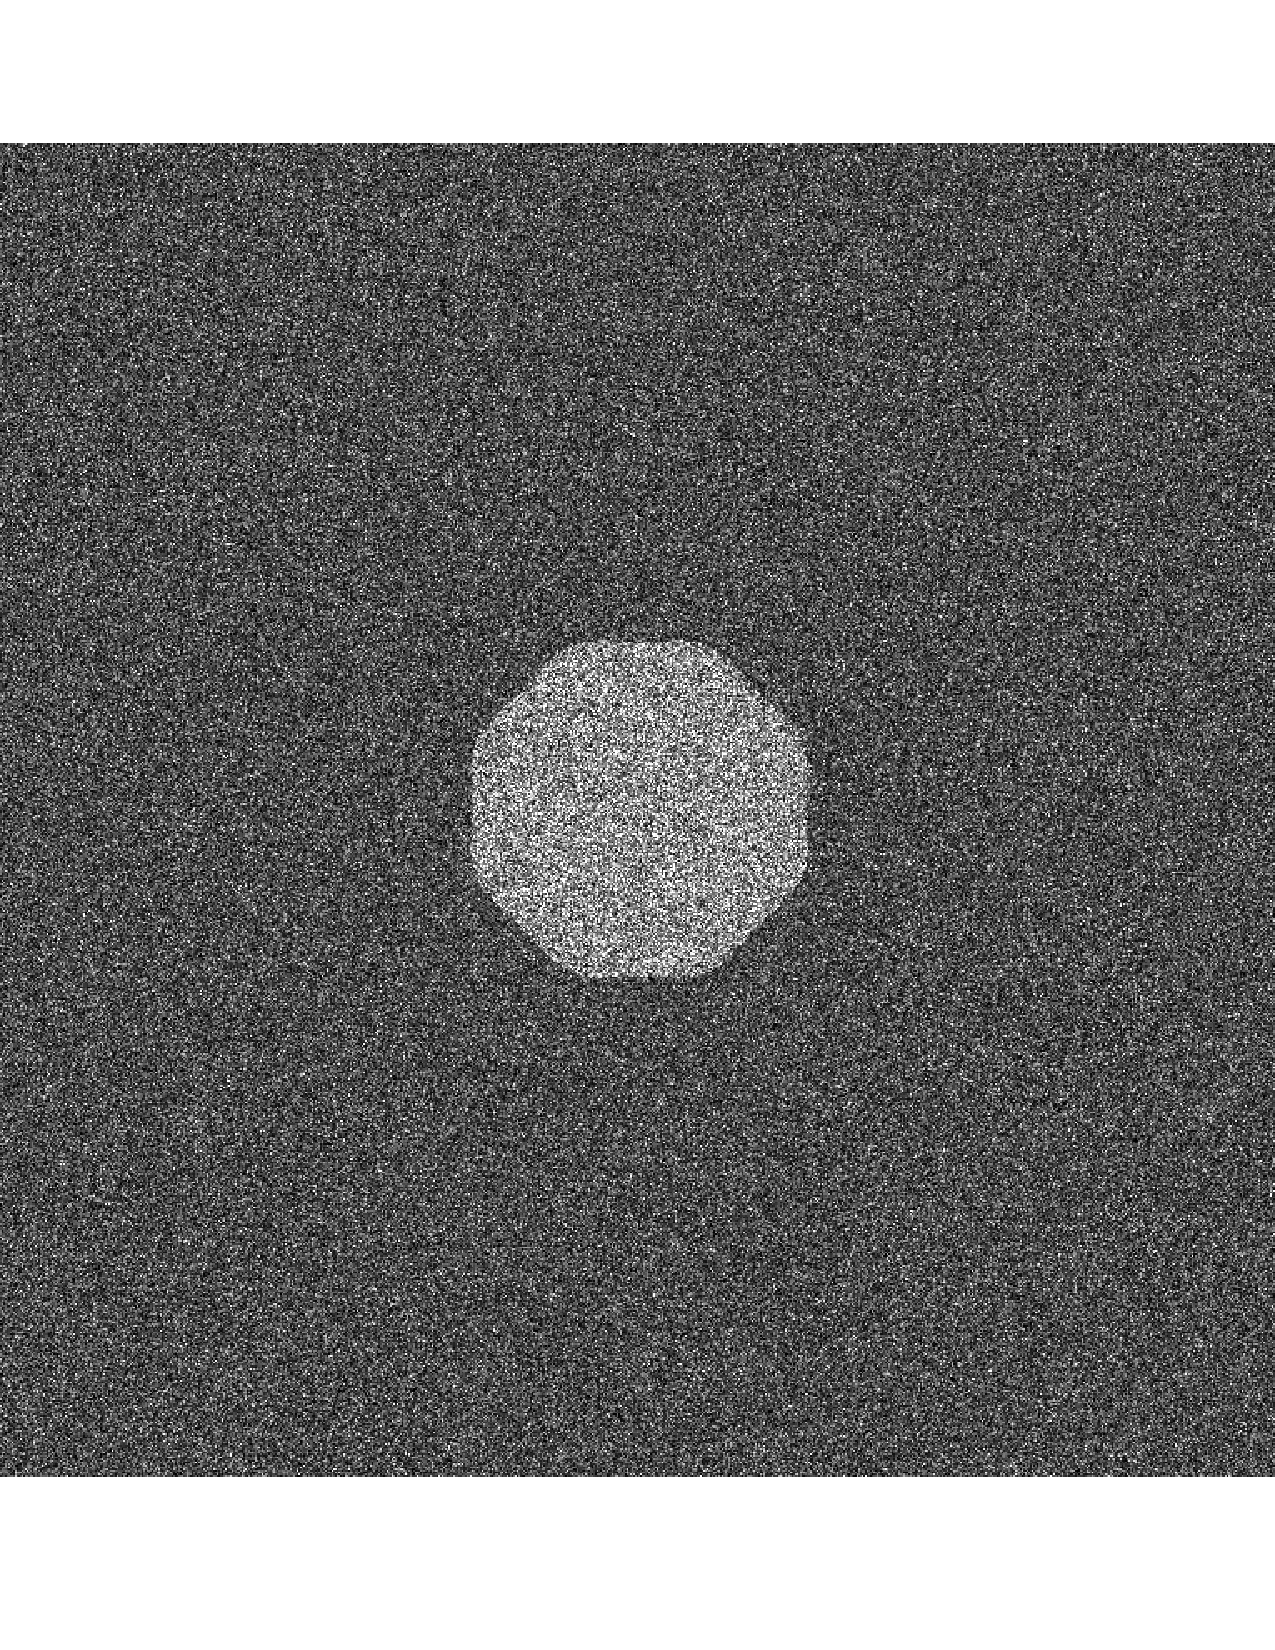
\includegraphics[width=\linewidth]{flor_8_103_3_hv.pdf}}
%	\caption{Imagem flor simulada canal $hv$ com $\beta = 8$, $\delta = 103$ e $\nu = 3$ .}
%\label{cap_acf_fig15}
%\endminipage\hfill
%\minipage{0.475\textwidth}
%	\fbox{\includegraphics[width=\linewidth]{flor_evid_8_103_3_hv.pdf}}
%	\caption{Evidências de bordas canal $hv$ com $\beta = 8$, $\delta = 103$ e $\nu = 3$ .}
%\label{cap_acf_fig16}
%\endminipage\hfill
%\end{figure}
%\begin{figure}[hbt]
%\minipage{0.475\textwidth}
%	\fbox{\includegraphics[width=\linewidth]{flor_8_103_3_vv.pdf}}
%	\caption{Imagem flor simulada canal $vv$ com $\beta = 8$, $\delta = 103$ e $\nu = 3$ .}
%\label{cap_acf_fig15}
%\endminipage\hfill
%\minipage{0.475\textwidth}
%	\fbox{\includegraphics[width=\linewidth]{flor_evid_8_103_3_vv.pdf}}
%	\caption{Evidencias de bordas canal $vv$ com $\beta = 8$, $\delta = 103$ e $\nu = 3$ .}
%\label{cap_acf_fig16}
%\endminipage\hfill
%\end{figure}
%\begin{figure}[hbt]
%	\fbox{\includegraphics[width=\linewidth]{flor_25_155_5_pauli.pdf}}
%	\caption{Imagem flor simulada com $\beta = 25$, $\delta = 155$ e $\nu = 5$ .}
%\label{cap_acf_fig15}
%\end{figure}
%\begin{figure}[hbt]
%\minipage{0.475\textwidth}
%	\fbox{\includegraphics[width=\linewidth]{flor_25_155_5_hh.pdf}}
%	\caption{Imagem flor simulada canal $hh$ com $\beta = 25$, $\delta = 155$ e $\nu = 5$ .}
%\label{cap_acf_fig15}
%\endminipage\hfill
%\minipage{0.475\textwidth}
%	\fbox{\includegraphics[width=\linewidth]{flor_evid_25_155_5_hh.pdf}}
%	\caption{Evidências de bordas canal $hh$ com $\beta = 25$, $\delta = 155$ e $\nu = 5$ .}
%\label{cap_acf_fig16}
%\endminipage\hfill
%\end{figure}
%\begin{figure}[hbt]
%\minipage{0.475\textwidth}
%	\fbox{\includegraphics[width=\linewidth]{flor_25_155_5_hv.pdf}}
%	\caption{Imagem flor simulada canal $hv$ com $\beta = 25$, $\delta = 155$ e $\nu = 5$ .}
%\label{cap_acf_fig15}
%\endminipage\hfill
%\minipage{0.475\textwidth}
%	\fbox{\includegraphics[width=\linewidth]{flor_evid_25_155_5_hv.pdf}}
%	\caption{Evidências de bordas canal $hv$ com $\beta = 25$, $\delta = 155$ e $\nu = 5$ .}
%\label{cap_acf_fig16}
%\endminipage\hfill
%\end{figure}
%\begin{figure}[hbt]
%\minipage{0.475\textwidth}
%	\fbox{\includegraphics[width=\linewidth]{flor_25_155_5_vv.pdf}}
%	\caption{Imagem flor simulada canal $vv$ com $\beta = 25$, $\delta = 155$ e $\nu = 5$ .}
%\label{cap_acf_fig15}
%\endminipage\hfill
%\minipage{0.475\textwidth}
%	\fbox{\includegraphics[width=\linewidth]{flor_evid_25_155_5_vv.pdf}}
%	\caption{Evidencias de bordas canal $vv$ com $\beta = 25$, $\delta = 155$ e $\nu = 5$ .}
%\label{cap_acf_fig16}
%\endminipage\hfill
%\end{figure}
\subsection{Distribuição gaussiana unidimensional para a intensidade com estimativa de parâmetros $L$ e $\mu$.}
\begin{figure}[hbt]
\minipage{0.5\textwidth}
  \includegraphics[width=\linewidth]{grafico_l_gamf_2017_sigmahh_param_L_mu.pdf}
	\caption{Função $l(j)$ para o canal $I_{HH}$}\label{cap_acf_fig04}
\endminipage\hfill
\minipage{0.5\textwidth}
  \includegraphics[width=\linewidth]{grafico_l_gamf_2017_sigmahv_param_L_mu.pdf}
	\caption{Função $l(j)$ para o canal $I_{HV}$}\label{cap_acf_fig05}
\endminipage\hfill
\centering
\minipage{0.5\textwidth}
  \includegraphics[width=\linewidth]{grafico_l_gamf_2017_sigmavv_param_L_mu.pdf}
	\caption{Função $l(j)$ para o canal $I_{VV}$}\label{cap_acf_fig06}
\endminipage\hfill
\end{figure}

\begin{figure}[hbt]
\minipage{0.5\textwidth}
  \includegraphics[width=\linewidth]{grafico_l_nhfc_2014_sigmahh_param_L_mu.pdf}
	\caption{Função $l(j)$ para o canal $I_{HH}$}\label{cap_acf_fig04}
\endminipage\hfill
\minipage{0.5\textwidth}
  \includegraphics[width=\linewidth]{grafico_l_nhfc_2014_sigmahv_param_L_mu.pdf}
	\caption{Função $l(j)$ para o canal $I_{HV}$}\label{cap_acf_fig05}
\endminipage\hfill
\centering
\minipage{0.5\textwidth}
  \includegraphics[width=\linewidth]{grafico_l_nhfc_2014_sigmavv_param_L_mu.pdf}
	\caption{Função $l(j)$ para o canal $I_{VV}$}\label{cap_acf_fig06}
\endminipage\hfill
\end{figure}


